        %%---------------------%%
        %%					   %%	
        %%	  TESI TRIENNALE   %%
        %%	   MAURO CARLIN    %%
        %%                     %%
        %%---------------------%%
\documentclass[10pt,                    % corpo del font principale
               a4paper,                 % carta A4
               twoside,                 % impagina per fronte-retro
               openright,               % inizio capitoli a destra
               english,                 
               italian,                 
               ]{book}    

\usepackage[utf8]{inputenc}             % codifica di input; anche [latin1] va bene
                                        % NOTA BENE! va accordata con le preferenze dell'editor

%**************************************************************
% Importazione package
%************************************************************** 

%\usepackage{amsmath,amssymb,amsthm}    % matematica

\usepackage[english, italian]{babel}    % per scrivere in italiano e in inglese;
                                        % l'ultima lingua (l'italiano) risulta predefinita

\usepackage{bookmark}                   % segnalibri

\usepackage{caption}                    % didascalie

\usepackage{chngpage,calc}              % centra il frontespizio

\usepackage{csquotes}                   % gestisce automaticamente i caratteri (")

\usepackage{emptypage}                  % pagine vuote senza testatina e piede di pagina

\usepackage{epigraph}					% per epigrafi

\usepackage{eurosym}                    % simbolo dell'euro

\usepackage[T1]{fontenc}                % codifica dei font:
                                        % NOTA BENE! richiede una distribuzione *completa* di LaTeX

%\usepackage{indentfirst}               % rientra il primo paragrafo di ogni sezione

\usepackage{graphicx}                   % immagini

\usepackage{hyperref}                   % collegamenti ipertestuali



\usepackage[binding=5mm]{layaureo}      % margini ottimizzati per l'A4; rilegatura di 5 mm

\usepackage{listings}                   % codici

\usepackage{microtype}                  % microtipografia

\usepackage{mparhack,fixltx2e,relsize}  % finezze tipografiche

\usepackage{nameref}                    % visualizza nome dei riferimenti                                      

\usepackage[font=small]{quoting}        % citazioni

\usepackage{subfigure}                  % sottofigure, sottotabelle

\usepackage[italian]{varioref}          % riferimenti completi della pagina

\usepackage[dvipsnames]{xcolor}         % colori

\usepackage{tabulary}
\usepackage{booktabs}                   % tabelle                                       
\usepackage{tabularx}                   % tabelle di larghezza prefissata                                    
\usepackage{longtable}                  % tabelle su più pagine                                        
\usepackage{ltxtable}                   % tabelle su più pagine e adattabili in larghezza
\newcolumntype{U}{>{\centering\arraybackslash}m{2cm}}
\newcolumntype{P}{>{\centering\arraybackslash}m{3cm}}
\newcolumntype{Z}{>{\centering\arraybackslash}m{4.2cm}}

\usepackage[toc, acronym]{glossaries}   % glossario
                                        % per includerlo nel documento bisogna:
                                        % 1. compilare una prima volta tesi.tex;
                                        % 2. eseguire: makeindex -s tesi.ist -t tesi.glg -o tesi.gls tesi.glo
                                        % 3. eseguire: makeindex -s tesi.ist -t tesi.alg -o tesi.acr tesi.acn
                                        % 4. compilare due volte tesi.tex.

\usepackage[backend=bibtex,style=verbose-ibid,hyperref,backref]{biblatex}
                                        % eccellente pacchetto per la bibliografia; 
                                        % produce uno stile di citazione autore-anno; 
                                        % lo stile "numeric-comp" produce riferimenti numerici
                                        % per includerlo nel documento bisogna:
                                        % 1. compilare una prima volta tesi.tex;
                                        % 2. eseguire: biber tesi
                                        % 3. compilare ancora tesi.tex.
                                        

%**************************************************************
% file contenente le impostazioni della tesi
%**************************************************************

%**************************************************************
% generale
%**************************************************************

% Azienda
\newcommand{\azienda}{i-contact s.r.l.}

%**************************************************************
% Frontespizio
%**************************************************************

% Autore
\newcommand{\myName}{Mauro Carlin}                                    
\newcommand{\myTitle}{Chatbot di Facebook Messenger per la risposta a domande frequenti}

% Tipo di tesi                   
\newcommand{\myDegree}{Tesi di laurea triennale}

% Università             
\newcommand{\myUni}{Università degli Studi di Padova}

% Facoltà       
\newcommand{\myFaculty}{Corso di Laurea in Informatica}

% Dipartimento
\newcommand{\myDepartment}{Dipartimento di Matematica "Tullio Levi-Civita"}

% Titolo del relatore
\newcommand{\profTitle}{Prof. }

% Relatore
\newcommand{\myProf}{Paolo Baldan}

% Luogo
\newcommand{\myLocation}{Padova}

% Anno accademico
\newcommand{\myAA}{2016-2017}

% Data discussione
\newcommand{\myTime}{Dicembre 2017}


%**************************************************************
% Impostazioni di impaginazione
% see: http://wwwcdf.pd.infn.it/AppuntiLinux/a2547.htm
%**************************************************************

\setlength{\parindent}{14pt}   % larghezza rientro della prima riga
\setlength{\parskip}{0pt}   % distanza tra i paragrafi


%**************************************************************
% Impostazioni di biblatex
%**************************************************************
\bibliography{bibliografia} % database di biblatex 

\defbibheading{bibliography} {
    \cleardoublepage
    \phantomsection 
    \addcontentsline{toc}{chapter}{\bibname}
    \chapter*{\bibname\markboth{\bibname}{\bibname}}
}

\setlength\bibitemsep{1.5\itemsep} % spazio tra entry

\DeclareBibliographyCategory{opere}
\DeclareBibliographyCategory{web}

\addtocategory{opere}{womak:lean-thinking}
\addtocategory{web}{site:agile-manifesto}

\defbibheading{opere}{\section*{Riferimenti bibliografici}}
\defbibheading{web}{\section*{Siti Web consultati}}


%**************************************************************
% Impostazioni di caption
%**************************************************************
\captionsetup{
    tableposition=top,
    figureposition=bottom,
    font=small,
    format=hang,
    labelfont=bf
}

%**************************************************************
% Impostazioni di glossaries
%**************************************************************

%**************************************************************
% Glossario
%**************************************************************
%\renewcommand{\glossaryname}{Glossario}

\newglossaryentry{ASD}
{
    name=\glslink{ASD}{Adaptive Software Development},
    text=Adaptive Software Development,
    description={\emph{L’Adaptive Software Development} (ASD) è una
metodologia composta da un insieme di regole di sviluppo software inserite in un
sistema complessivo detto \emph{Agile Project Management} i cui concetti base sono tre:
\begin{itemize}
	\item \emph{Leadership-Collaboration Management} - Uno stile di gestione misto fra gerarchico e collaborativo;
	\item \emph{emphFrom Processes to Pattern} - Passaggio dall’idea di processo definito e
misurabile a quella di processo non perfettamente definito, quasi un processo \emph{fuzzy};
	\item \emph{Peering into the Future} - Osservazione del futuro per capire come l’idea che produrrà un affare di successo debba essere legata al momento in cui diventerà una forma di business.
\end{itemize}}
}

\newglossaryentry{API}
{
    name=\glslink{API}{Application Program Interface},
    text=API,
    description={in informatica con il termine \emph{Application Programming
Interface} API (ing. interfaccia di programmazione di un’applicazione) si
indica ogni insieme di procedure disponibili al programmatore, di solito raggruppate
a formare un set di strumenti specifici per l’espletamento di un determinato
compito all’interno di un certo programma. La finalità è ottenere un’astrazione,
di solito tra l’hardware e il programmatore o tra software a basso e quello ad alto
livello semplificando così il lavoro di programmazione}
}

\newglossaryentry{AI}
{
    name=\glslink{AI}{Artificial Intelligence},
    text=AI,
    description={Definizioni specifiche possono essere date focalizzandosi o sui processi interni di ragionamento o sul comportamento esterno del sistema intelligente ed utilizzando come misura di efficacia o la somiglianza con il comportamento umano o con un comportamento ideale, detto razionale:
\begin{itemize}
	\item agire umanamente: il risultato dell’operazione compiuta dal sistema intelligente non è distinguibile da quella svolta da un umano.
	\item pensare umanamente: il processo che porta il sistema intelligente a risolvere un problema ricalca quello umano. Questo approccio è associato alle scienze cognitive.
	\item pensare razionalmente: il processo che porta il sistema intelligente a risolvere un problema è un procedimento formale che si rifà alla logica.
	\item agire razionalmente: il processo che porta il sistema intelligente a risolvere il problema è quello che gli permette di ottenere il miglior risultato atteso date le informazioni a disposizione
\end{itemize}}
}

\newglossaryentry{brainstorming}
{
    name=\glslink{brainstorming}{Brainstorming},
    text=brainstorming,
    description={L'espressione brainstorming, o brain storming (traducibile in lingua italiana come assalto mentale), è una tecnica creativa di gruppo per far emergere idee volte alla risoluzione di un problema}
}

\newglossaryentry{chatbot}
{
    name=\glslink{chatbot}{Chatbot},
    text=chatbot,
    description={in informatica con il termine \emph{Chatbot} si indica un programma che simula una conversazione tra un robot e un essere umano. Questi programmi funzionano o come utenti stessi delle \emph{chat} o come persone che rispondono alle FAQ delle persone che accedono al sito}
}

\newglossaryentry{CMS}
{
    name=\glslink{CMS}{Content management system},
    text=CMS,
    description={in informatica un \emph{content management system}, in acronimo CMS (sistema di gestione dei contenuti in italiano), è uno strumento software, installato su un server web, il cui compito è facilitare la gestione dei contenuti di siti web, svincolando il \emph{webmaster} da conoscenze tecniche specifiche di programmazione Web}
}

\newglossaryentry{diagramma di gantt}
{
    name=\glslink{diagramma di gantt}{Diagramma di Gantt},
    text=diagramma di Gantt,
    description={il diagramma di Gantt è uno strumento di supporto alla
gestione dei progetti, così chiamato in ricordo dell'ingegnere statunitense Henry
Laurence Gantt (1861-1919), che si occupava di scienze sociali e che lo ideò
nel 1917. Tale diagramma è usato principalmente nelle attività di \emph{project
management}, ed è costruito partendo da un asse orizzontale - a rappresentazione
dell’arco temporale totale del progetto, suddiviso in fasi incrementali (ad esempio,
giorni, settimane, mesi) - e da un asse verticale - a rappresentazione delle mansioni
o attività che costituiscono il progetto}
}

\newglossaryentry{XML}
{
    name=\glslink{XML}{Extensible Markup Language},
    text=XML,
    description={In informatica XML (sigla di \emph{eXtensible Markup Language}) è un metalinguaggio per la definizione di linguaggi di \emph{markup}, ovvero un linguaggio marcatore basato su un meccanismo sintattico che consente di definire e controllare il significato degli elementi contenuti in un documento o in un testo}
}

\newglossaryentry{FTP}
{
    name=\glslink{FTP}{File Transfer Protocol},
    text=FTP,
    description={in informatica il \emph{File Transfer Protocol} è un protocollo per la trasmissione di dati tra \emph{host} basato su \emph{TCP} e con architettura di tipo client-server. Il protocollo usa connessioni \emph{TCP} distinte per trasferire i dati e per controllare i trasferimenti e richiede autenticazione del client tramite nome utente e password}
}

\newglossaryentry{framework}
{
    name=\glslink{framework}{Framework},
    text=framework,
    description={un \emph{framework}, termine della lingua inglese che può essere tradotto come intelaiatura o struttura, in informatica e specificatamente nello sviluppo software, è un'architettura logica di supporto (spesso un'implementazione logica di un particolare \emph{design pattern}) su cui un software può essere progettato e realizzato, spesso facilitandone lo sviluppo da parte del programmatore},
    plural=frameworks
}

\newglossaryentry{FAQ}
{
    name=\glslink{FAQ}{Frequently Asked Questions},
    text=FAQ,
    description={Le \emph{Frequently Asked Questions}, meglio conosciute con la sigla FAQ, sono letteralmente le "domande poste frequentemente"; più esattamente sono una serie di risposte stilate direttamente dall'autore, in risposta alle domande che gli vengono poste, o che ritiene gli verrebbero poste, più frequentemente dagli utilizzatori di un certo servizio: soprattutto su Internet e in particolare nel web e nelle comunità virtuali vi sono domande ricorrenti alle quali si preferisce rispondere pubblicamente con un documento affinché non vengano poste troppo spesso, in modo da sciogliere i dubbi dei nuovi utenti}
}

\newglossaryentry{frontend}
{
    name=\glslink{frontend}{Frontend},
    text=frontend,
    description={termine che denota l’insieme delle applicazioni, relative ad una piattaforma
web, con le quali l’utente interagisce direttamente essendo la parte visibile da chiunque e raggiungibile all'indirizzo web del sito.}
}

\newglossaryentry{IDE}
{
    name=\glslink{IDE}{Integrated Development Environment},
    text=IDE,
    description={in informatica un ambiente di sviluppo
integrato (in lingua inglese \emph{integrated development environment} ovvero IDE,
anche integrated design environment o integrated debugging environment, rispettivamente
ambiente integrato di progettazione e ambiente integrato di \emph{debugging})
è un software che, in fase di programmazione, aiuta i programmatori nello sviluppo
del codice sorgente di un programma. Spesso l’IDE aiuta lo sviluppatore
segnalando errori di sintassi del codice direttamente in fase di scrittura, oltre a
tutta una serie di strumenti e funzionalità di supporto alla fase di sviluppo e
\emph{debugging}}
}

\newglossaryentry{JSON}
{
    name=\glslink{JSON}{JavaScript Object Notation},
    text=JSON,
    description={in informatica, nell’ambito della programmazione
web, JSON, acronimo di \emph{JavaScript Object Notation}, è un formato adatto
all’interscambio di dati fra applicazioni \emph{client-server}}
}

\newglossaryentry{NLP}
{
    name=\glslink{NLP}{Natural Language Processing},
    text=NLP,
    sort=nlp,
    description={in informatica con il termine \emph{Application Programming Interface API} (ing. interfaccia di programmazione di un'applicazione) si indica ogni insieme di procedure disponibili al programmatore, di solito raggruppate a formare un set di strumenti specifici per l'espletamento di un determinato compito all'interno di un certo programma. La finalità è ottenere un'astrazione, di solito tra l'hardware e il programmatore o tra software a basso e quello ad alto livello semplificando così il lavoro di programmazione}
}

\newglossaryentry{ORM}
{
    name=\glslink{ORM}{Object-relational mapping},
    text=ORM,
    description={In informatica l'\emph{Object-Relational Mapping} (ORM) è una tecnica di programmazione che favorisce l'integrazione di sistemi software aderenti al paradigma della programmazione orientata agli oggetti con sistemi RDBMS.
Un prodotto ORM fornisce, mediante un'interfaccia orientata agli oggetti, tutti i servizi inerenti alla persistenza dei dati, astraendo nel contempo le caratteristiche implementative dello specifico RDBMS utilizzato}
}

\newglossaryentry{open source}
{
    name=\glslink{open source}{Open source},
    text=open source,
    description={In informatica, il termine inglese \emph{open source} (che significa sorgente aperta) indica un software di cui gli autori (più precisamente, i detentori dei diritti) rendono pubblico il codice sorgente, favorendone il libero studio e permettendo a programmatori indipendenti di apportarvi modifiche ed estensioni. Questa possibilità è regolata tramite l'applicazione di apposite licenze d'uso. Il fenomeno ha tratto grande beneficio da Internet, perché esso permette a programmatori distanti di coordinarsi e lavorare allo stesso progetto}
}

\newglossaryentry{push}
{
    name=\glslink{push}{Notifica push},
    text=push,
    description={La notifica push è una tipologia di messaggistica istantanea con la quale il messaggio perviene al destinatario senza che questo debba effettuare un'operazione di scaricamento (modalità \emph{pull}). Tale modalità è quella tipicamente utilizzata da applicazioni come \emph{WhatsApp}, oppure servizi di sistemi operativi come \emph{Android}, o come numerose applicazioni derivate da siti web (ad esempio il classico servizio meteo o quello delle notizie).
Per permettere alle notifiche push di giungere al destinatario è indispensabile che l'applicazione sia attiva, ovvero operi in \emph{background} e sia on-line. Successivamente, occorre che l'utente abbia autorizzato l'applicazione a inviare le notifiche}
}

\newglossaryentry{Mercurial}
{
    name=\glslink{Mercurial}{Mercurial},
    text=Mercurial,
    description={\emph{Mercurial} è un software multipiattaforma di controllo di versione distribuito creato da Matt Mackall e disponibile sotto \emph{GNU General Public License 2.0}.
È quasi completamente scritto in \emph{Python}, ma include anche una implementazione \emph{diff} binaria scritta in C. Il programma ha un'interfaccia a riga di comando, ma incorpora anche un'elementare interfaccia web. 
Tutti i comandi di \emph{Mercurial} sono invocati come opzioni del programma principale hg, un riferimento al simbolo chimico dell'elemento mercurio}
}

\newglossaryentry{POST}
{
    name=\glslink{POST}{POST},
    text=POST,
    description={Il metodo POST è un metodo HTTP usato di norma per inviare informazioni
al server (ad esempio i dati di un \emph{form}). In questo caso l’URI indica che cosa si
sta inviando e il \emph{body} ne indica il contenuto}
}

\newglossaryentry{SaaS}
{
    name=\glslink{SaaS}{Software as a Service},
    text=SaaS,
    description={\emph{Software as a service} (SaaS) (Software come servizio in italiano) è un modello di distribuzione del \emph{software} applicativo dove un produttore di \emph{software} sviluppa, opera (direttamente o tramite terze parti) e gestisce un'applicazione web che mette a disposizione dei propri clienti via Internet previo abbonamento. Si tratta spesso, ma non sempre, di un servizio di \emph{cloud computing}}
}

\newglossaryentry{SDK}
{
    name=\glslink{SDK}{Software Development Kit},
    text=SDK,
    description={Un \emph{software development kit} (SDK, traducibile in italiano come "pacchetto di sviluppo per applicazioni"), in informatica, indica genericamente un insieme di strumenti per lo sviluppo e la documentazione di software. Molti SDK sono disponibili gratuitamente e possono essere prelevati direttamente dal sito del produttore: in questo modo si cerca di invogliare i programmatori ad utilizzare un determinato linguaggio o sistema}
}

\newglossaryentry{stakeholder}
{
    name=\glslink{stakeholder}{Stakeholder},
    text=stakeholder,
    description={in economia con il termine \emph{stakeholder} (o portatore di interesse)
si indica genericamente un soggetto (o un gruppo di soggetti) influente nei
confronti di un’iniziativa economica, che sia un’azienda o un progetto}
}

\newglossaryentry{SQL}
{
    name=\glslink{SQL}{Structured Query Language},
    text=SQL,
    description={In informatica SQL (Structured Query Language) è un linguaggio standardizzato per database basati sul modello relazionale progettato per:
\begin{itemize}
	\item creare e modificare schemi di database (DDL - Data Definition Language);
	\item inserire, modificare e gestire dati memorizzati (DML - Data Manipulation
Language);
	\item interrogare i dati memorizzati (DQL - Data Query Language);
	\item creare e gestire strumenti di controllo ed accesso ai dati (DCL - Data Control
Language)
\end{itemize}}
}

 % database di termini
\makeglossaries


%**************************************************************
% Impostazioni di graphicx
%**************************************************************
\graphicspath{{immagini/}} % cartella dove sono riposte le immagini


%**************************************************************
% Impostazioni di hyperref
%**************************************************************
\hypersetup{
    %hyperfootnotes=false,
    %pdfpagelabels,
    %draft,	% = elimina tutti i link (utile per stampe in bianco e nero)
    colorlinks=true,
    linktocpage=true,
    pdfstartpage=1,
    pdfstartview=FitV,
    % decommenta la riga seguente per avere link in nero (per esempio per la stampa in bianco e nero)
    %colorlinks=false, linktocpage=false, pdfborder={0 0 0}, pdfstartpage=1, pdfstartview=FitV,
    breaklinks=true,
    pdfpagemode=UseNone,
    pageanchor=true,
    pdfpagemode=UseOutlines,
    plainpages=false,
    bookmarksnumbered,
    bookmarksopen=true,
    bookmarksopenlevel=1,
    hypertexnames=true,
    pdfhighlight=/O,
    %nesting=true,
    %frenchlinks,
    urlcolor=webbrown,
    linkcolor=RoyalBlue,
    citecolor=webgreen,
    %pagecolor=RoyalBlue,
    %urlcolor=Black, linkcolor=Black, citecolor=Black, %pagecolor=Black,
    pdftitle={\myTitle},
    pdfauthor={\textcopyright\ \myName, \myUni, \myFaculty},
    pdfsubject={},
    pdfkeywords={},
    pdfcreator={pdfLaTeX},
    pdfproducer={LaTeX}
}

%**************************************************************
% Impostazioni di itemize
%**************************************************************
\renewcommand{\labelitemi}{$\ast$}

%\renewcommand{\labelitemi}{$\bullet$}
%\renewcommand{\labelitemii}{$\cdot$}
%\renewcommand{\labelitemiii}{$\diamond$}
%\renewcommand{\labelitemiv}{$\ast$}


%**************************************************************
% Impostazioni di listings
%**************************************************************
\lstset{
    language=[LaTeX]Tex,%C++,
    keywordstyle=\color{RoyalBlue}, %\bfseries,
    basicstyle=\small\ttfamily,
    %identifierstyle=\color{NavyBlue},
    commentstyle=\color{Green}\ttfamily,
    stringstyle=\rmfamily,
    numbers=none, %left,%
    numberstyle=\scriptsize, %\tiny
    stepnumber=5,
    numbersep=8pt,
    showstringspaces=false,
    breaklines=true,
    frameround=ftff,
    frame=single
} 


%**************************************************************
% Impostazioni di xcolor
%**************************************************************
\definecolor{webgreen}{rgb}{0,.5,0}
\definecolor{webbrown}{rgb}{.6,0,0}


%**************************************************************
% Altro
%**************************************************************

\newcommand{\omissis}{[\dots\negthinspace]} % produce [...]

% eccezioni all'algoritmo di sillabazione
\hyphenation
{
    ma-cro-istru-zio-ne
    gi-ral-din
}

\newcommand{\sectionname}{sezione}
\addto\captionsitalian{\renewcommand{\figurename}{Figura}
                       \renewcommand{\tablename}{Tabella}}

\newcommand{\glsfirstoccur}{\ap{{[g]}}}

\newcommand{\intro}[1]{\emph{\textsf{#1}}}

%**************************************************************
% Environment per ``rischi''
%**************************************************************
\newcounter{riskcounter}                % define a counter
\setcounter{riskcounter}{0}             % set the counter to some initial value

%%%% Parameters
% #1: Title
\newenvironment{risk}[1]{
    \refstepcounter{riskcounter}        % increment counter
    \par \noindent                      % start new paragraph
    \textbf{\arabic{riskcounter}. #1}   % display the title before the 
                                        % content of the environment is displayed 
}{
    \par\medskip
}

\newcommand{\riskname}{Rischio}

\newcommand{\riskdescription}[1]{\textbf{\\Descrizione:} #1.}

\newcommand{\risksolution}[1]{\textbf{\\Soluzione:} #1.}

%**************************************************************
% Environment per ``use case''
%**************************************************************
\newcounter{usecasecounter}             % define a counter
\setcounter{usecasecounter}{0}          % set the counter to some initial value

%%%% Parameters
% #1: ID
% #2: Nome
\newenvironment{usecase}[2]{
    \renewcommand{\theusecasecounter}{\usecasename #1}  % this is where the display of 
                                                        % the counter is overwritten/modified
    \refstepcounter{usecasecounter}             % increment counter
    \vspace{10pt}
    \par \noindent                              % start new paragraph
    {\large \textbf{\usecasename #1: #2}}       % display the title before the 
                                                % content of the environment is displayed 
    \medskip
}{
    \medskip
}

\newcommand{\usecasename}{UC}

\newcommand{\usecaseactors}[1]{\textbf{\\Attori Principali:} #1. \vspace{4pt}}
\newcommand{\usecasepre}[1]{\textbf{\\Precondizioni:} #1. \vspace{4pt}}
\newcommand{\usecasedesc}[1]{\textbf{\\Descrizione:} #1. \vspace{4pt}}
\newcommand{\usecasepost}[1]{\textbf{\\Postcondizioni:} #1. \vspace{4pt}}
\newcommand{\usecasealt}[1]{\textbf{\\Scenario Alternativo:} #1. \vspace{4pt}}

%**************************************************************
% Environment per ``namespace description''
%**************************************************************

\newenvironment{namespacedesc}{
    \vspace{10pt}
    \par \noindent                              % start new paragraph
    \begin{description} 
}{
    \end{description}
    \medskip
}

\newcommand{\classdesc}[2]{\item[\textbf{#1:}] #2}

\begin{document}
%**************************************************************
% Materiale iniziale
%**************************************************************
\frontmatter
%**************************************************************
\begin{titlepage}

\begin{center}

\begin{LARGE}
\textbf{\myUni}\\
\end{LARGE}

\vspace{10pt}

\begin{Large}
\textsc{\myDepartment}\\
\end{Large}

\vspace{10pt}

\begin{large}
\textsc{\myFaculty}\\
\end{large}

\vspace{30pt}
\begin{figure}[htbp]
\begin{center}

\includegraphics[height=6cm]{Immagini/logo-unipd}
\end{center}
\end{figure}
\vspace{30pt} 

\begin{LARGE}
\begin{center}
\textbf{\myTitle}\\
\end{center}
\end{LARGE}

\vspace{10pt} 

\begin{large}
\textsl{\myDegree}\\
\end{large}

\vspace{40pt} 

\begin{large}
\begin{flushleft}
\textit{Relatore}\\ 
\vspace{5pt} 
\profTitle \myProf
\end{flushleft}

\vspace{0pt} 

\begin{flushright}
\textit{Laureando}\\ 
\vspace{5pt} 
\myName
\end{flushright}
\end{large}

\vspace{40pt}

\line(1, 0){338} \\
\begin{normalsize}
\textsc{Anno Accademico \myAA}
\end{normalsize}

\end{center}
\end{titlepage} 
% !TEX encoding = UTF-8
% !TEX TS-program = pdflatex
% !TEX root = ../tesi.tex

%**************************************************************
% Colophon
%**************************************************************
\clearpage
\phantomsection
\thispagestyle{empty}

\hfill

\vfill

\noindent\myName: \textit{\myTitle,}
\myDegree,
\textcopyright\ \myTime.
% !TEX encoding = UTF-8
% !TEX TS-program = pdflatex
% !TEX root = ../tesi.tex

%**************************************************************
% Dedica
%**************************************************************
\cleardoublepage
\phantomsection
\thispagestyle{empty}
\pdfbookmark{Citazione}{Citazione}

\vspace*{3cm}

\begin{center}
I'm personally convinced that computer science has a lot in common with physics. Both are about how the world works at a rather fundamental level. The difference, of course, is that while in physics you're supposed to figure out how the world is made up, in computer science you create the world. Within the confines of the computer, you're the creator. You get to ultimately control everything that happens. If you're good enough, you can be God. On a small scale. \\ \medskip
--- Linus Torvalds
\end{center}

% !TEX encoding = UTF-8
% !TEX TS-program = pdflatex
% !TEX root = ../tesi.tex

%**************************************************************
% Sommario
%**************************************************************
\cleardoublepage
\phantomsection
\pdfbookmark{Sommario}{Sommario}
\begingroup
\let\clearpage\relax
\let\cleardoublepage\relax
\let\cleardoublepage\relax

\chapter*{Sommario}

Il presente documento descrive il lavoro svolto durante il periodo di stage dal laureando Mauro Carlin presso l'azienda i-contact S.r.l di Belluno (BL). Lo stage è stato svolto alla conclusione del percorso di studi della Laurea Triennale ed è durato in totale 300 ore.\\
Gli obiettivi da raggiungere erano molteplici. In primo luogo l'azienda ha richiesto un'analisi dei principali \gls{NLP} presenti sul mercato, in modo da valutarne pregi e difetti. Questo strumento viene utilizzato per trasformare le domande di un utente in dati processabili.\\
Il passo successivo è stato studiare ed integrare questo sistema in due chatbot di Facebook Messenger creati e gestiti dall'azienda stessa, per dare la possibilità all'utente di interagire con essi anche tramite domande di senso compiuto, e non solo tramite le possibilità offerte dalla piattaforma Facebook.\\
Il presente documento descrive nei primi due capitoli il contesto aziendale e come questo progetto di stage possa essere stato utile per l'azienda. Il terzo capitolo documenta lo svolgimento dello stage descrivendo le attività che sono state portate a termine, i punti salienti del progetto stesso e le principali scelte progettuali. Il quarto ed ultimo capitolo presenta infine una valutazione dello svolgimento dello stage rispetto agli obiettivi aziendali e alle conoscenze acquisite dallo studente. 

%\vfill
%
%\selectlanguage{english}
%\pdfbookmark{Abstract}{Abstract}
%\chapter*{Abstract}
%
%\selectlanguage{italian}

\endgroup			

\vfill
% !TEX encoding = UTF-8
% !TEX TS-program = pdflatex
% !TEX root = ../tesi.tex

%**************************************************************
% Ringraziamenti
%**************************************************************
\cleardoublepage
\phantomsection
\pdfbookmark{Ringraziamenti}{ringraziamenti}
\begingroup
\let\clearpage\relax
\let\cleardoublepage\relax
\let\cleardoublepage\relax

\chapter*{Ringraziamenti}

\noindent \textit{Innanzitutto, vorrei esprimere la mia gratitudine al Prof. Paolo Baldan, relatore della mia tesi, per l'aiuto e il sostegno fornitomi durante la stesura del lavoro.}\\

\noindent \textit{Desidero ringraziare con affetto i miei genitori Rita e Roberto per il sostegno, il grande aiuto e per essermi stati vicini in ogni momento durante gli anni di studio.}\\

\noindent \textit{Ringrazio tutti gli amici conosciuti durante questo percorso, in particolare Luca, Pier Paolo, Nicola, Mattia, Marco, Simeone e Tommaso, per aver reso questi tre anni indimenticabili.}\\

\noindent \textit{Infine ringrazio tutti coloro che mi hanno aiutato, anche con un piccolo gesto, a raggiungere questo meraviglioso traguardo.}\\
\bigskip

\noindent\textit{\myLocation, \myTime}
\hfill \myName

\endgroup


% !TEX encoding = UTF-8
% !TEX TS-program = pdflatex
% !TEX root = ../tesi.tex

%**************************************************************
% Indici
%**************************************************************
\cleardoublepage
\pdfbookmark{\contentsname}{tableofcontents}
\setcounter{tocdepth}{2}
\tableofcontents
%\markboth{\contentsname}{\contentsname} 
\clearpage

\begingroup 
    \let\clearpage\relax
    \let\cleardoublepage\relax
    \let\cleardoublepage\relax
    %*******************************************************
    % Elenco delle figure
    %*******************************************************    
    \phantomsection
    \pdfbookmark{\listfigurename}{lof}
    \listoffigures

    \vspace*{8ex}

    %*******************************************************
    % Elenco delle tabelle
    %*******************************************************
    \phantomsection
    \pdfbookmark{\listtablename}{lot}
    \listoftables
        
    \vspace*{8ex}
\endgroup

\cleardoublepage

\cleardoublepage

%**************************************************************
% Materiale principale
%**************************************************************
\mainmatter
% !TEX encoding = UTF-8
% !TEX TS-program = pdflatex
% !TEX root = ../tesi.tex

%**************************************************************
\chapter{Il contesto aziendale}
\label{cap:contesto-aziendale}
%**************************************************************

Introduzione al contesto applicativo.\\

\noindent Esempio di utilizzo di un termine nel glossario \\
%\gls{api}. \\

\noindent Esempio di citazione in linea \\
\cite{site:agile-manifesto}. \\

\noindent Esempio di citazione nel pie' di pagina \\
citazione\footcite{womak:lean-thinking} \\


\begin{description}
    \item[{\hyperref[cap:introduzione]{Il secondo capitolo}}] descrive ...
    
    \item[{\hyperref[cap:descrizione-stage]{Il terzo capitolo}}] approfondisce ...
    
    \item[{\hyperref[cap:analisi-requisiti]{Il quarto capitolo}}] approfondisce ...
    
    \item[{\hyperref[cap:progettazione-codifica]{Il quinto capitolo}}] approfondisce ...
    
    \item[{\hyperref[cap:verifica-validazione]{Il sesto capitolo}}] approfondisce ...
    
    \item[{\hyperref[cap:conclusioni]{Nel settimo capitolo}}] descrive ...
\end{description}

Riguardo la stesura del testo, relativamente al documento sono state adottate le seguenti convenzioni tipografiche:
\begin{itemize}
	\item gli acronimi, le abbreviazioni e i termini ambigui o di uso non comune menzionati vengono definiti nel glossario, situato alla fine del presente documento;
	\item per la prima occorrenza dei termini riportati 
	nel glossario viene utilizzata la seguente nomenclatura: \emph{parola}\glsfirstoccur{};
	\item i termini in lingua straniera o facenti parti del gergo tecnico sono evidenziati con il carattere \emph{corsivo}.
\end{itemize}

\section{Profilo aziendale}
\azienda{} è un'azienda che nasce nel 2003 a Belluno, dove tuttora mantiene la propria sede. Nei primi anni si dedica allo sviluppo di applicativo web per conto di terzi, lavorando in stretta collaborazione con aziende di comunicazione per consulenze di tipo tecnico. Parallelamente inizia la creazione del prodotto di punta dell'azienda: SMSHosting. Si tratta di un \emph{gateway} per l'invio e la ricezione di sms professionali da web, che consente agli utenti di comunicare con i propri clienti direttamente dalla propria area riservata, oppure dall'esterno tramite email , FTP, moduli web, software Windows, app per smartphone e molto altro.  \\
Nel corso degli anni, e con l'introduzione di nuove tecnologie, l'azienda evolve i propri prodotti, introducendo nuovi strumenti di comunicazione per i propri clienti, focalizzando le proprie competenze sui mobile che dal 2009 iniziavano a diffondersi.
Viene così creata una piattaforma dedicata all'invio di messaggi PUSH tramite le più diffuse \emph{messaging apps}, come Facebook Messenger e Telegram. I clienti possono utilizzare questo servizio, integrato nella piattaforma SMSHosting, attraverso email o delle semplici API REST.\\
Come ultima novità \azienda{} ha iniziato lo sviluppo di \gls{chatbot} per Facebook Messenger e Telegram. L'azienda mette a disposizione sia una piattaforma semplice e intuitiva dove un utente può creare il proprio \gls{chatbot} in pochi passi, seguendo i più comuni template di business, sia la possibilità di crearne di nuovi secondo le richieste del cliente.

\section{Dominio applicativo}

\section{Tecnologie utilizzate}
Le tecnologie principali che vengono utilizzate da \azienda{} per lo sviluppo dei propri prodotti possono essere divise in tre diverse aree:
\begin{itemize}
	\item applicazioni iOS e Android native;
	\item applicazioni web con tecnologie Java;
	\item frontend.
\end{itemize} 

\subsection{Applicazioni iOS e Android native}
Le tecnologie utilizzate per lo sviluppo di applicazioni mobile dipende naturalmente dal sistema operativo dove si vuole sviluppare. L'azienda utilizza anche dei \emph{framework cross-platform} come \emph{PhoneGap}.
\subsubsection{Android}
Per quanto riguarda \emph{Android} l'azienda si affida al linguaggio nativo di questo sistema operativo, cioè \emph{Java}. 
Il team di sviluppo ha grande conoscenza di questo linguaggio, agevolando così lo sviluppo dei nuovi prodotti.
\subsubsection{iOS}
Per lo sviluppo di applicazioni \emph{iOS} il linguaggio che viene principalmente utilizzato è \emph{Objective-C}, un linguaggio ben noto a coloro che devono codificare questa versione dei prodotti.

\subsection{Applicazioni web con Java}
Le applicazioni web su piattaforma Java sono nel DNA di \azienda{} fin dalla nascita nel 2003. \\
Il team di sviluppo ha grande conoscenza dei principali \emph{framework} di sviluppo ed ha lavorato a progetti di grande dimensione utilizzando sia CMS open source (Open CMS) che commerciali (Broadvision, Vignette OpenText).
Il \emph{framework} Spring, Hibernate ORM, Quartz Scheduler, Jersey for RESTful Web services sono solo pochi esempi delle librerie comunemente utilizzate e che fanno parte del \emph{core} dei loro prodotti.

\subsection{Frontend}
Nello sviluppo della parte \emph{frontend} dei propri portali e applicativi web, \azienda{} mira ad utilizzare gli strumenti più innovativi per garantire la massima velocità di presentazione e la compatibilità con i \emph{device} di nuova generazione. \\
I principali linguaggi e \emph{framework} sono HTML5, CSS3, JQuery, Bootstrap e Sencha.

\section{Processi aziendali}
\subsection{Metodologia}
Fino dai suoi inizi \azienda{} crea delle soluzioni software altamente dipendenti dalle specifiche dei propri clienti. Per potere fare ciò è indispensabile mantenere una stretta comunicazione con il cliente, per capire le sue volontà e le sue richieste in modo preciso. La realizzazioni di nuovi progetti deve quindi essere in grado di reagire al cambiamento dei requisiti anche in fase di sviluppo, in quanto il cliente può cambiare idee e giudizi sulle funzionalità de proprio prodotto.\\
La metodologia di sviluppo più adatta, adottata quasi completamente dall'azienda, è la Adaptive Software Development.
Il metodo agile utilizzato da \azienda{} prevede una forte e frequente collaborazione con il cliente, in modo da ricevere dei \emph{feedback} puntuali sugli incrementi portati al prodotto. In ogni momento il cliente si trova ad avere un prodotto via via più completo, che rispecchia i requisiti da esso imposti e discussi con l'azienda.\\
La chiave per il successo di questa metodologia è racchiusa in questi punti:
\begin{itemize}
	\item sviluppare qualcosa di utile;
	\item coltivare la fiducia degli \emph{stakeholders};
	\item costituire gruppi di lavoro competenti e collaborativi;
	\item far sì che il team abbia la possibilità e sia in grado di prendere decisioni;
	\item consegnare spesso nuove versioni all'aggiunta di nuove funzionalità;
	\item incoraggiare l'adattabilità;
	\item cercare di ottenere l'eccellenza tecnica;
	\item quando possibile, aumentare il volume di dati immessi.
\end{itemize}

\subsection{Strumenti a supporto dei processi}
\subsubsection{Gestione di progetto}
Per la gestione di progetto \azienda{} utilizza Asana per l'assegnazione di task relativi a nuove attività da svolgere, \emph{bug} da correggere o manutenzione da svolgere e BeeBole come \emph{web timesheet}.
\paragraph{Asana}
\subsubsection{Gestione di versione}
\subsubsection{Comunicazione aziendale}


             % Contesto aziendale
% !TEX encoding = UTF-8
% !TEX TS-program = pdflatex
% !TEX root = ../tesi.tex

%**************************************************************
\chapter{Progetto di stage}
\label{cap:progetto-stage}

L'azienda \azienda{} ha da sempre mostrato interesse nell'inserimento all'interno del contesto aziendale di stagisti, studenti o altre figure professionali, anche per limitati periodi di tempo. Questa particolare propensione permette all'azienda sia di promuovere nuovi progetti o attività, che con il personale a disposizione non sarebbero percorribili per questioni di tempo, sia introdurre idee e tecnologie innovative per futuri prodotti o per quelli già sviluppati ed utilizzati.

\section{Chatbot}
Un \gls{Chatbot} (o chat bot) è un software che dialoga con te. Un assistente virtuale capace di risponderti su una serie di argomenti. Il nome è composto da due parole: chat, dall’inglese \emph{to chat}, che significa chiacchierare, e bot. Da questo si capisce che un \gls{Chatbot} è quindi una chat in cui il nostro interlocutore non è un essere umano come noi ma un robot virtuale con il quale possiamo chiacchierare, parlare, o al quale possiamo porre una serie di domande.

Il funzionamento per chi usa questi assistenti personali è molto semplice. La domanda può essere scritta ma può anche pronunciata, nel caso di \gls{Chatbot} che comprendono il linguaggio umano. Queste forme di intelligenza artificiale sono ancora in via di perfezionamento, anche se già adesso alcuni \gls{Chatbot} possono risultare utili, anche solo per capire quali potranno essere gli sviluppi nei prossimi anni.\\ \\
Nel caso di Facebook Messenger, i bot assumono il ruolo di intermediari tra una azienda ed un cliente finale, fungendo da supporto automatizzato per le informazioni su prodotti o nella ricerca dei contenuti. I \gls{Chatbot} rappresentano dunque un’evoluzione delle relazioni online, perché in grado di fornire autonomamente link e notizie di interesse, supportare l’utente nell’ordine o nella prenotazione, indicare il prodotto più adatto alle singole esigenze o semplicemente rispondere a richieste di informazioni e chiarimenti. 
Un \gls{Chatbot} deve essere associato ad una pagina. Una volta installato, sarà in grado di intercettare ogni singolo messaggio che un utente invia in privato alla pagina Facebook, rispondendo nell’immediato in base alle impostazioni predefinite ed evolvendosi interazione dopo interazione.

\section{Descrizione del progetto}
Negli ultimi anni \azienda{} si è interessata allo creazione e sviluppo di \gls{Chatbot} per Facebook Messenger, aggiungendo così un ulteriore servizio alla piattaforma di SMSHosting: botbuilder\footcite{botbuilder}. Questo strumento dà la possibilità ai clienti di creare il proprio \gls{Chatbot} autonomamente, senza alcuna conoscenza tecnica, attraverso dei template ottimizzati per i più comuni modelli di business. \azienda{} mette anche a disposizione la possibilità di sviluppare \gls{Chatbot} personalizzati in base alle specifiche dei clienti. 

Questa nuova tecnologia è in rapida diffusione in svariati ambiti grazie alla sua facilità di sviluppo, esistono infatti molti \emph{tool} che permettono di costruire il proprio \gls{Chatbot} in pochi semplici passi.\\
Il progetto di stage si inserisce in questo mondo, in quanto l'azienda desiderava introdurre la possibilità per gli utenti di scrivere delle vere e proprie domande al \gls{Chatbot}, senza dover utilizzare il menù o i pulsanti dei vari modelli che la piattaforma mette a disposizione.
\begin{figure}[h]
	\centering
	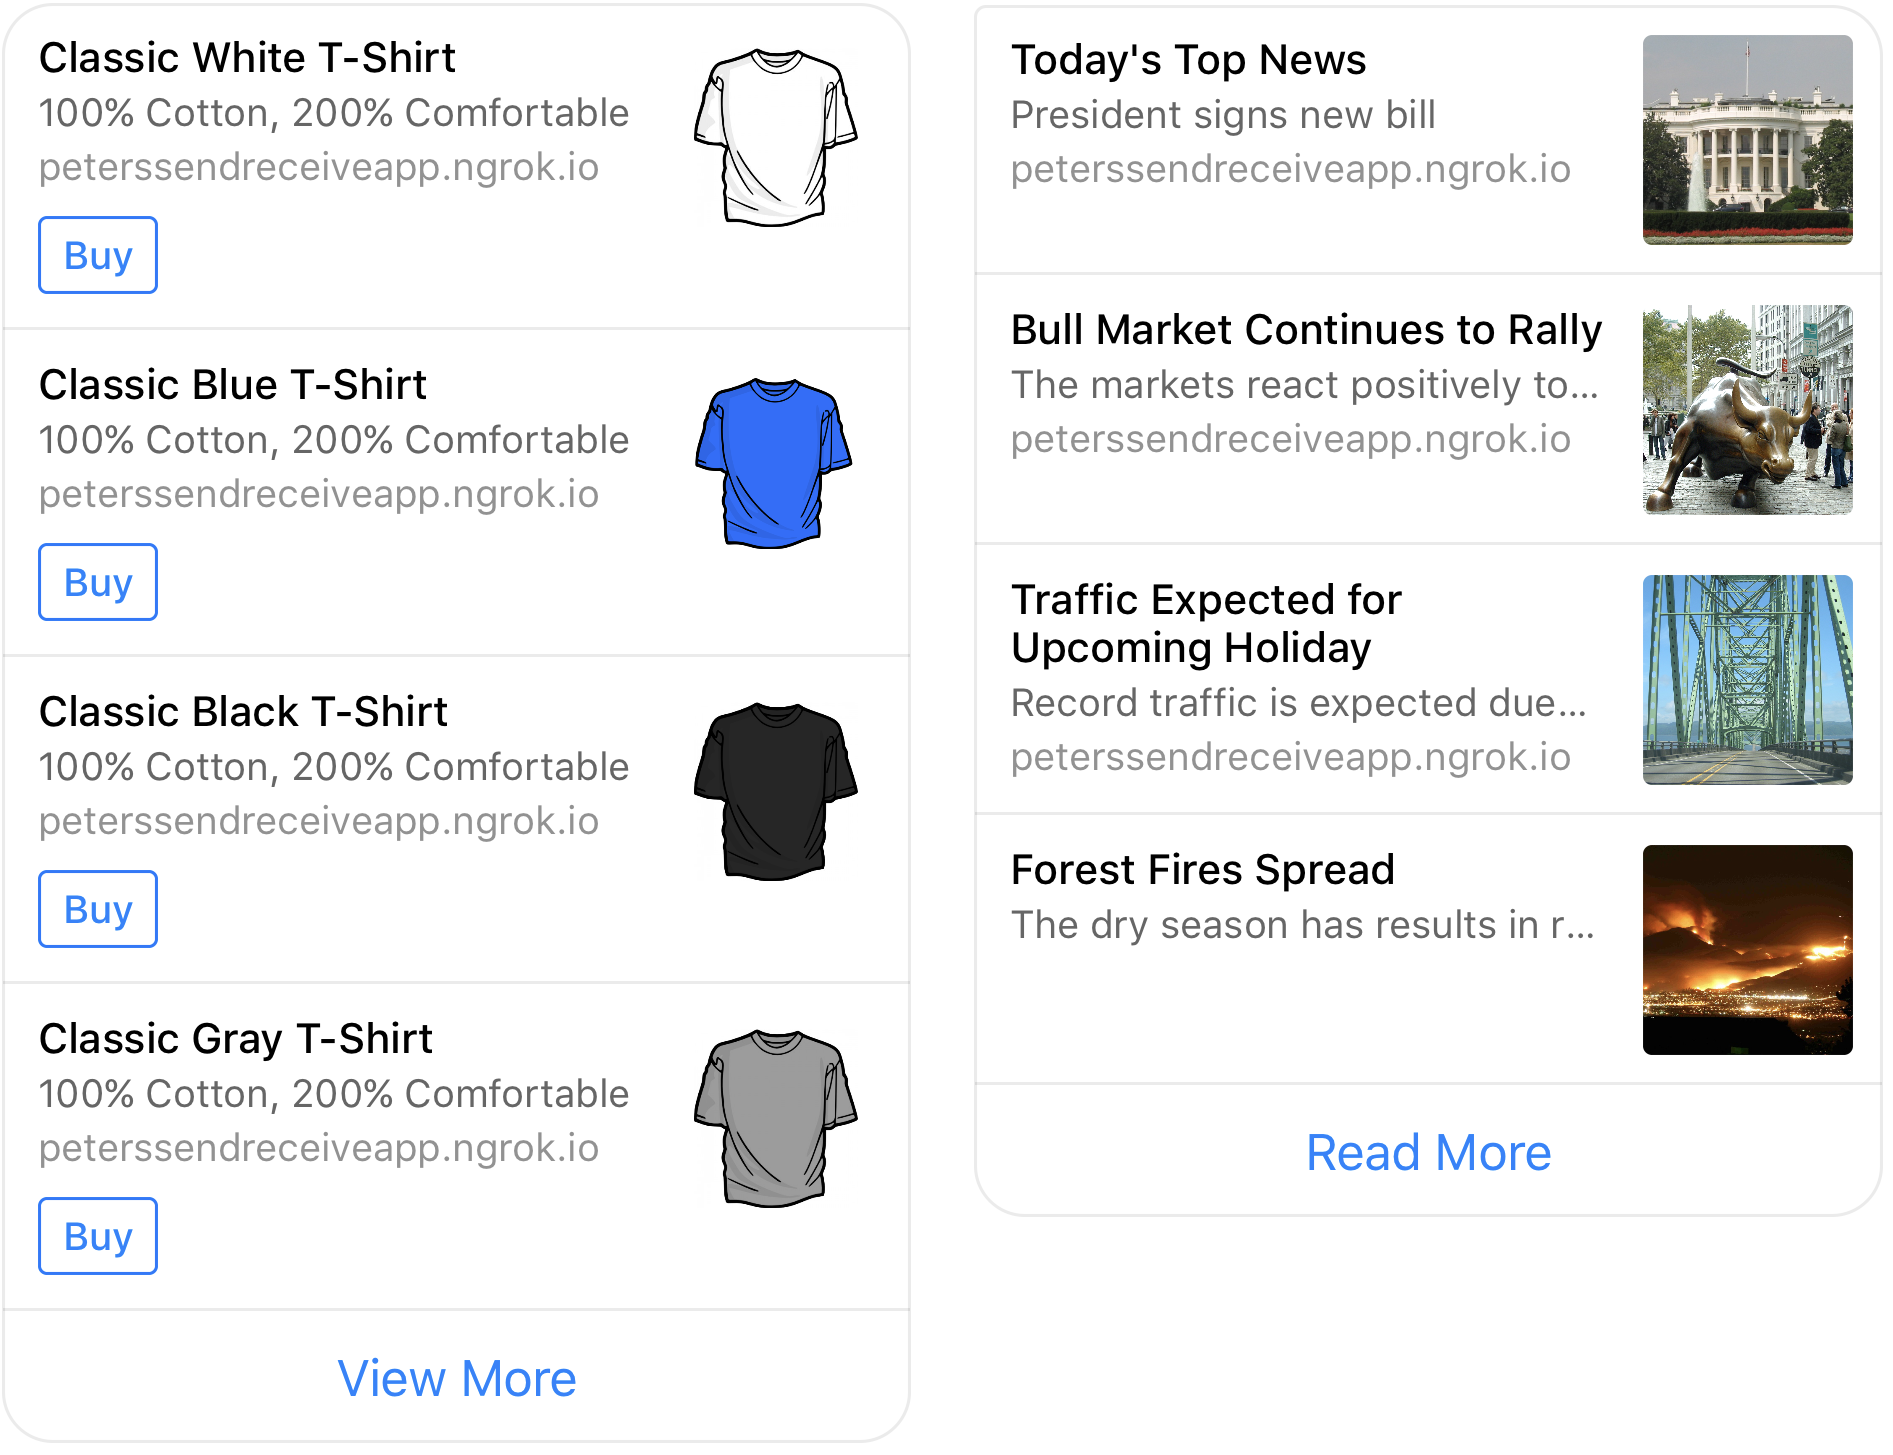
\includegraphics[scale=0.2]{../Immagini/modello_lista.png}
	\caption{Modello generico di carosello per Facebook Messenger}
\end{figure}
\newpage
Il compito assegnato allo stagista è stato quello di integrare questo meccanismo in due diversi \gls{Chatbot} creati dall'azienda:
\begin{itemize}
	\item \textbf{gestore eventi}: è un applicativo creato da \azienda{} per essere utilizzato durante lo svolgimento di eventi della durata di uno o più giornate. Attraverso questo \gls{Chatbot} l'utente può recuperare delle informazione riguardanti le conferenze in programma, le aule disponibili e le giornate dell'evento;
	\item \textbf{meteo Veneto bot}\footcite{meteo}: questo \gls{Chatbot} utilizza i dati di ARPA Veneto\footcite{arpav} per mostrare le previsioni del tempo del Veneto;
\end{itemize}
Il progetto si divideva quindi in tre parti:
\begin{itemize}
	\item analisi preliminare degli \gls{SDK} delle principali piattaforme per il \gls{NLP} presenti sul mercato, in modo da valutarne pregi e difetti;
	\item creazione della logica per la gestione delle domande utente all'interno della piattaforma scelta;
	\item integrazione di questa nuova funzionalità nel software utilizzato da \azienda{} per la gestione dei \gls{Chatbot}. 
\end{itemize}
Visto il bisogno di un periodo iniziale di studio, sia per capire le possibilità e i limiti degli strumenti da dover utilizzare nella trasformazione delle \gls{FAQ} in dati processabili, sia per apprenderne a pieno il funzionamento tramite la documentazione presente, \azienda{} ha ritenuto questo progetto idoneo ad uno studente universitario, il quale ha a disposizione circa 300 ore per formarsi su tutto ciò di cui vi è bisogno, e successivamente portare a termine il prodotto richiesto.

\section{Modalità di svolgimento}
Per quanto riguarda lo svolgimento dello stage è stato deciso di comune accordo che dovesse essere svolto nella sede dell'azienda. Questa decisione mi ha permesso di confrontarmi con personale più esperto, un ambiente nuovo e stimolante e con la vera realtà del mondo del lavoro. Tutti i membri dell'azienda, compreso il tutor, si sono rivelati molto disponibili alle mie richieste di chiarimento su alcuni aspetti dello sviluppo e della gestione del progetto.\\
Durante la creazione del prodotto sono state mostrate le nuove funzionalità a tutto il team aziendale, in modo da discuterne pregi, difetti e possibili miglioramenti. \\
L'orario lavorativo è stato il seguente: da lunedì a venerdì, dalle 8:00 alle 12:00 e dalle 14:00 alle 18:00.

\section{Obiettivi dello stage}
\label{obiettivi}
Prima di iniziare il periodo di stage, sono stati delineati i seguenti obiettivi, divisi in base alla loro importanza: obbligatori o desiderabili.

\subsection{Obiettivi obbligatori}
\begin{itemize}
	\item analisi del problema e studio delle possibili soluzioni già esistenti nel mercato;
	\item analisi e confronto delle piattaforme per il \gls{NLP};
	\item progettazione delle categorie di domande che la piattaforma deve gestire;
	\item sviluppo client di prova integrato tramite la piattaforma di \gls{NLP};
	\item sviluppo dell'integrazione della piattaforma con Facebook Messenger.
\end{itemize}

\subsection{Obiettivi desiderabili}
\begin{itemize}
	\item test e monitoraggio dell’applicativo tramite l’integrazione con 2 pagine Facebook reali;
\end{itemize}

\section{Pianificazione del lavoro}
Prima del periodo di stage è stato pianificato, insieme al tutor aziendale, il lavoro da svolgere su base settimanale. Questa suddivisione prevede:
\begin{itemize}
	\item \textbf{prima settimana}: analisi preliminare del problema e verifica delle soluzioni attualmente disponibili sul mercato;
	\item \textbf{seconda settimana}: analisi delle piattaforme di \gls{NLP} presenti sul mercato;
	\item \textbf{terza settimana}: analisi dei requisiti da soddisfare nello sviluppo del prodotto;
	\item \textbf{quarta settimana}: progettazione della piattaforma scelta e dell'integrazione nel software aziendale;
	\item \textbf{quinta e sesta settimana}: istruzione della piattaforma per il \gls{NLP} per entrambi i \gls{Chatbot}, con la relativa integrazione nel software aziendale;
	\item \textbf{settimana settimana}: \emph{testing} delle funzionalità attraverso 2 pagine di Facebook reali;
\end{itemize}

La figura \ref{gantt} mostra la pianificazione del lavoro attraverso un \gls{Diagramma di gantt}.
\begin{figure}[h]
	\centering
	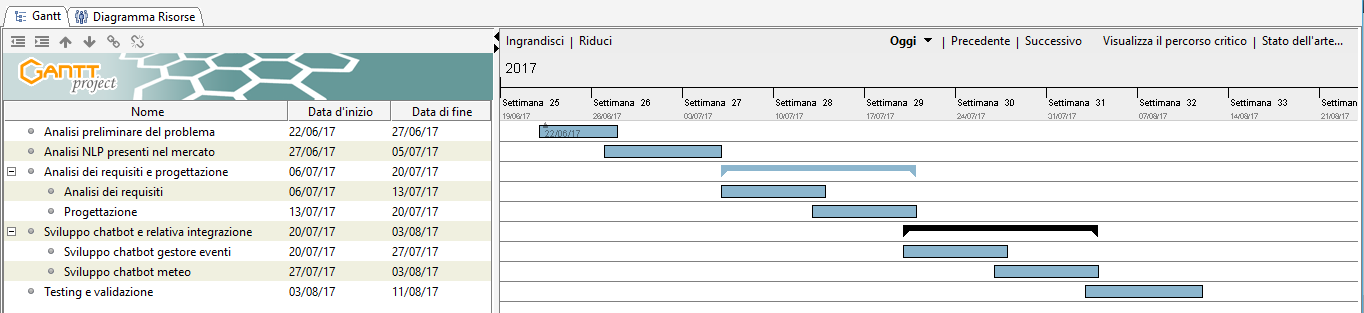
\includegraphics[scale=0.4]{../Immagini/gantt.png}
	\caption{Diagramma di Gantt}\label{gantt}
\end{figure}

\section{Principali problematiche}
Durante il periodo di stage, sono state incontrare diverse difficoltà, utili a migliorare la capacità di scelta e decisione dello stagista, ma anche la comunicazione e il lavoro all'interno di un team.

\subsection{Difficoltà di ambientazione}
Nei primi giorni in azienda l'ostacolo principale è stato l'inserimento in un team di lavoro affiatato e di esperienza, nonostante i suoi componenti siano stati molto disponibili e aperti a domande e chiarimenti. In particolare:
\begin{itemize}
	\item il \textbf{linguaggio tecnico/aziendale} non è stato da subito di facile apprendimento. In parte il problema sorgeva quando i \glspl{Brainstorming} del team vertevano su tecnologie a me sconosciute, oppure su aspetti tecnici dei loro prodotti. Con il passare del tempo, attraverso l'utilizzo di un piccolo glossario individuale dove segnavo le spiegazioni dei termini a me non chiari, ho assimilato la maggior parte dei concetti, potendo così partecipare alle riunione del team in modo attivo e costruttivo;
	\item lavorare all'interno di un \textbf{team} non è un'attività semplice. Bisogna imparare a rispettare le scadenze nel rispetto dei colleghi e saper elaborare strategie nel caso in cui essi non siano riusciti a rispettare le proprie. Grazie all'esperienza che ho maturato sotto questo punto di vista, ho capito quanto sia importante pianificare con cura le attività e il tempo da destinare ad ognuna di esse.
\end{itemize}

\subsection{Difficoltà lavorative e soluzioni adottate}
Durante lo svolgimento del mio progetto ho riscontrato queste difficoltà principali:
\begin{itemize}
	\item scelta del \textbf{miglior strumento per il \gls{NLP}}: il \gls{NLP} è un problema che è stato affrontato relativamente recentemente nel mondo dell'informatica. Le tecnologie che il mercato mette a disposizione sono limitate e spesso non soddisfacenti per gli obiettivi che mi sono stati richiesti. La ricerca di uno strumento idoneo non è stata facile, anche perchè l'azienda richiedeva non ci fossero costi per il suo utilizzo. Dopo una buona analisi del mercato, con la produzione di una relativa documentazione consegnata al tutor aziendale, è stato deciso di utilizzare api.ai, servizio acquistato da Google nel 2016, che offre svariate funzionalità senza alcun costo, ma con delle sole limitazioni in termini di richieste giornaliere e mensili (una breve analisi dei principali strumenti di NLP è presente nella sezione \ref{nlp});
	\item \textbf{possibili richieste degli utenti}: il mio compito era quello di fornire una risposta tramite i \glspl{Chatbot} alle possibile domande di un utilizzatore. Se in primo momento questo non sembrava un \emph{task} troppo complicato, si è però trasformato in un problema non di semplice gestione, in quanto il dominio di richieste di un utente può essere vasto e molto vario. Per cercare di superare questo ostacolo, in accordo con il tutor e il team aziendale, si è deciso di limitare le categorie di domande a cui il \gls{Chatbot} risponde, fornendo un messaggio adeguato in caso di una richiesta dell'utente non gestita. Sarà poi compito dell'azienda ampliare le funzionalità dei \glspl{Chatbot}, visto il poco tempo a mia disposizione, valutando le richieste fatte dagli utenti nell'apposita sezione di Api.ai;
	\item \textbf{gestione del sessionId}: nel \gls{JSON} utilizzato per interrogare api.ai tramite una richiesta \gls{POST}, deve essere presente obbligatoriamente il campo \textbf{sessionId}, per identificare univocamente il mittente della richiesta. La gestione di questo campo è stata quindi di notevole importanza nel garantire ad ogni utente una corretta interazione con il \gls{Chatbot}. Per assegnare ad ogni utente un sessionId univoco è stato deciso di creare un campo nella tabella degli utenti del database, dove memorizzare la stringa rappresentata dall'id dell'utente nel database e il \emph{timestamp} del momento in cui esso si è collegato al bot, garantendo così l'unicità della stessa. In questo modo api.ai, e di conseguenza il \gls{Chatbot}, gestiscono tutti i possibili utenti separatamente e non come un'unica persona;
	\item \textbf{documentazione scarsa del software aziendale}: dopo aver istruito la piattaforma di api.ai, avevo il compito di integrare le nuove funzionalità nel software aziendale dedicato alla gestione dei \glspl{Chatbot}. Il problema è sorto quando non ho avuto a disposizione una chiara documentazione del codice, in modo da capirne \emph{package}, classi e metodi. Per risolvere questa mancanza ho chiesto al mio tutor aziendale una breve spiegazione delle porzioni di codice che avrei dovuto riutilizzare nelle mie nuove classi, potendo così capire il funzionamento generale dei vari \emph{package}. Grazie al mio studio individuale, e alcuni chiarimenti chiesti agli sviluppatori, ho potuto passare autonomamente all'attività di programmazione, introducendo così le mie nuove funzionalità del prodotto.
\end{itemize}

\section{Strumenti utilizzati}
\subsection{NetBeans}
NetBeans è un ambiente di sviluppo integrato multi-linguaggio, nato nel giugno 2000 e scritto interamente in Java, scelto dalla Oracle Corporation come \gls{IDE} ufficiale da contrapporre al più diffuso Eclipse.
L'azienda non ha posto nessun vincolo sull'ambiente di sviluppo da adottare, così come vale per i propri dipendenti. Ho deciso di utilizzare NetBeans in quanto è molto intuitivo e di semplice utilizzo.\\
Inoltre offre una integrazione con \gls{Mercurial} per gestire \emph{push}, \emph{pull} e \emph{commit} senza utilizzare le righe di comando.
\begin{figure}[h]
	\centering
	
\includegraphics[scale=0.4]{../Immagini/netbeans.jpg}
	\caption{Logo di NetBeans}
\end{figure}
\subsection{Api.ai}
Api.ai è una società nata nell'ottobre del 2010 e acquisita da Google Inc. nel 2016. Api.ai è una piattaforma di conversazione
che permette interazioni sofisticate con il linguaggio naturale. All'interno del progetto è stata utilizzata per trasformare le domande degli utenti in dati processabili, dopo aver creato due \emph{agents}, uno per ciascun \gls{Chatbot}, ed averli istruiti secondo le possibili \gls{FAQ} dei rispettivi ambiti di utilizzo.\\
Api.ai poteva essere integrato nel software aziendale in due diversi modi:
\begin{itemize}
	\item \textbf{connesso direttamente al \gls{Chatbot}} di Facebook Messenger, grazie alla semplice integrazione prevista da api.ai, estraendo le informazioni dal database aziendale tramite dei \emph{webhook}, anch'essi facilmente gestibili tramite la piattaforma di api.ai;
	\item come \textbf{strumento esterno} al software aziendale, con il bisogno di interrogarlo tramite delle richieste \gls{POST} HTTP solo in alcuni casi specifici, con le domande poste dall'utente.
\end{itemize} 
Dopo aver valutato entrambe le opzioni, ho scelto di intraprendere la seconda per due motivazioni:
\begin{itemize}
	\item utilizzando api.ai come strumento esterno non è stato necessario introdurre dipendenze verso di esso nel codice, dando così la possibilità, se ci fosse bisogno in futuro, all'azienda di cambiare questa tecnologia con un'altra senza grossi problemi, cosa che sarebbe stata molto più difficile nell'altro caso;
	\item api.ai mette a disposizione un \gls{SDK} per Java molto utile, anche se non ben documentato. In ogni caso dopo aver capito il suo funzionamento è stato semplice sfruttarlo per interrogare api.ai con poche righe di codice. 
\end{itemize}
\begin{figure}[h]
	\centering
	
\includegraphics[scale=0.2]{../Immagini/apiai.png}
	\caption{Logo di api.ai}
\end{figure}
\subsection{Hibernate}
Hibernate è una piattaforma \gls{Open source} ad alto rendimento per lo sviluppo di applicazioni Java, che fornisce il servizio di \gls{ORM}, ovvero si occupa della mappatura tra le classi Java e le relative tabelle di un database \gls{SQL}.
Gestisce dunque il salvataggio degli oggetti di tali classi ed il reperimento dalle entità dal database, automatizzando le \emph{query} necessarie e provvedendo alla reistanziazione dell’oggetto mappato sul database.
\begin{figure}[h]
	\centering
	
\includegraphics[scale=0.35]{../Immagini/Hibernate.png}
	\caption{Logo di Hibernate}
\end{figure}

\subsection{Database MySQL} 
L'azienda \azienda{} utilizza un database MySQL per la memorizzazione e gestione dei dati relativi ai progetti dei \glspl{Chatbot}. È il più diffuso database \gls{Open source} basato sul linguaggio \gls{SQL} ed è di tipo relazionale, ovvero segue il principio che tutti i dati sono rappresentati come relazioni e manipolati con gli operatori dell’algebra relazionale o del calcolo relazionale.
Lo stagista è stato incaricato di capirne la struttura e come esso veniva gestito all'interno dell'applicativo, per poi utilizzarlo al meglio nello sviluppo del proprio prodotto.\\

\subsection{Strumenti aziendali}
Infine sono stati utilizzati alcuni degli strumenti consolidati nel contesto aziendale, come \textbf{BitBucket} e \gls{Mercurial} per quanto riguarda il versionamento del codice, \textbf{Slack} per le comunicazioni con gli altri dipendenti e il tutor ed \textbf{Asana} per il tracciamento dei \emph{task} da svolgere (strumenti esposti nella sezione \ref{Tecnologie}).



\section{Prodotto ottenuto}
Il prodotto che mi è stato richiesto di sviluppare consisteva in un incremento delle funzionalità di due \glspl{Chatbot}, creati e gestiti da \azienda{}, per offrire agli utenti uno strumento che si avvicinasse il più possibile ad una chat normale con un essere umano.\\
Al mio arrivo in azienda questi due prodotti potevano essere utilizzati dagli utenti solamente attraverso l'interfaccia grafica che mettono a disposizione. In particolare, per i \gls{Chatbot} di Facebook Messenger è possibile creare un menù, usufruibile in qualsiasi momento attraverso il pulsante rappresentato dalle 3 righe orizzontali, dove inserire dei comandi per mostrare determinate categorie di informazioni (ad esempio nel bot per le previsioni del tempo esiste il comando "Previsioni" che mostra il meteo per tutta la settimana, nella zona di interesse). 
\begin{figure}[!h]
	\centering
	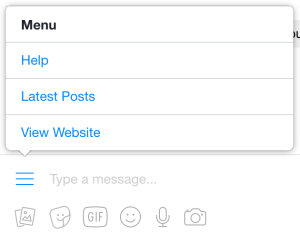
\includegraphics[scale=0.6]{../Immagini/menu.png}
	\caption{Esempio di menù di un \gls{Chatbot} di Facebook}
\end{figure}

Ci sono poi altri "caroselli" messi a disposizione dello sviluppatore per costruire le proprie risposte, spiegati ed illustrati nella documentazione di Messenger-platform\footcite{messenger}.\\

I risultati che sono riuscito ad ottenere nelle 300 ore di stage sono stati ritenuti molto soddisfacenti dall'azienda, che utilizza già le mie funzionalità nel bot del meteo. Gli incrementi che ho apportato ai due \glspl{Chatbot} sono esposti di seguito. 

\subsubsection{Meteo Veneto Bot}
Si tratta di un \gls{Chatbot} innovativo che sfrutta i dati messi a disposizione da ARPA Veneto attraverso un file \gls{Extensible Markup Language}. Il compito di questo  \gls{Chatbot} è di dare delle informazioni all'utente sulle previsioni del tempo nella regione del Veneto, in particolare nella zona di interesse dell'utente che specifica all'inizio della conversazione inviando la propria posizione, o scrivendo il comune che desidera. Dopo aver premuto il pulsante "Previsioni", presente nel menù, si possono visualizzare i dettagli del meteo dei vari giorni della settimana, che mostrano temperature, precipitazione, venti ed ascoltare il bollettino.\\
Al termine del mio lavoro sono state introdotte nuove funzionalità che permettono all'utente di domandare:
\begin{itemize}
	\item il meteo per un determinato giorno in un comune preciso;
	\item se è prevista pioggia, neve, sole, nebbia per un determinato giorno in un comune preciso;
	\item le temperature previste;
	\item di ascoltare il bollettino emesso da ARPA Veneto.
\end{itemize}

\subsubsection{Gestore di eventi}
Si tratta di un template di \gls{Chatbot} sviluppato da \azienda{} che viene  personalizzato ogni qualvolta un cliente ne richieda l'utilizzo, mantenendo in ogni caso delle funzionalità principali. Il suo compito è quello di mostrare delle informazioni riguardanti l'evento per il quale il \gls{Chatbot} è stato personalizzato. In particolare si possono ottenere delle indicazioni sulle conferenze, come orario, durata, argomento, e sulle sale presenti.\\
Il mio compito in questo caso era di rendere queste funzionalità di immediato utilizzo attraverso delle domande da chiedere al bot. Adesso è possibile chiedere:
\begin{itemize}
	\item in \textbf{generale}:
	\begin{itemize}
		\item il programma dell'evento, specificando giorno ora e sala (non obbligatoriamente tutti e tre);
	\end{itemize}
	\item per le \textbf{conferenze}:
	\begin{itemize}
		\item la durata;
		\item l'orario di inizio e fine;
		\item in che sala si svolge;
	\end{itemize}
	\item per le \textbf{sale}:
	\begin{itemize}
		\item le indicazioni per trovarla;
		\item quale conferenza si svolge in un determinato giorno e orario;
		\item la conferenza successiva a quella in corso;
	\end{itemize}
\end{itemize}

Una volta posta una domanda al \gls{Chatbot}, e ricevuta la relativa risposta, è stato anche implementato un sistema che permette all'utente di fare lo stesso tipo di domanda, come se stesse colloquiando con un essere umano. Ad esempio:

\begin{itemize}
	\item[-] Utente: "Che conferenza si svolge alle 12 in Lum250?"
	\item[-] Bot: "Analisi matematica"
	\item[-] Utente: "E in P140?"
	\item[-] Bot: "Programmazione 1".
\end{itemize}
Nella seconda risposta il sistema ha tenuto conto della prima domanda fatta dall'utente, cercando così la conferenza che si svolge alle 12 in P140. Questo meccanismo è stato implementato grazie ai \emph{context} di api.ai.

             % Descrizione progetto
% !TEX encoding = UTF-8
% !TEX TS-program = pdflatex
% !TEX root = ../tesi.tex

%**************************************************************
\chapter{Analisi dei requisiti}
\label{cap:analisi}

Il primo giorno di stage il tutor aziendale ha indetto una riunione con tutti i dipendenti per definire le funzionalità del prodotto che dovevo sviluppare. Attraverso questo \gls{Brainstorming} ho potuto farmi un'idea più precisa del compito a me assegnato. Una volta terminata l'analisi degli strumenti per il \gls{NLP}, ho potuto svolgere l'analisi dei requisiti del mio prodotto. In accordo con il tutor non ho dovuto stilare un documento formale che comprendesse i casi d'uso, ma solo una lista di requisiti funzionali che il prodotto avrebbe dovuto soddisfare.

\section{Tracciamento dei requisiti}
\label{requisiti}
Nella tabella che seguono verranno presentati i principali requisiti individuati durante l’analisi del problema.
Ogni requisito individuato avrà un codice identificativo univoco così formato: \\
\centerline{R\{Importanza\}\{Codice\}} \\ 
dove:
\begin{itemize}
	\item \textbf{importanza} può assumere uno dei seguenti valori:
	\begin{itemize}
		\item \textbf{O}: indica un requisito obbligatorio;
		\item \textbf{D}: indica un requisito desiderabile;
	\end{itemize}
	\item \textbf{codice} indica il codice identificativo del requisito, è univoco e deve essere
identificato in forma gerarchica.
\end{itemize}

La prima tabella contiene i requisiti comuni ai due \gls{Chatbot} oggetti dello stage, la seconda tabella riporta i requisiti specifici del \gls{Chatbot} per la gestione degli eventi, mentre la terza quelli di Meteo Veneto bot.
\newpage
\normalsize
\begin{longtable}{|c|>{\centering}m{7cm}|c|}
\hline
\textbf{Id Requisito} & \textbf{Descrizione} & \textbf{Importanza}\\
\hline
\endhead
RO1 & L'utente deve poter interagire con il sistema attraverso delle domande di senso compiuto & Obbligatorio\\ 
RO2 & Il sistema deve permettere all'utente di interagire con esso nel modo più naturale possibile & Obbligatorio \\
RD3 & Il sistema deve rispondere all'utente sfruttando i modelli messi a disposizione da Facebook Messenger & Desiderabile\\
RD4 & Il sistema deve fornire all'utente un messaggio idoneo, nel caso di una domanda non gestibile & Obbligatorio\\
\hline
\caption{Requisiti funzionali generali}
\end{longtable}

\normalsize
\begin{longtable}{|c|>{\centering}m{7cm}|c|}
\hline
\textbf{Id Requisito} & \textbf{Descrizione} & \textbf{Importanza}\\
\hline
\endhead
RO1.1 & L'utente deve poter chiedere informazioni riguardo una conferenza & Obbligatorio\\ 
RO1.1.1 & L'utente deve poter chiedere l'orario di inizio e fine di una conferenza & Obbligatorio\\ 
RO1.1.2 & L'utente deve poter chiedere la durata di una conferenza & Obbligatorio\\
RO1.1.3 & L'utente deve poter chiedere in che aula si svolge la conferenza & Obbligatorio\\  
RO1.2 & L'utente deve poter chiedere informazioni riguardo le aule dell'evento & Obbligatorio\\ 
RO1.2.1 & L'utente deve poter chiedere delle indicazioni per raggiungere un'aula & Obbligatorio\\ 
RO1.3 & L'utente deve poter chiedere informazioni riguardo il programma dell'evento & Obbligatorio\\ 
RO1.3.1 & L'utente deve poter chiedere informazioni riguardo il programma dell'evento in una specifica giornata & Obbligatorio\\ 
RO1.3.2 & L'utente deve poter chiedere informazioni riguardo il programma dell'evento in una specifica giornata ed in una precisa stanza & Obbligatorio\\
RO1.3.3 & L'utente deve poter chiedere informazioni riguardo il programma dell'evento in una specifica ora ed in una precisa stanza & Obbligatorio\\
RO1.3.4 & L'utente deve poter chiedere informazioni riguardo il programma dell'evento specificando il giorno, l'ora e l'aula & Obbligatorio\\
RD5 & L'utente deve poter ricevere informazioni sul funzionamento del \gls{Chatbot} scrivendo "aiuto" & Desiderabile\\ 
RO6 & L'utente deve poter visualizzare la propria agenda scrivendo "agenda" & Obbligatorio\\ 
\hline
\caption{Requisiti funzionali del chatbot per la gestione degli eventi}
\end{longtable}

\normalsize
\begin{longtable}{|c|>{\centering}m{7cm}|c|}
\hline
\textbf{Id Requisito} & \textbf{Descrizione} & \textbf{Importanza}\\
\hline
\endhead
RO1.4 & L'utente deve poter chiedere le previsioni del meteo & Obbligatorio\\ 
RO1.4.1 & L'utente deve poter chiedere le previsioni del meteo in un determinato comune del Veneto & Obbligatorio\\
RO1.4.2 & L'utente deve poter chiedere le previsioni del meteo per un determinato giorno o periodo di tempo(es. weekend) & Obbligatorio\\  
RO1.4.3 & L'utente deve poter chiedere le previsioni del meteo per un determinato giorno o periodo di tempo(es. wweekend), in un preciso comune del Veneto & Obbligatorio\\ 
RO1.5 & L'utente deve poter chiedere le temperature previste & Obbligatorio\\ 
RO1.5.1 & L'utente deve poter chiedere le temperature previste in un determinato giorno o periodo di tempo & Obbligatorio\\
RO1.5.2 & L'utente deve poter chiedere le temperature previste in un determinato comune del Veneto & Obbligatorio\\  
RO1.5.3 & L'utente deve poter chiedere le temperature previste in un determinato comune del Veneto, per uno specifico giorno o periodo di tempo & Obbligatorio\\ 
RO1.6 & L'utente deve poter chiedere se è previsto il sole & Obbligatorio\\ 
RO1.6.1 & L'utente deve poter chiedere se è previsto il sole in un determinato giorno o periodo di tempo & Obbligatorio\\
RO1.6.2 & L'utente deve poter chiedere le se è previsto il sole in un determinato comune del Veneto & Obbligatorio\\  
RO1.6.3 & L'utente deve poter chiedere se è previsto il sole in un determinato comune del Veneto, per uno specifico giorno o periodo di tempo & Obbligatorio\\  
RO1.7 & L'utente deve poter chiedere se è prevista pioggia & Obbligatorio\\ 
RO1.7.1 & L'utente deve poter chiedere se è prevista pioggia in un determinato giorno o periodo di tempo & Obbligatorio\\
RO1.7.2 & L'utente deve poter chiedere le se è prevista pioggia in un determinato comune del Veneto & Obbligatorio\\  
RO1.7.3 & L'utente deve poter chiedere se è prevista pioggia in un determinato comune del Veneto, per uno specifico giorno o periodo di tempo & Obbligatorio\\ 
RO1.8 & L'utente deve poter chiedere se è prevista neve & Obbligatorio\\ 
RO1.8.1 & L'utente deve poter chiedere se è prevista neve in un determinato giorno o periodo di tempo & Obbligatorio\\
RO1.8.2 & L'utente deve poter chiedere le se è prevista neve in un determinato comune del Veneto & Obbligatorio\\  
RO1.8.3 & L'utente deve poter chiedere se è prevista neve in un determinato comune del Veneto, per uno specifico giorno o periodo di tempo & Obbligatorio\\ 
RD1.9 & L'utente deve poter chiedere se è previsto bel tempo & Obbligatorio\\ 
RD1.9.1 & L'utente deve poter chiedere se è previsto bel tempo in un determinato giorno o periodo di tempo & Desiderabile\\
RD1.9.2 & L'utente deve poter chiedere le se è previsto bel tempo in un determinato comune del Veneto & Obbligatorio\\  
RD1.9.3 & L'utente deve poter chiedere se è previsto brutto tempo in un determinato comune del Veneto, per uno specifico giorno o periodo di tempo & Obbligatorio\\ 
RD1.10 & L'utente deve poter chiedere se è previsto brutto tempo & Obbligatorio\\ 
RD1.10.1 & L'utente deve poter chiedere se è previsto brutto tempo in un determinato giorno o periodo di tempo & Desiderabile\\
RD1.10.2 & L'utente deve poter chiedere le se è previsto brutto tempo in un determinato comune del Veneto & Obbligatorio\\  
RO1.10.3 & L'utente deve poter chiedere se è previsto brutto tempo in un determinato comune del Veneto, per uno specifico giorno o periodo di tempo & Obbligatorio\\ 
RO1.11 & L'utente deve poter chiedere se è prevista nebbia tempo & Obbligatorio\\ 
RO1.11.1 & L'utente deve poter chiedere se è prevista nebbia tempo in un determinato giorno o periodo di tempo & Desiderabile\\
RO1.11.2 & L'utente deve poter chiedere le se è prevista nebbia tempo in un determinato comune del Veneto & Obbligatorio\\  
RD1.11.3 & L'utente deve poter chiedere se è prevista nebbia tempo in un determinato comune del Veneto, per uno specifico giorno o periodo di tempo & Obbligatorio\\ 
RO1.12 & L'utente deve poter chiedere se sono presenti fenomeni particolari o avvisi speciali & Obbligatorio\\ 
RO7 & Il sistema deve fornire le informazioni del comune in cui l'utente si è registrato, nel caso non ne specifichi un altro nella domanda & Obbligatorio\\
RO8 & L'utente deve poter riceve l'audio del bollettino meteo scrivendo "ascolta bollettino" & Obbligatorio\\ 
\hline
\caption{Requisiti funzionali del chatbot Meteo Veneto Bot}
\end{longtable}

\section{Analisi di mercato}
\label{nlp}
Il primo passo da compiere per iniziare lo sviluppo de prodotto è stato scegliere la piattaforma di \gls{NLP} migliore in base ai requisiti imposti dall'azienda. Le richieste fatte da \azienda{} riguardanti questo strumento erano le seguenti:
\begin{itemize}
	\item \textbf{costo}: il prezzo per il suo utilizzo doveva essere uguale a 0;
	\item \textbf{lingua}: deve supportare la lingua italiana, visto che al momento attuale i \glspl{Chatbot} sono implementati solo con quella;
	\item \textbf{documentazione}: il servizio deve essere ben documentato per permettere all'azienda, una volta finito il periodo di stage, di imparare ad utilizzarlo velocemente.
\end{itemize}

Questa attività di analisi di mercato si è rivelata quindi fondamentale per la buona riuscita del progetto, visto l'importanza che questo strumento avrebbe avuto nell'intero periodo di sviluppo. Le piattaforme da me studiate e analizzate sono riportate di seguito.

\subsubsection{IBM Watson Conversation}
IBM Watson Conversation\footcite{watson} è un prodotto della piattaforma IBM Watson, che attraverso IBM Cloud dà la possibilità di integrare i più potenti mezzi di \gls{AI} nelle tue applicazioni. Il servizio di Conversation, oltre alla possibilità di creare \gls{Chatbot} e agenti virtuali, può essere istruito ed interrogato per analizzare il testo posto in input, attraverso le \gls{API} messe a disposizione.\\
È possibile infatti creare dei \emph{workspace} dedicati dove, attraverso \emph{intent} ed \emph{entities} creati e gestiti dallo sviluppatore, analizzare le domande poste dagli utenti, estraendo i dati che più interessano. L'integrazione con l'applicativo aziendale risultava semplice, grazie al \gls{SDK} di Java\footcite{watsonSDK} messo a disposizione da IBM.

\begin{figure}[h]
	\centering
	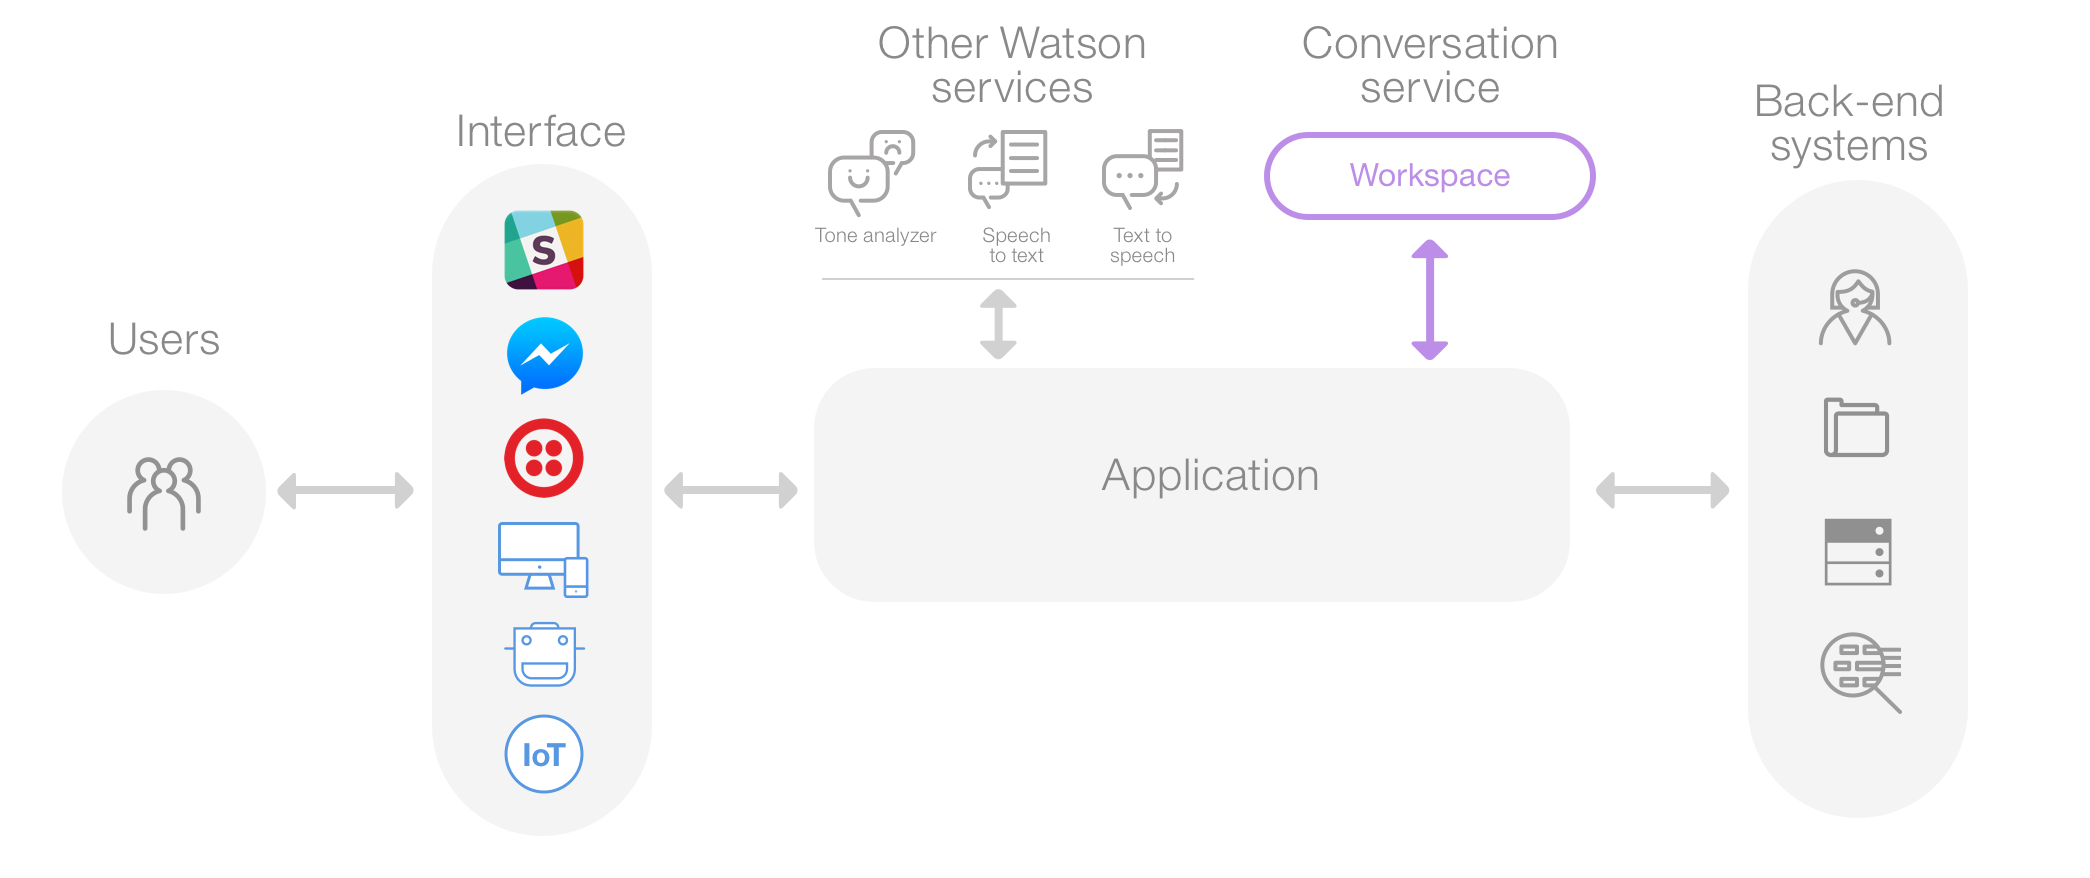
\includegraphics[scale=0.15]{../Immagini/conversation_arch_overview.png}
	\caption{Funzionamento IBM Watson Converation}
\end{figure}

Per quanto riguarda le richieste dell'azienda:
\begin{itemize}
	\item la \textbf{lingua italiana} è supportata, e non in versione beta;
	\item la \textbf{documentazione} è chiara ed esaustiva, con dei video di esempio molto utili;
	\item esiste un piano di \textbf{costi} gratis, chiamato \emph{Lite}, che però dà la possibilità di creare un numero limitato di \emph{workspace}, \emph{intent} ed \emph{entity}, risultando troppo vincolante per i futuri utilizzi aziendali. Le soluzioni a pagamento non sono state prese in considerazione in quanto non percorribili per l'azienda, almeno in un primo momento di utilizzo di questi servizi.
\end{itemize}

\begin{figure}[h]
	\centering
	
\includegraphics[scale=0.1]{../Immagini/watson_conversations_icon.png}
	\caption{Logo di IBM Watson Conversation}
\end{figure}

\subsubsection{wit.ai}
wit.ai\footcite{witai} è una società nata nell'ottobre del 2013 e acquisita da Facebook Inc. nel 2015.
L'obiettivo di wit.ai è quello di semplificare la creazione di applicazioni che prevedono interazioni testuali o vocali; per farlo viene messa a disposizione degli sviluppatori una piattaforma di linguaggio naturale aperta ed estensibile che ha la peculiarità di apprendere tramite ogni interazione eseguita.\\
wit.ai mette a disposizione un \gls{SDK} gratuito ed \gls{Open source} per il riconoscimento del linguaggio
naturale. Questa piattaforma è caratterizzata dall'utilizzo di \emph{context}, \emph{intent} ed \emph{entity} che sono
dei costrutti messi a disposizione per tradurre le richieste vocali dell'utente in dati processabili. In particolare il \emph{context} si utilizza per monitorare lo stato della conversazione tra l'utente e wit.ai.

\begin{figure}[h]
	\centering
	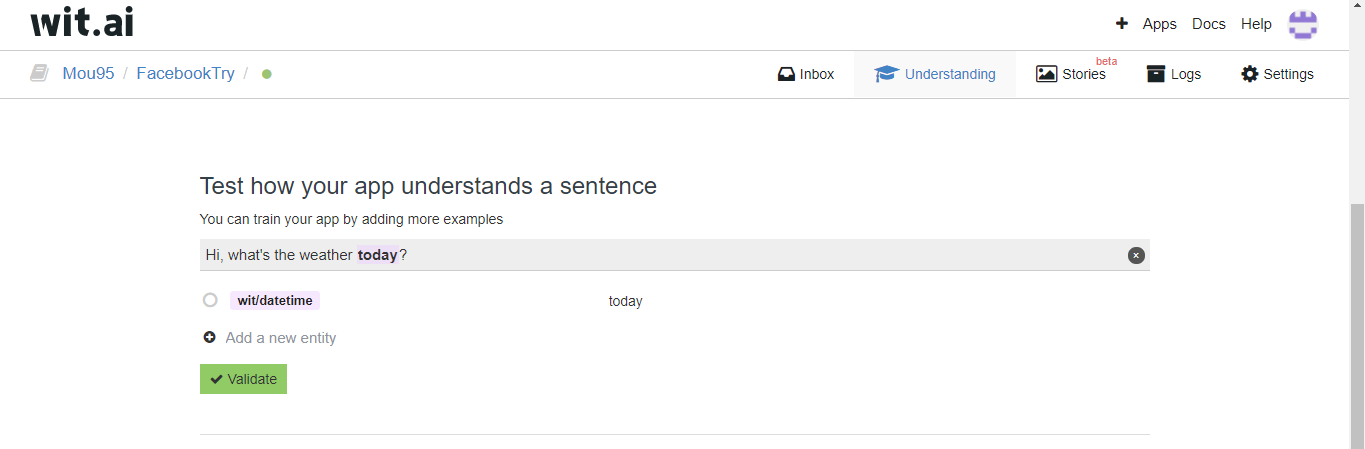
\includegraphics[scale=0.4]{../Immagini/witai_example.png}
	\caption{Esempio di creazione di un intent in wit.ai}
\end{figure}

Per quanto riguarda le richieste dell'azienda:
\begin{itemize}
	\item la \textbf{lingua italiana} è supportata;
	\item la \textbf{documentazione} è chiara ed esaustiva;
	\item l'utilizzo di wit.ai è completamente \textbf{gratuito} per progetti sia pubblici che privati.
\end{itemize}

Dal punto di vista tecnico l'unica mancanza di questo strumento, che ha influito nella decisione di non adottarlo, è la impossibilità di impostare delle \emph{required entity} all'interno degli \emph{intent}. Questo aspetto obbliga lo sviluppatore a introdurre dei controlli a livello di \emph{business logic}, che altrimenti non sarebbero necessari, come nel caso di altre piattaforme che saranno esposte successivamente.

\begin{figure}[h]
	\centering
	
\includegraphics[scale=0.5]{../Immagini/witai.png}
	\caption{Logo di wit.ai}
\end{figure}

\subsubsection{Microsoft LUIS}
Microsoft LUIS (Language Understanding Intelligent Service)\footcite{luis} è un prodotto di \emph{Microsoft Azure}, dedicato a comprendere le richieste di una persona tramite un \emph{language model} (entity/intent). \\
Come nelle altre piattaforme lo sviluppatore può creare degli \emph{intents}, cioè delle categorie di azioni che l'utente può intraprendere, dove nelle frasi ad esse correlate vengono evidenziate le \emph{entities}, ossia i pezzi di informazione di interesse, per poi gestirle nella logica del \gls{Chatbot}. LUIS inoltre mette a disposizione la possibilità di "marcare" le \emph{entity} come \emph{required}, al contrario di wit.ai, e anche la creazione di cosiddette \emph{composite entities}, che possono essere intese come il raggruppamento di più \emph{entity} in una unica.

Per quanto riguarda le richieste dell'azienda:
\begin{itemize}
	\item la \textbf{lingua italiana} è supportata;
	\item la \textbf{documentazione} è abbastanza chiara;
	\item esiste un piano \textbf{gratuito} di utilizzo di LUIS, con una limitazione del numero di chiamate alle API.
\end{itemize}

\begin{figure}[h]
	\centering
	
\includegraphics[scale=0.25]{../Immagini/luis.jpg}
	\caption{Logo di Microsoft LUIS}
\end{figure}

\subsubsection{Amazon Lex}
Amazon Lex\footcite{lex} è un servizio per la creazione di interfacce di comunicazione tramite voce e testo per qualsiasi tipo di applicazione. Amazon Lex offre funzionalità avanzate di apprendimento approfondito per il riconoscimento vocale e la dettatura, nonché per il riconoscimento del linguaggio naturale e la comprensione di testi, consentendo la creazione di applicazioni coinvolgenti e conversazioni realistiche. Con Amazon Lex, le stesse tecnologie di apprendimento approfondito su cui si basa \emph{Amazon Alexa} sono disponibili a tutti gli sviluppatori, consentendo così la creazione di \glspl{Chatbot} sofisticati e naturali in modo semplice e veloce.\\
L'interfaccia grafica consente ci creare i propri \emph{intents} in modo intuitivo, seguendo le linee generali delle altre piattaforme.
\begin{figure}[!h]
	\centering
	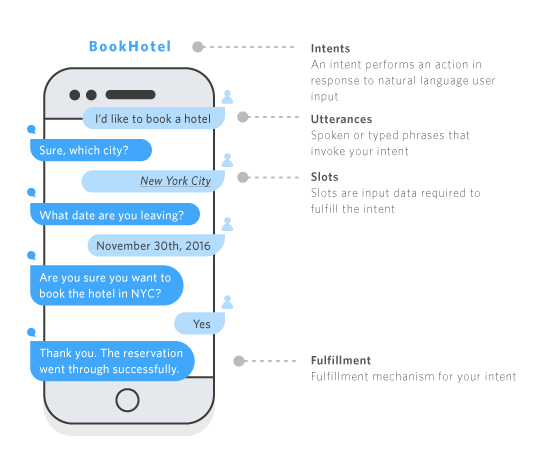
\includegraphics[scale=0.5]{../Immagini/lex_example.png}
	\caption{Utilizzo di Amazon Lex}
\end{figure}

Per quanto riguarda le richieste dell'azienda:
\begin{itemize}
	\item la \textbf{lingua italiana} è supportata;
	\item la \textbf{documentazione} non è chiara, sopratutto per quanto riguarda la creazione di \emph{intent}, \emph{entity} e \emph{utterance};
	\item esiste un piano \textbf{gratuito} per il primo anno di utilizzo di Amazon Lex. Finito, la piattaforma diventa a pagamento in proporzione al numero di chiamate effettuate.
\end{itemize}

\begin{figure}[h]
	\centering
	
\includegraphics[scale=0.6]{../Immagini/amazon-lex.png}
	\caption{Logo di Amazon Lex}
\end{figure}
\newpage
\subsubsection{Api.ai}
Api.ai\footcite{apiai} è uno degli strumenti con il maggior numero di \emph{features} per quanto riguarda il \emph{machine learning} e il \gls{NLP}. Una volta acquistato da Google nel 2016 il suo volume di utilizzatori è aumentato in maniera esponenziale. \\
Api.ai fornisce \gls{SDK} per i principali linguaggi di programmazione tra i quali \emph{C++, C\#, Java, Node.js, JavaScript} e \emph{Python}. Inoltre può essere integrato con \emph{Amazon Echo} e \emph{Microsoft Cortana}. Le applicazioni sviluppate su questa piattaforma sono costituite da \emph{agent}, i quali si occupano di trasformare il linguaggio naturale in dati processabili. Tali \emph{agent} sono a loro volta costituiti da \emph{intent}, che hanno il compito di associare la richiesta dell'utente ad una determinata azione del software, ed \emph{entity}, che sono strumenti per estrarre dal linguaggio naturale i parametri attesi.

Per quanto riguarda le richieste dell'azienda:
\begin{itemize}
	\item la \textbf{lingua italiana} è supportata;
	\item la \textbf{documentazione} è molto chiara;
	\item il suo utilizzo è \textbf{gratuito}, con delle limitazioni per il numero di richieste al minuto, ora, giorno e mese.
\end{itemize}

\begin{figure}[h]
	\centering
	
\includegraphics[scale=0.25]{../Immagini/apiai.png}
	\caption{Logo di api.ai}
\end{figure}

\subsection{Conclusioni dell'analisi}
Dopo una mia attenta analisi sui pregi e difetti di tutti gli strumenti, in accordo con il tutor aziendale, è stata fatta una breve riunione con gli altri dipendenti, dove ho illustrato in modo sintetico i dati raccolti. Amazon Lex e IBM Watson Conversation sono stati considerati non adeguati per lo sviluppo del progetto a causa dei loro costi, mentre le altre piattaforme, non presentando queste limitazioni, potevano essere tutte adottate. \\
La mia proposta è stata quella di utilizzare api.ai, per la maggiore stabilità rispetto a wit.ai, per il maggior numero di lingue disponibili in vista di un supporto futuro ad interazioni con utenti di diversa nazionalità e per la maggiore maturità della piattaforma. L'azienda dopo aver valutato anch'essa i dati raccolti ha deciso di approvare la mia proposta, in quanto api.ai rispettava tutte le sue richieste iniziali, mostrando delle potenzialità molto interessanti per lo sviluppo del prodotto.             % Analisi requisiti
% !TEX encoding = UTF-8
% !TEX TS-program = pdflatex
% !TEX root = ../tesi.tex

%**************************************************************
\chapter{Progettazione}
\label{cap:progettazione}

La progettazione nel caso del prodotto che ho dovuto sviluppare si è concentrata particolarmente sulla piattaforma di api.ai, in quanto rappresentava la maggior parte del lavoro. Successivamente sono passato alla progettazione delle classi da introdurre nel codice già creato dall'azienda, per gestire le nuove funzionalità dei \glspl{chatbot}.

\section{Studio di api.ai}
Prima di passare all'attività di progettazione è stato fondamentale analizzare e studiare a fondo le possibilità che api.ai mette a disposizione per la creazione del prodotto a me richiesto. I concetti base per capire il funzionamento di api.ai sono quattro:
\begin{itemize}
	\item \textbf{agent}: gli \emph{agents} sono meglio descritti come moduli NLU (Natural Language Understanding). Questi possono essere inclusi nell'applicazione, nel prodotto o nel servizio e trasformano le richieste di utenti naturali in dati attivi. Questa trasformazione si verifica quando un input utente corrisponde a uno degli \emph{intent} all'interno dell'\emph{agent};
	\item \textbf{intent}: sono una mappatura tra quello che l'utente può scrivere in input e l'azione che il software deve intraprendere. Un \emph{intent} è formato dalle seguenti sezioni:
	\begin{itemize}
		\item\textbf{ \emph{user says}}: perché l'\emph{agent} capisca la domanda, sono necessari esempi di come la stessa domanda può essere posta in modi diversi. Lo sviluppatore aggiunge queste permutazioni alla sezione \emph{user says} dell'\emph{intent}. Più variazioni vengono aggiunte all'\emph{intent}, meglio l'\emph{agent} comprenderà l'utente;
		\item \textbf{\emph{action}}: contiene il nome della \emph{action}, che può essere utilizzato per attivare una particolare funzione del prodotto, e la tabella dei \textbf{\emph{parameters}}. I \emph{parameters} possono essere intesi come gli elementi che collegano le parole nelle \emph{user says} alle \emph{entities};
		\item \textbf{\emph{response}}: in questa sezione è possibile definire la risposta di api.ai quando l'\emph{intent} viene attivato. Non è stato quasi mai utilizzato, in quanto la risposta viene generata nella \emph{business logic}.
	\end{itemize}
	\item \textbf{context}: i \emph{context} rappresentano il contesto corrente della richiesta di un utente. Ciò è utile per differenziare frasi che possono essere vaghe o avere significati diversi a seconda delle preferenze dell'utente, della posizione geografica, della pagina corrente di un'applicazione o dell'argomento della conversazione. È possibile impostare un \emph{lifespan} ad ognuno di essi per definire dopo quante richieste il \emph{context} deve scadere;
	\item \textbf{entity}: le entities sono strumenti potenti utilizzati per estrarre i valori dei parametri dagli input degli utenti. Tutti i dati importanti che si desidera ottenere dalla richiesta di un utente, avranno un'entità corrispondente. Le \emph{system entities} sono entità pre-costruite fornite da api.ai per facilitare la gestione dei più comuni concetti (luoghi, orari, colori, ecc..). È possibile poi definire le proprie \emph{entities} in base alle necessità dello sviluppatore;
\end{itemize}


\section{Progettazione agents api.ai}
Durante la progettazione degli \emph{agents} per api.ai è stato necessario definire tutti gli \emph{intents} utili a soddisfare i requisiti definiti durante l'analisi dei requisiti. Il passo successivo è stato quello di progettare le \emph{user says} per ogni \emph{intent} e le relative \emph{entity}.

\subsection{Gestore di eventi}
\subsubsection{Intent}
Per quanto riguarda la progettazione del \gls{chatbot} dedicato alla gestione di eventi, gli \emph{intents} che mi sono serviti per soddisfare tutti i requisiti sono stati i seguenti:
\begin{itemize}
	\item \textbf{durata\_conferenza}: permette all'utente di domandare la durata di una conferenza e viene attivato con domande come: \emph{"Quanto dura la conferenza Y?"}. La risposta del \gls{chatbot} contiene il nome, l'inizio, la fine e la durata (in minuti o in ore) della conferenza richiesta dall'ospite;
	\begin{figure}[h]
		\centering
		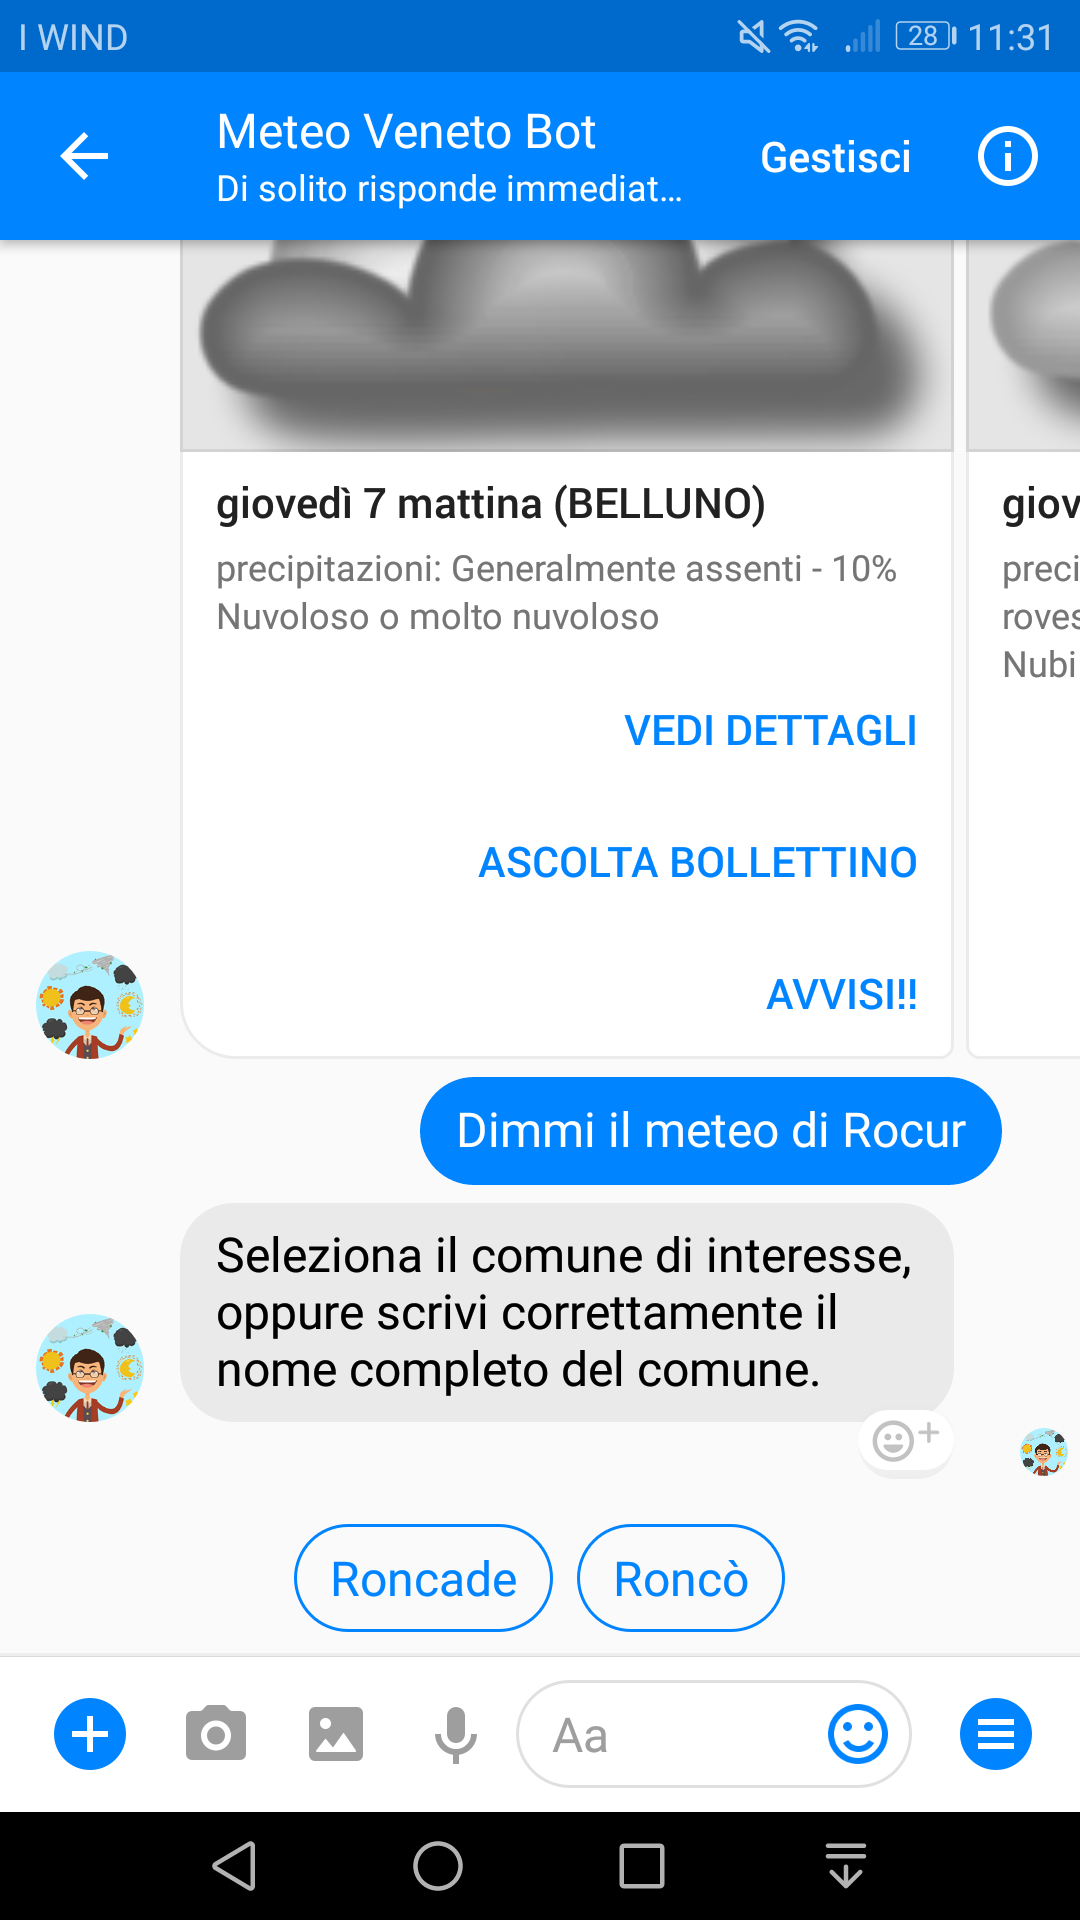
\includegraphics[scale=0.12]{../Immagini/meteo_scelta.png}
		\caption{dfsf}
	\end{figure}
	\item \textbf{luogo\_conferenza}: permette all'utente di domandare il luogo dove si svolgerà la conferenza. La risposta del \gls{chatbot} contiene un carosello predefinito da Messenger, con tutte le informazioni sull'aula in questione;
	\begin{figure}[h!]
		\centering
		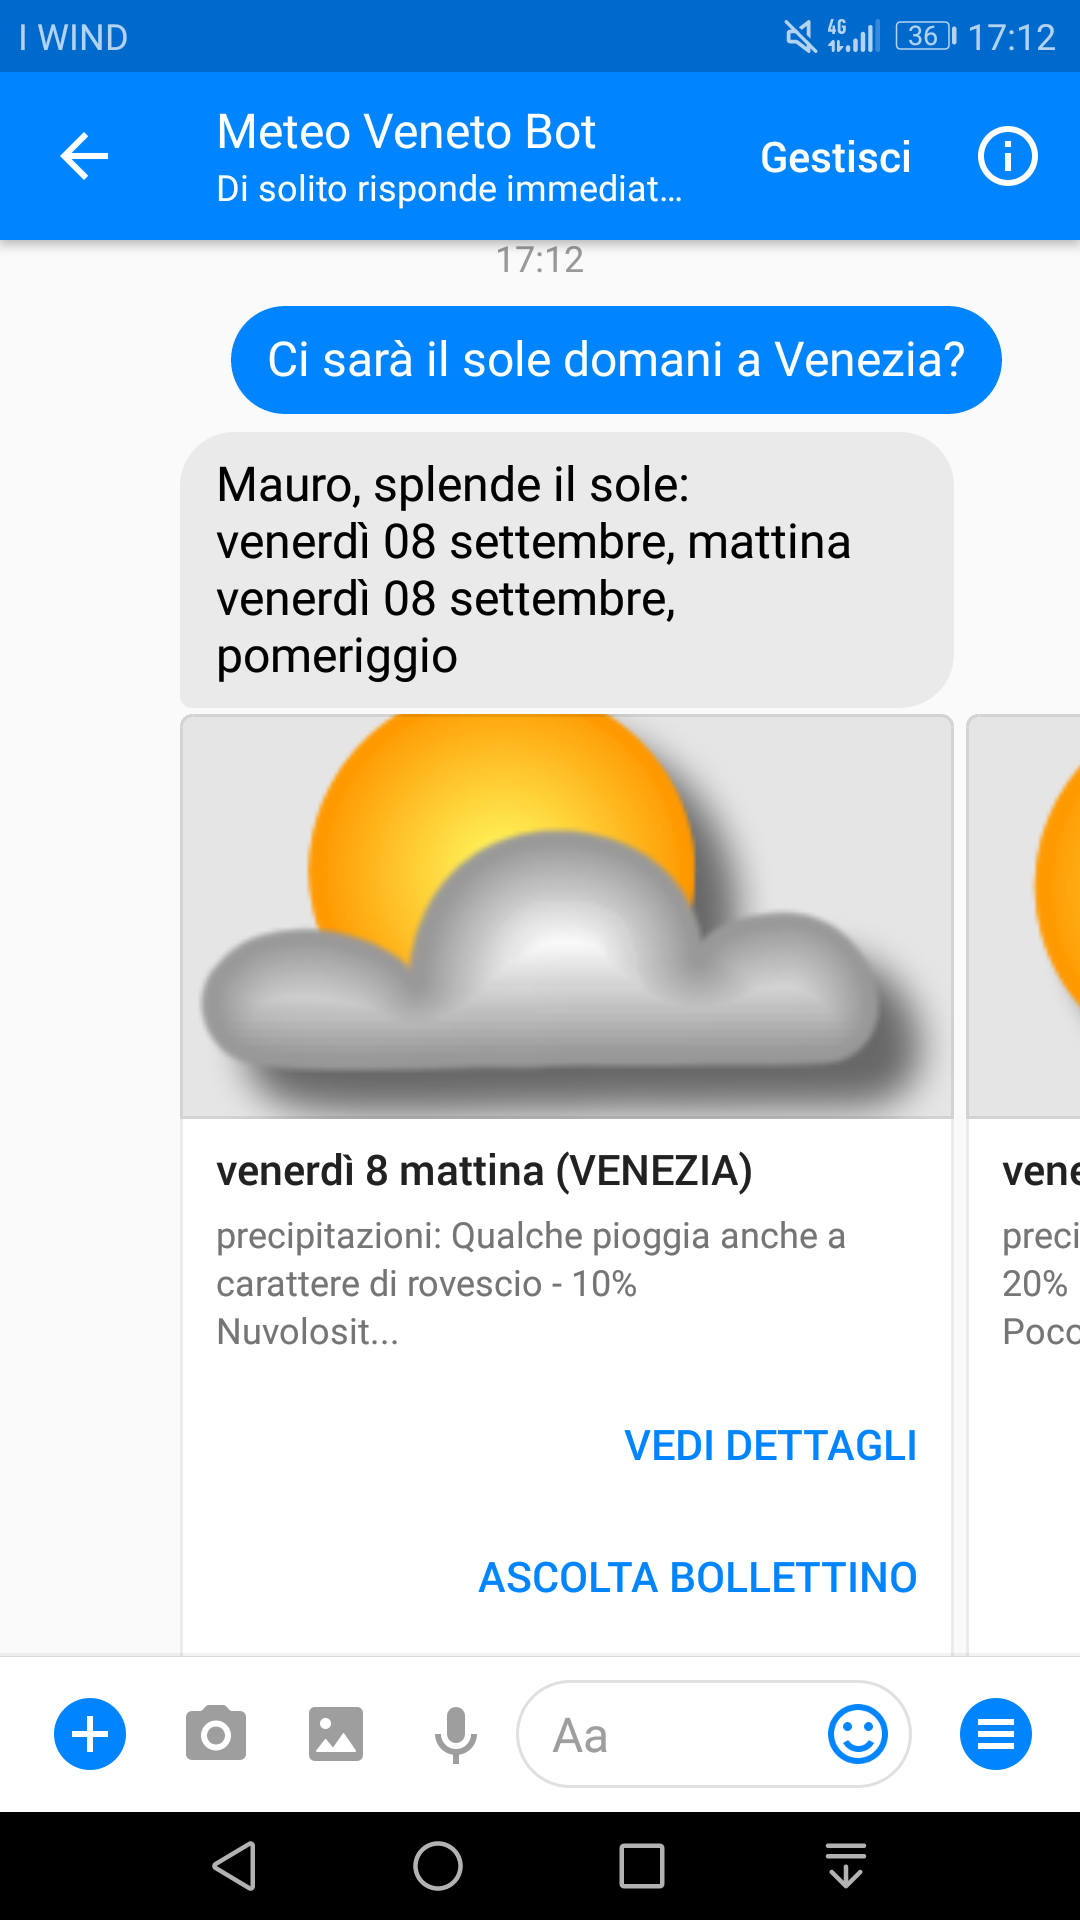
\includegraphics[scale=0.12]{../Immagini/richiesta_sole.png}
		\caption{Esempio di }
	\end{figure}		
	\item \textbf{ora\_conferenza}: permette all'utente di chiedere l'orario di inizio e di fine di una conferenza. La risposta del \gls{chatbot} contiene un carosello predefinito da Messenger, con tutte le informazioni sulla conferenza;
	\begin{figure}[h!]
		\centering
		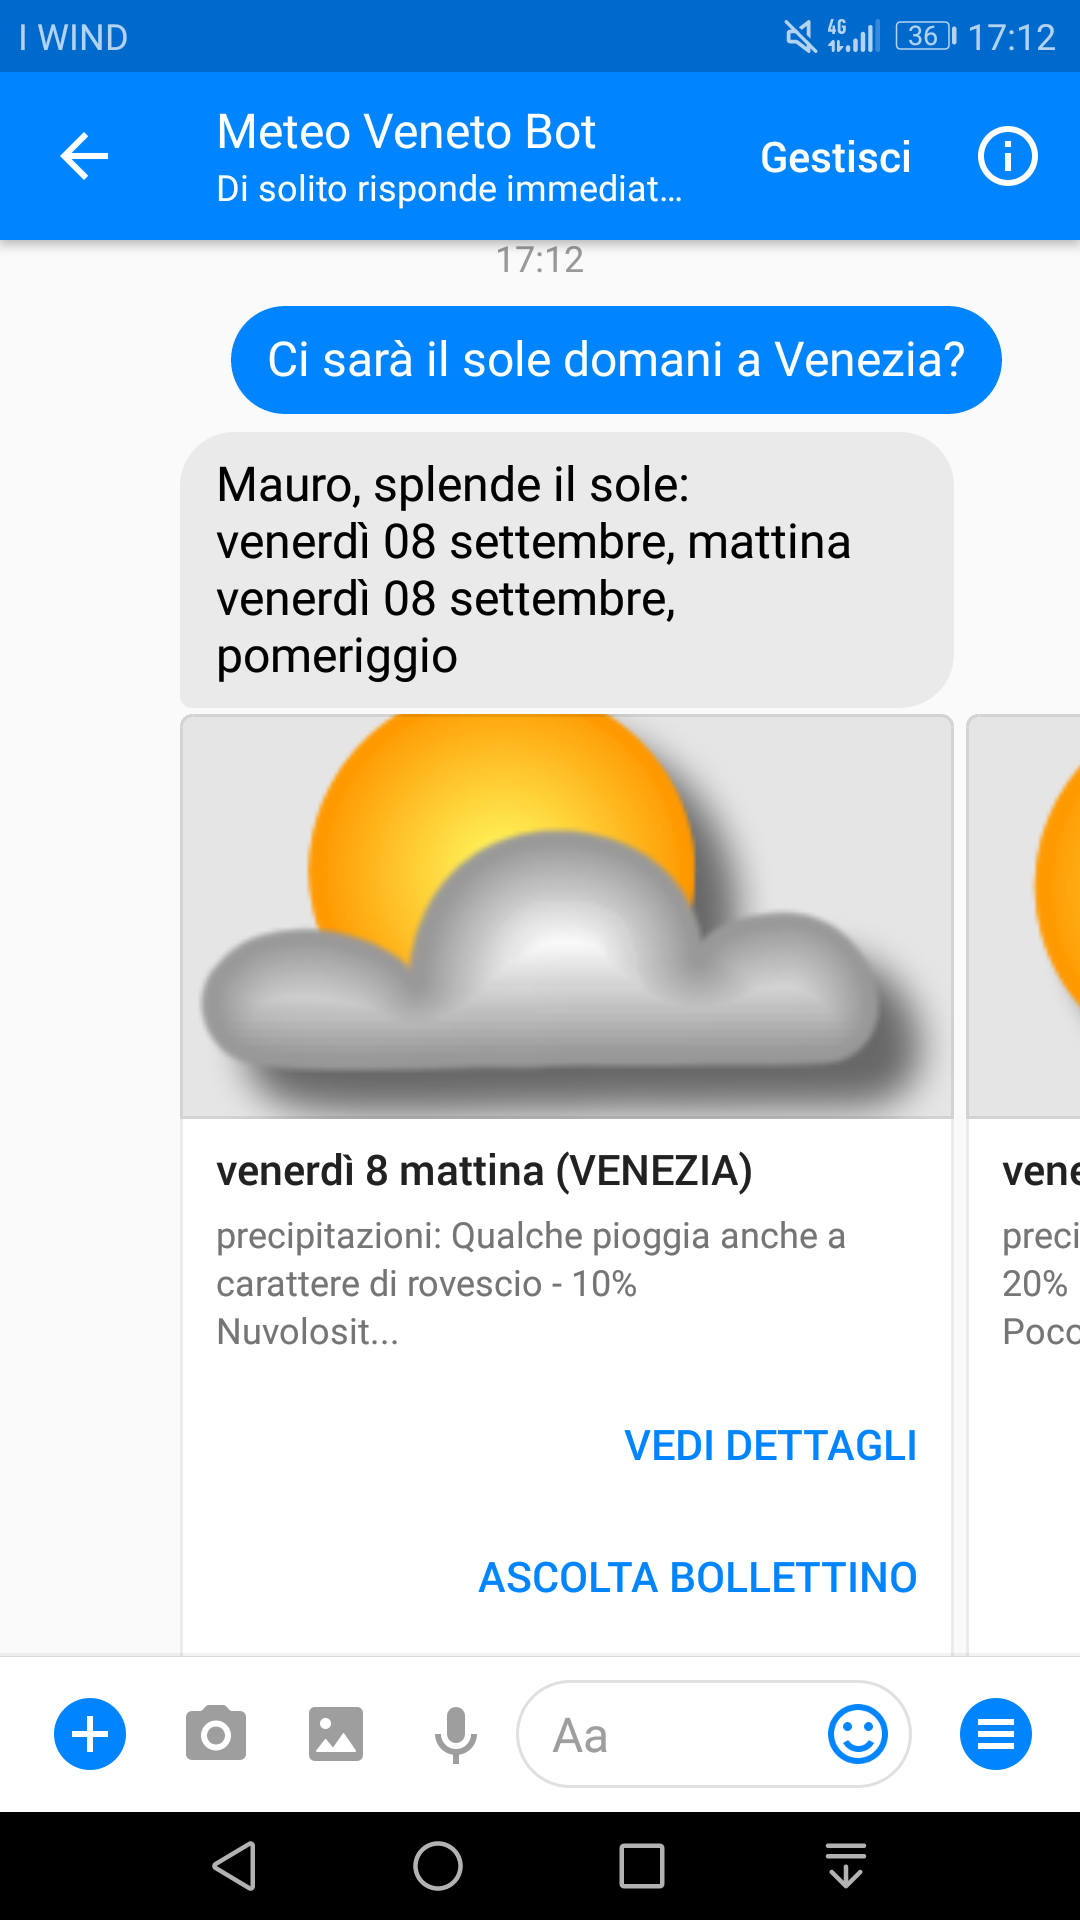
\includegraphics[scale=0.12]{../Immagini/richiesta_sole.png}
		\caption{Esempio di }
	\end{figure}		
	\item \textbf{indicazioni\_stanza}: permette all'utente di domandare le indicazioni per trovare una determinata aula. La risposta del \gls{chatbot} contiene le indicazioni presenti nel database, con una piccola mappa illustrativa;
	\begin{figure}[h!]
		\centering
		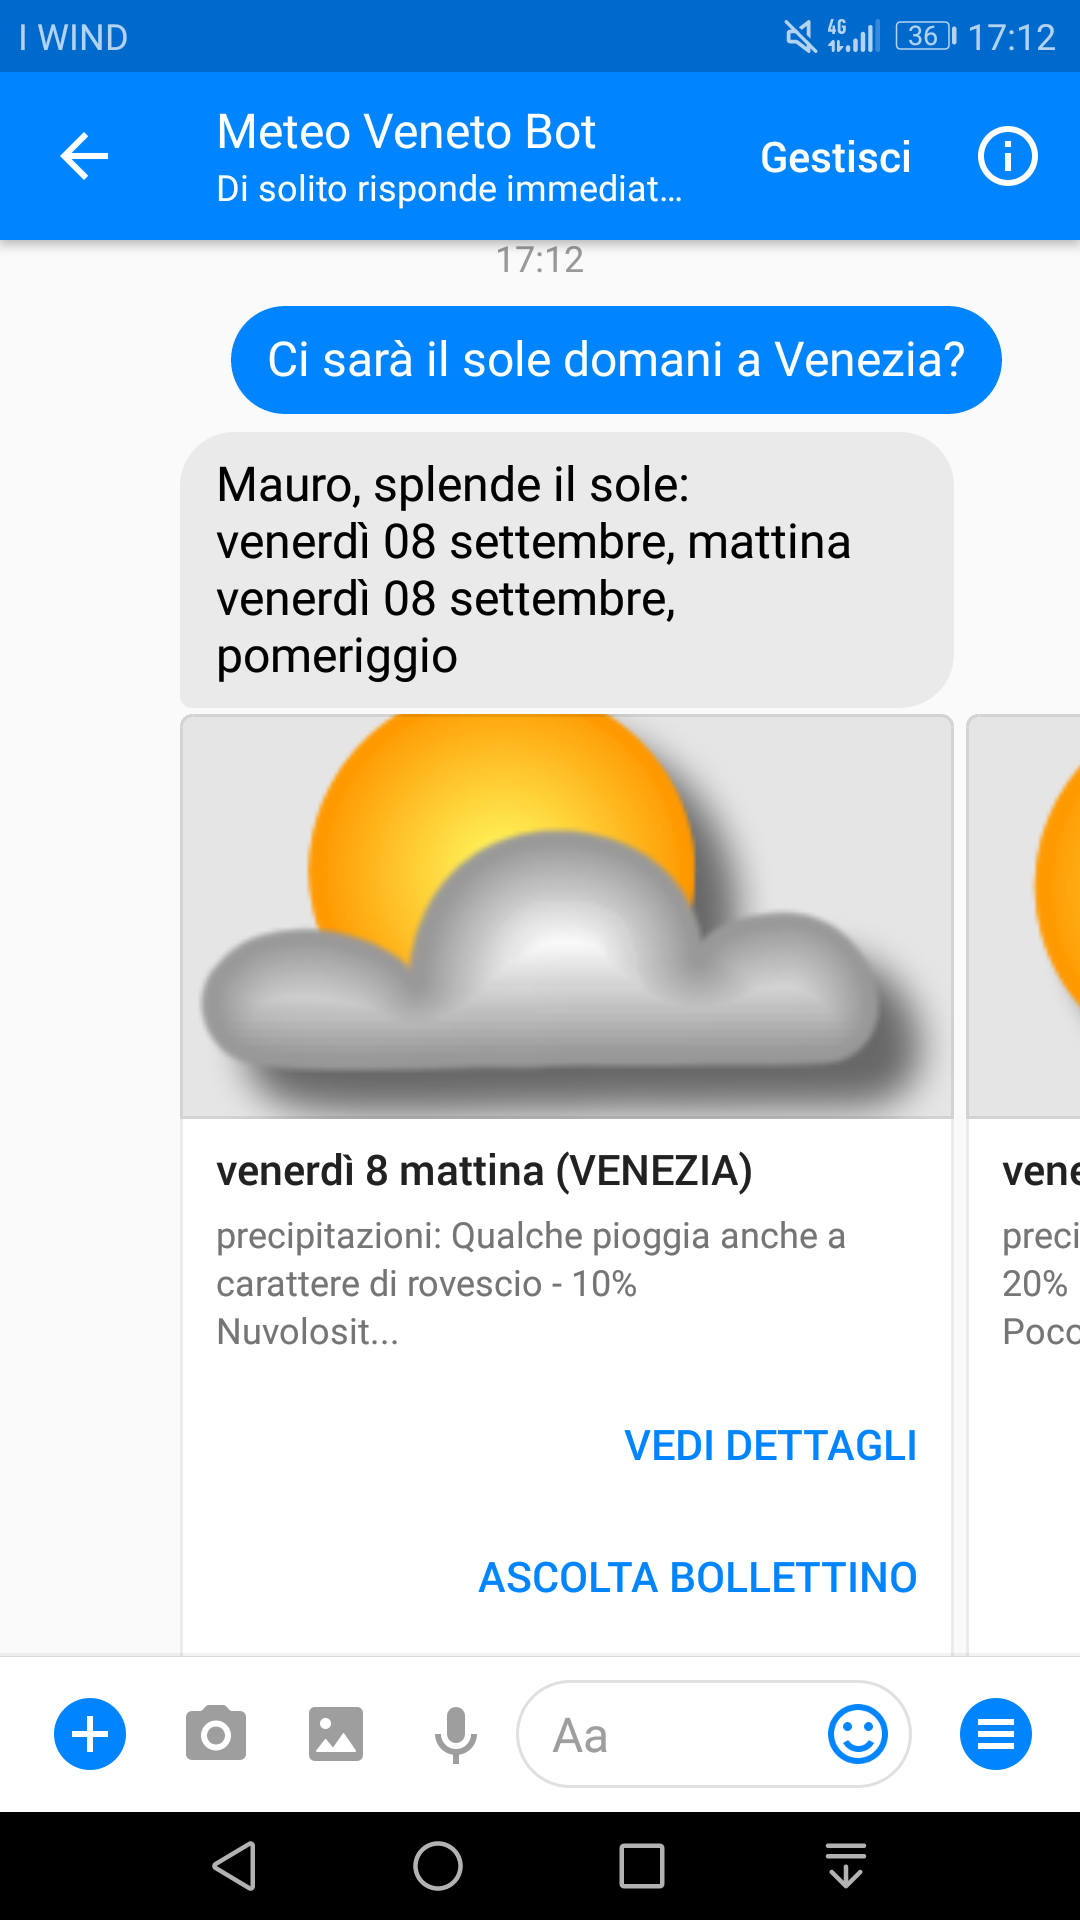
\includegraphics[scale=0.12]{../Immagini/richiesta_sole.png}
		\caption{Esempio di }
	\end{figure}			
	\item \textbf{programma\_giornata}: permette all'utente di domandare il programma dell'evento di un determinato giorno. La risposta del \gls{chatbot} contiene un carosello per ogni conferenza in programma quel giorno;
	\begin{figure}[h!]
		\centering
		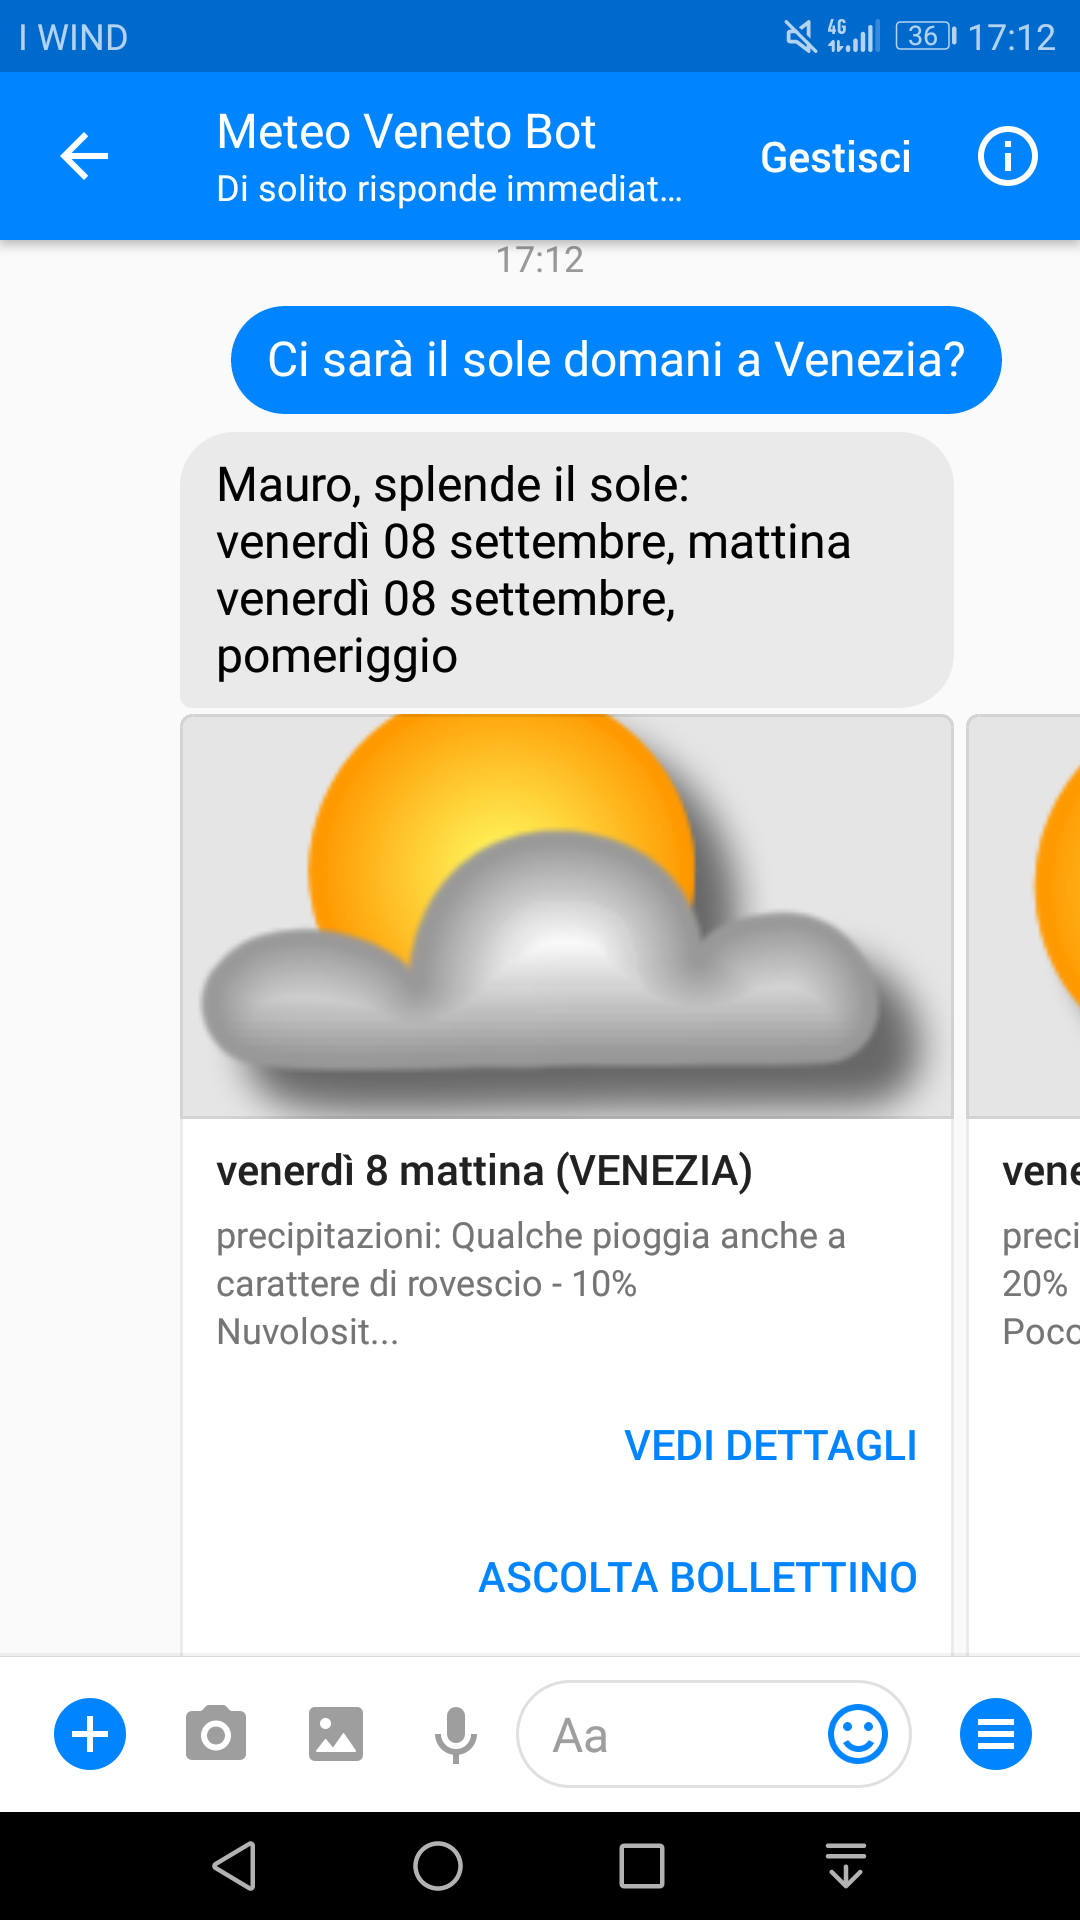
\includegraphics[scale=0.12]{../Immagini/richiesta_sole.png}
		\caption{Esempio di }
	\end{figure}			
	\item \textbf{programma\_no\_data}: permette all'utente di domandare quale conferenza si sta svolgendo in quel momento in una determinata stanza. La risposta del \gls{chatbot} contiene un carosello con la conferenza in programma;
	\begin{figure}[h!]
		\centering
		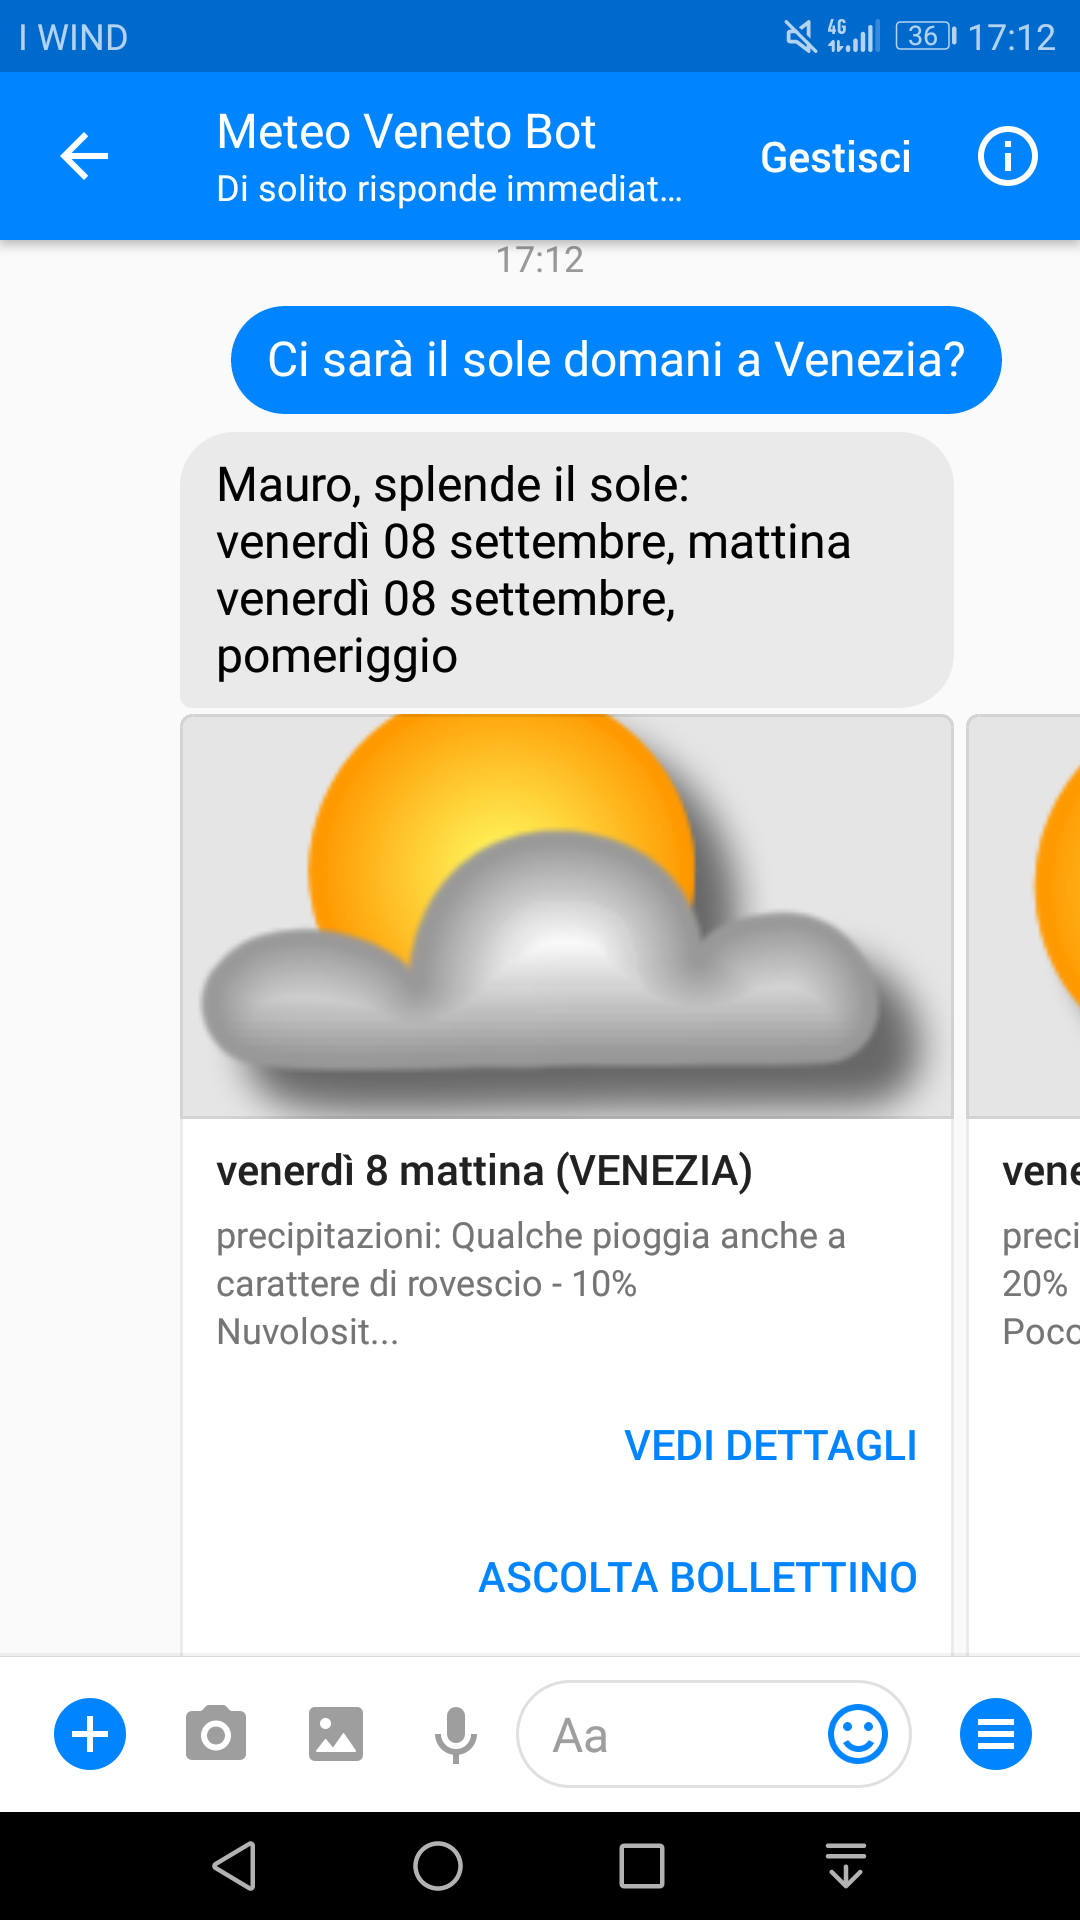
\includegraphics[scale=0.12]{../Immagini/richiesta_sole.png}
		\caption{Esempio di }
	\end{figure}			
	\item \textbf{data\_ora\_stanza\_conferenza}: permette all'utente di domandare la conferenza in programma specificando data, ora e aula. La risposta del \gls{chatbot} contiene un carosello con la conferenza in programma, se presente;
	\begin{figure}[h!]
		\centering
		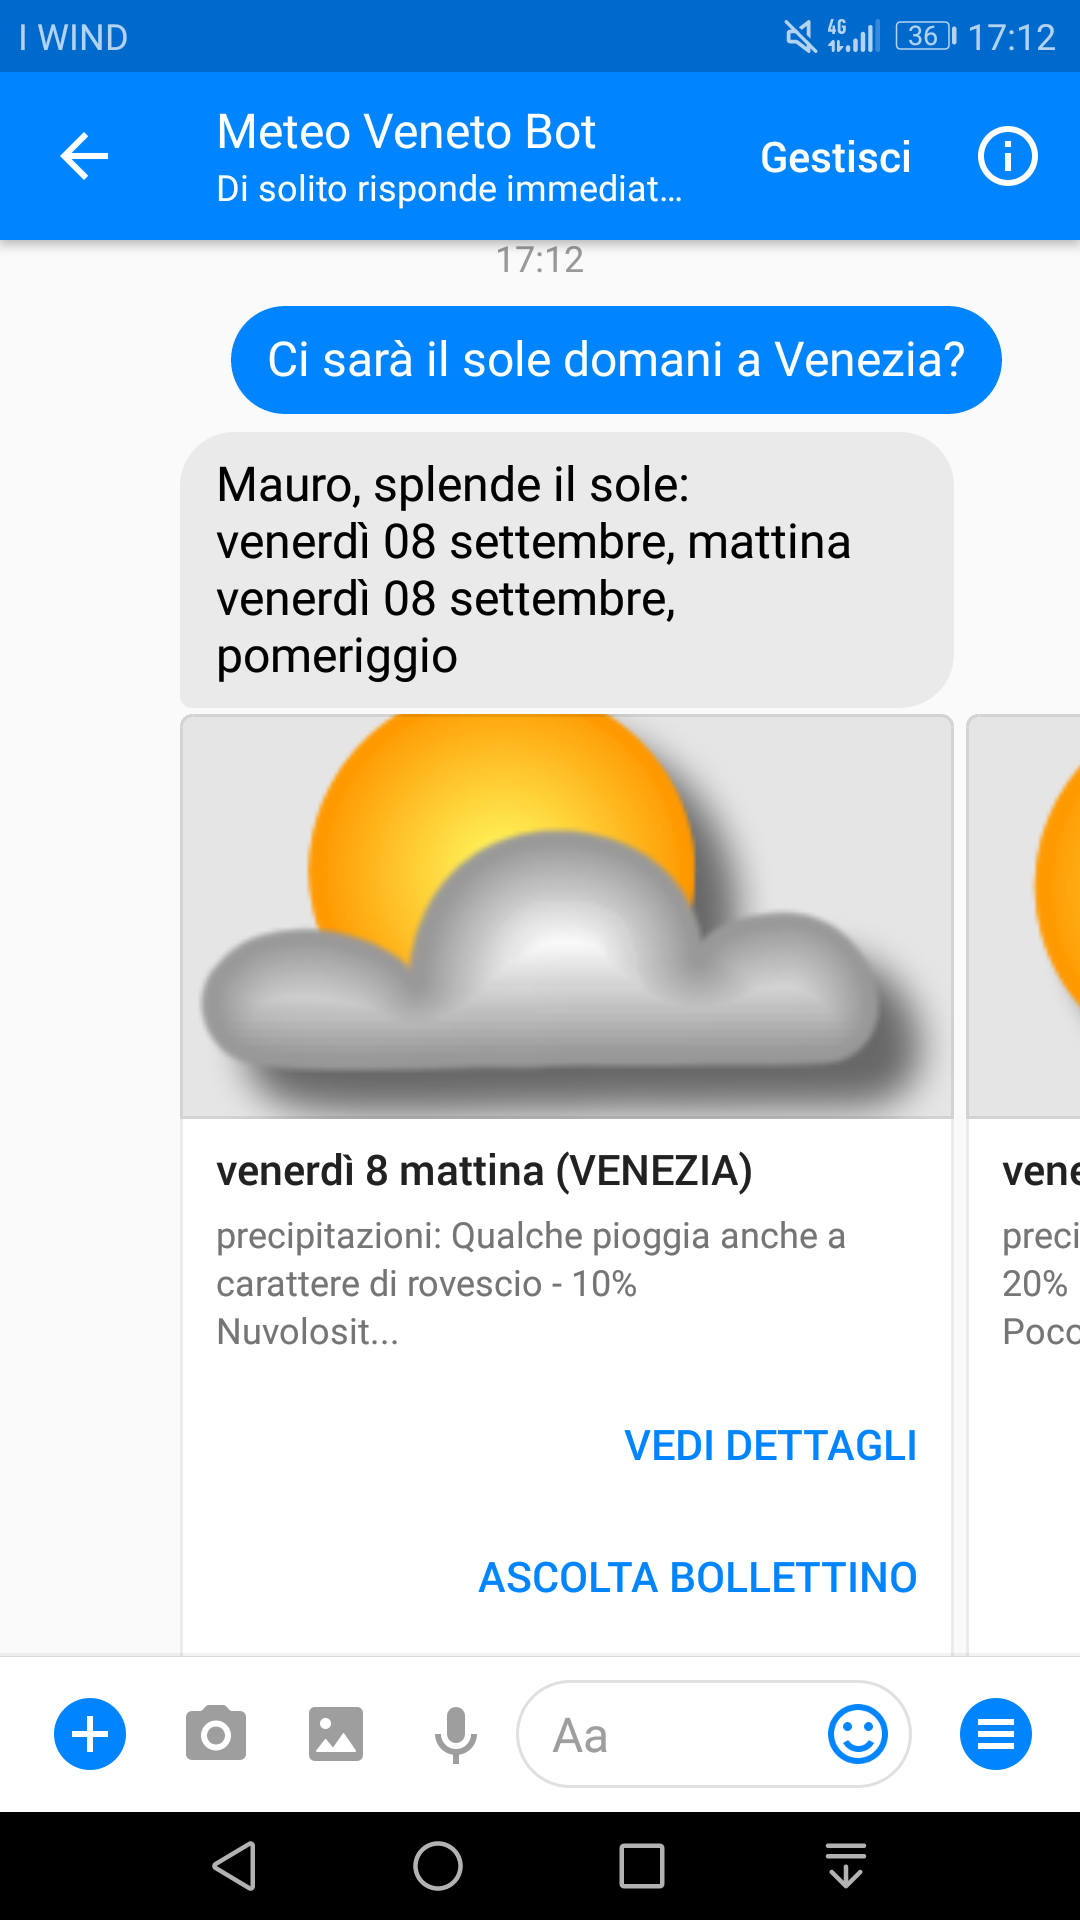
\includegraphics[scale=0.12]{../Immagini/richiesta_sole.png}
		\caption{Esempio di }
	\end{figure}			
	\item \textbf{data\_stanza\_conferenza}: permette all'utente di domandare la conferenza in programma specificando data e aula. La risposta del \gls{chatbot} contiene un carosello con la conferenza in programma, se presente;
	\begin{figure}[h!]
		\centering
		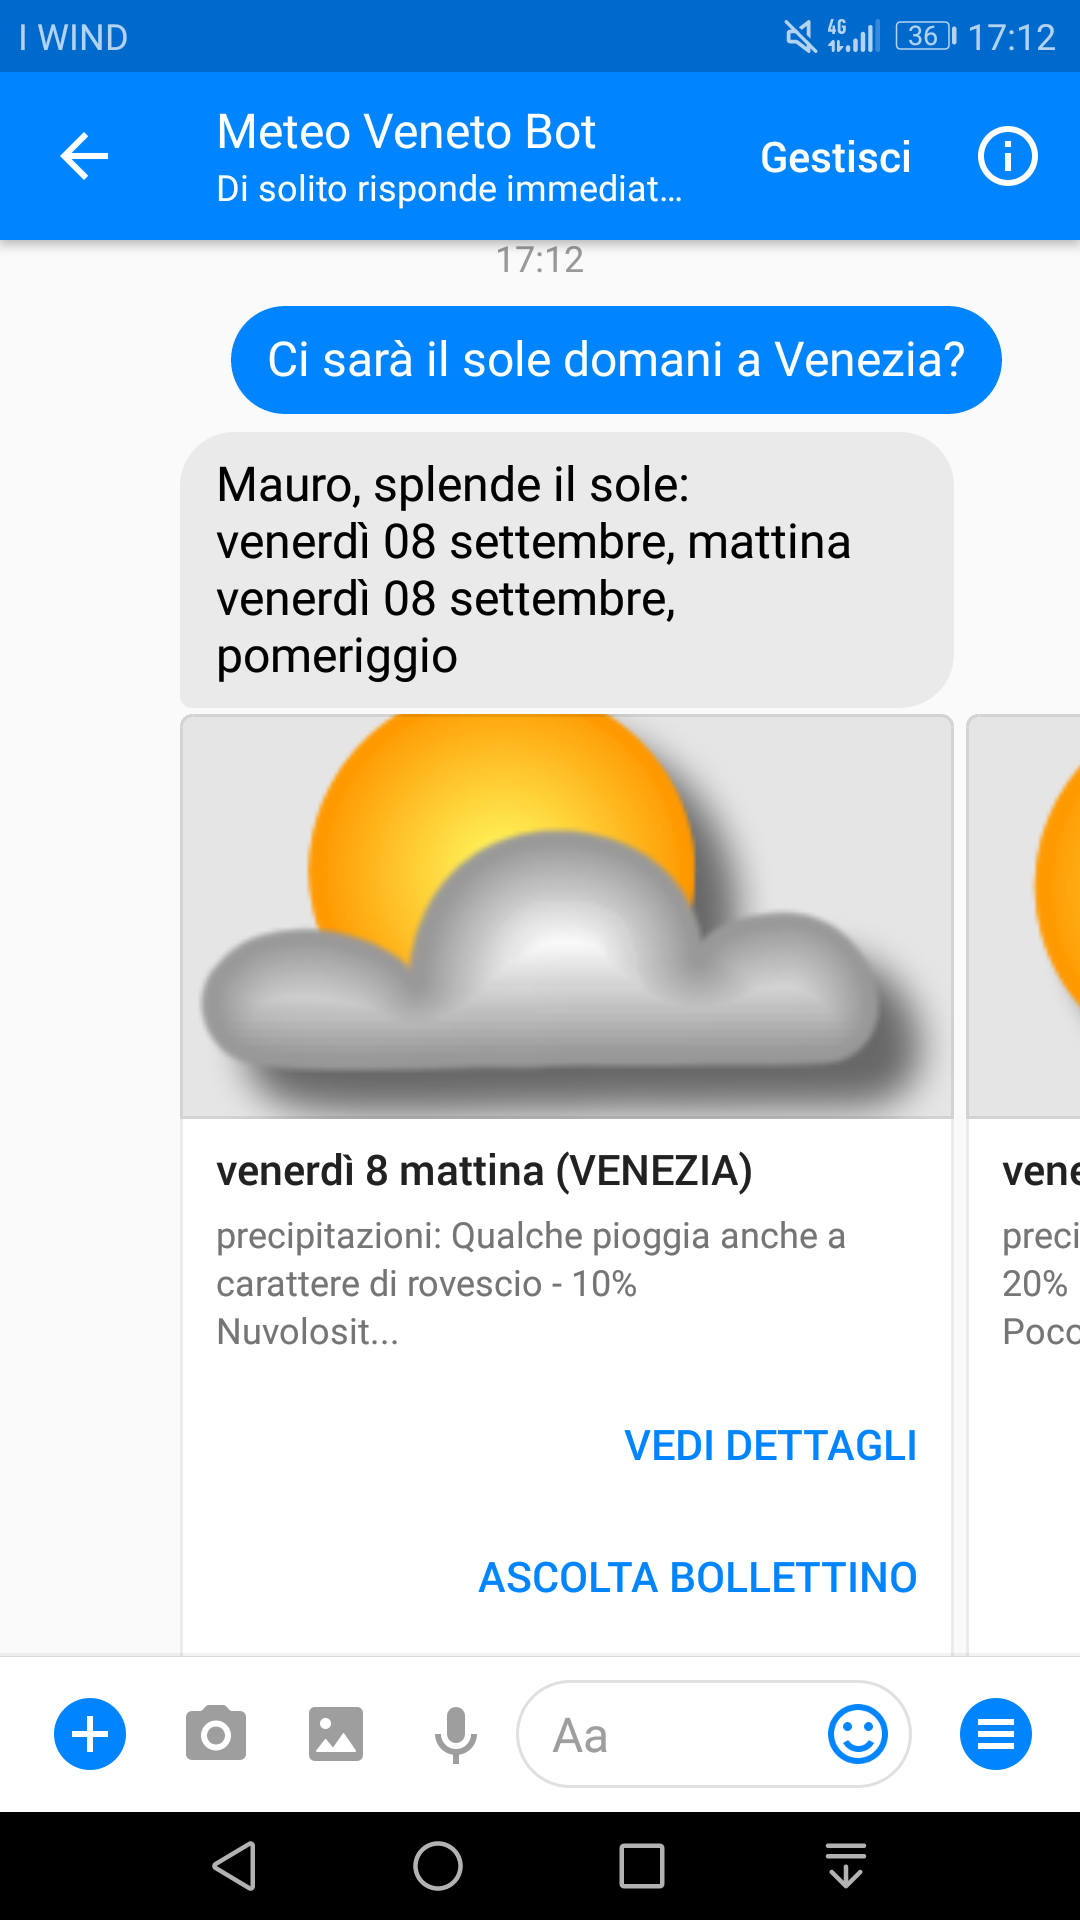
\includegraphics[scale=0.12]{../Immagini/richiesta_sole.png}
		\caption{Esempio di }
	\end{figure}			
	\item \textbf{ora\_stanza\_conferenza}: permette all'utente di domandare la conferenza in programma specificando ora e aula. La risposta del \gls{chatbot} contiene un carosello con la conferenza in programma, se presente;
	\begin{figure}[h!]
		\centering
		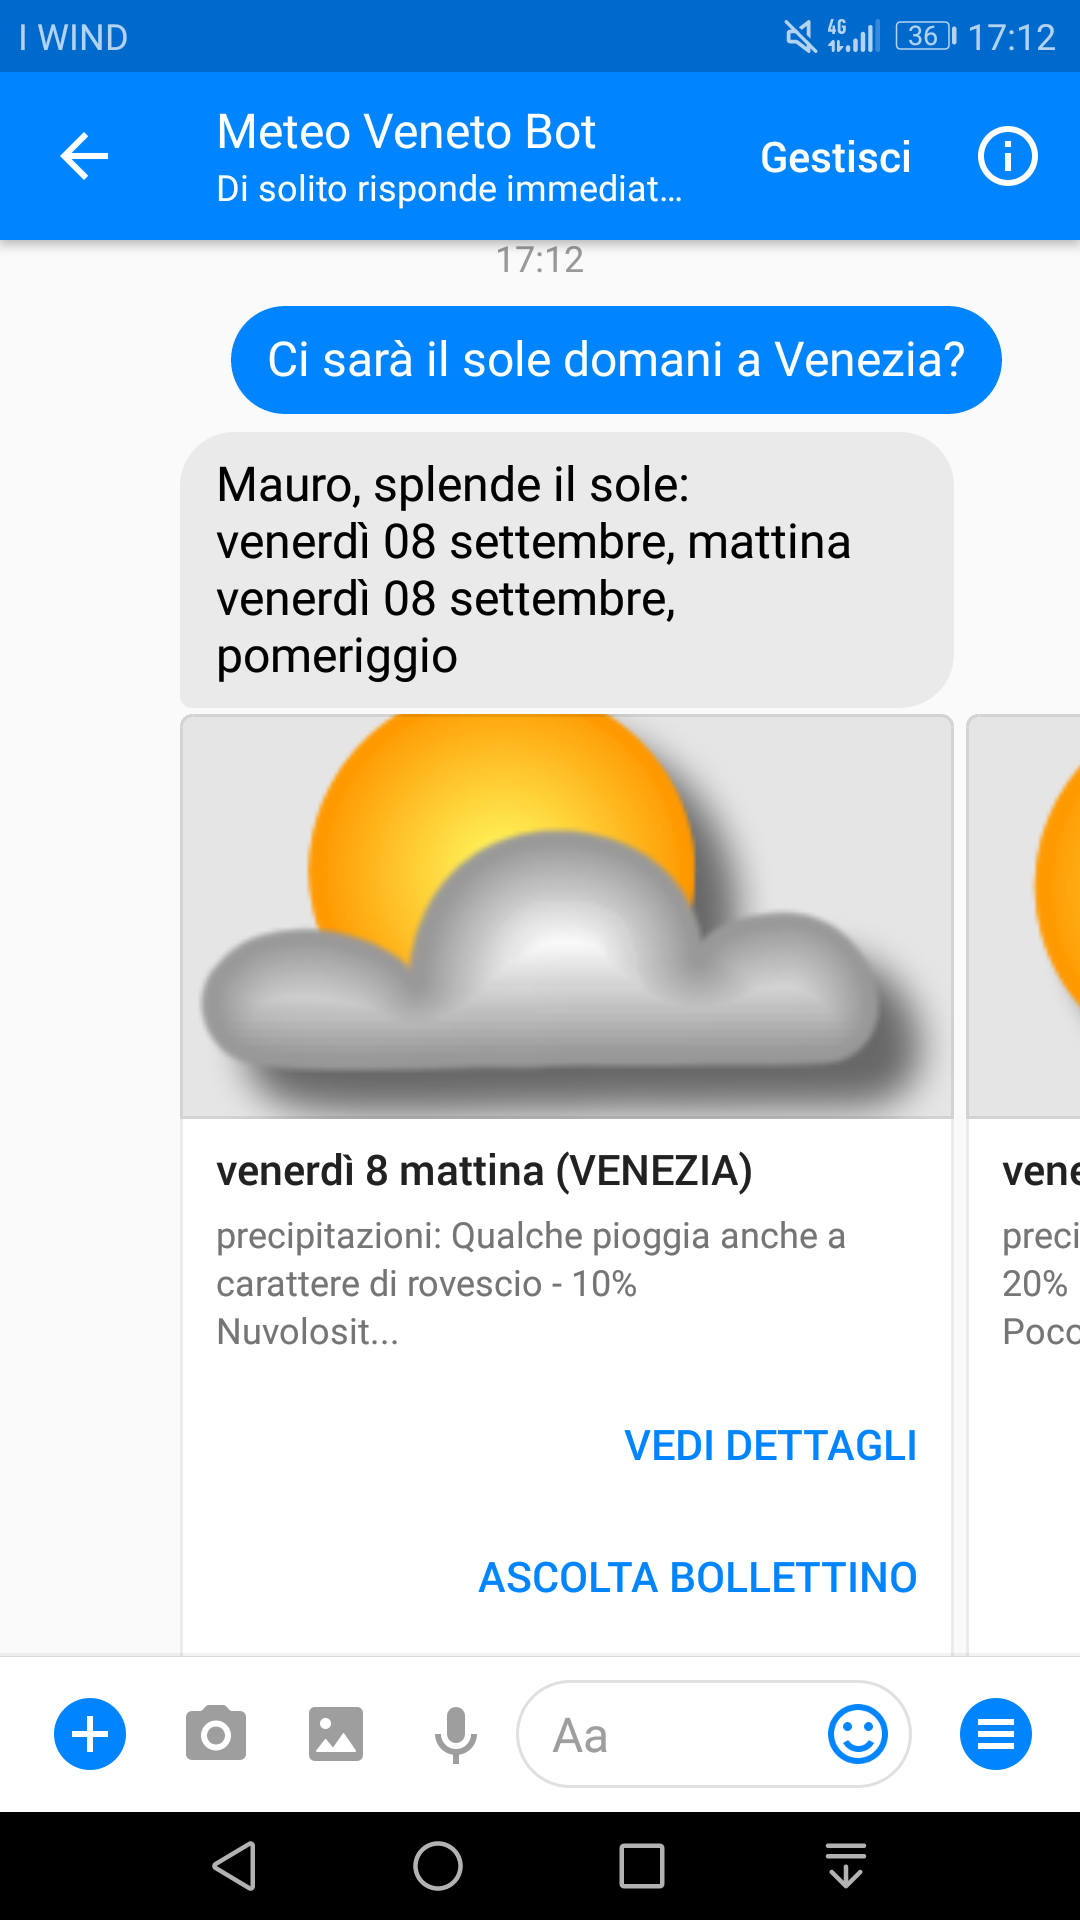
\includegraphics[scale=0.12]{../Immagini/richiesta_sole.png}
		\caption{Esempio di }
	\end{figure}		
	\item \textbf{visualizza\_agenda}: permette all'utente di visualizzare la propria agenda (cioè le conferenze che ha aggiunto precedentemente). La risposta contiene tutte le conferenze aggiunte all'agenda;
	\begin{figure}[h!]
		\centering
		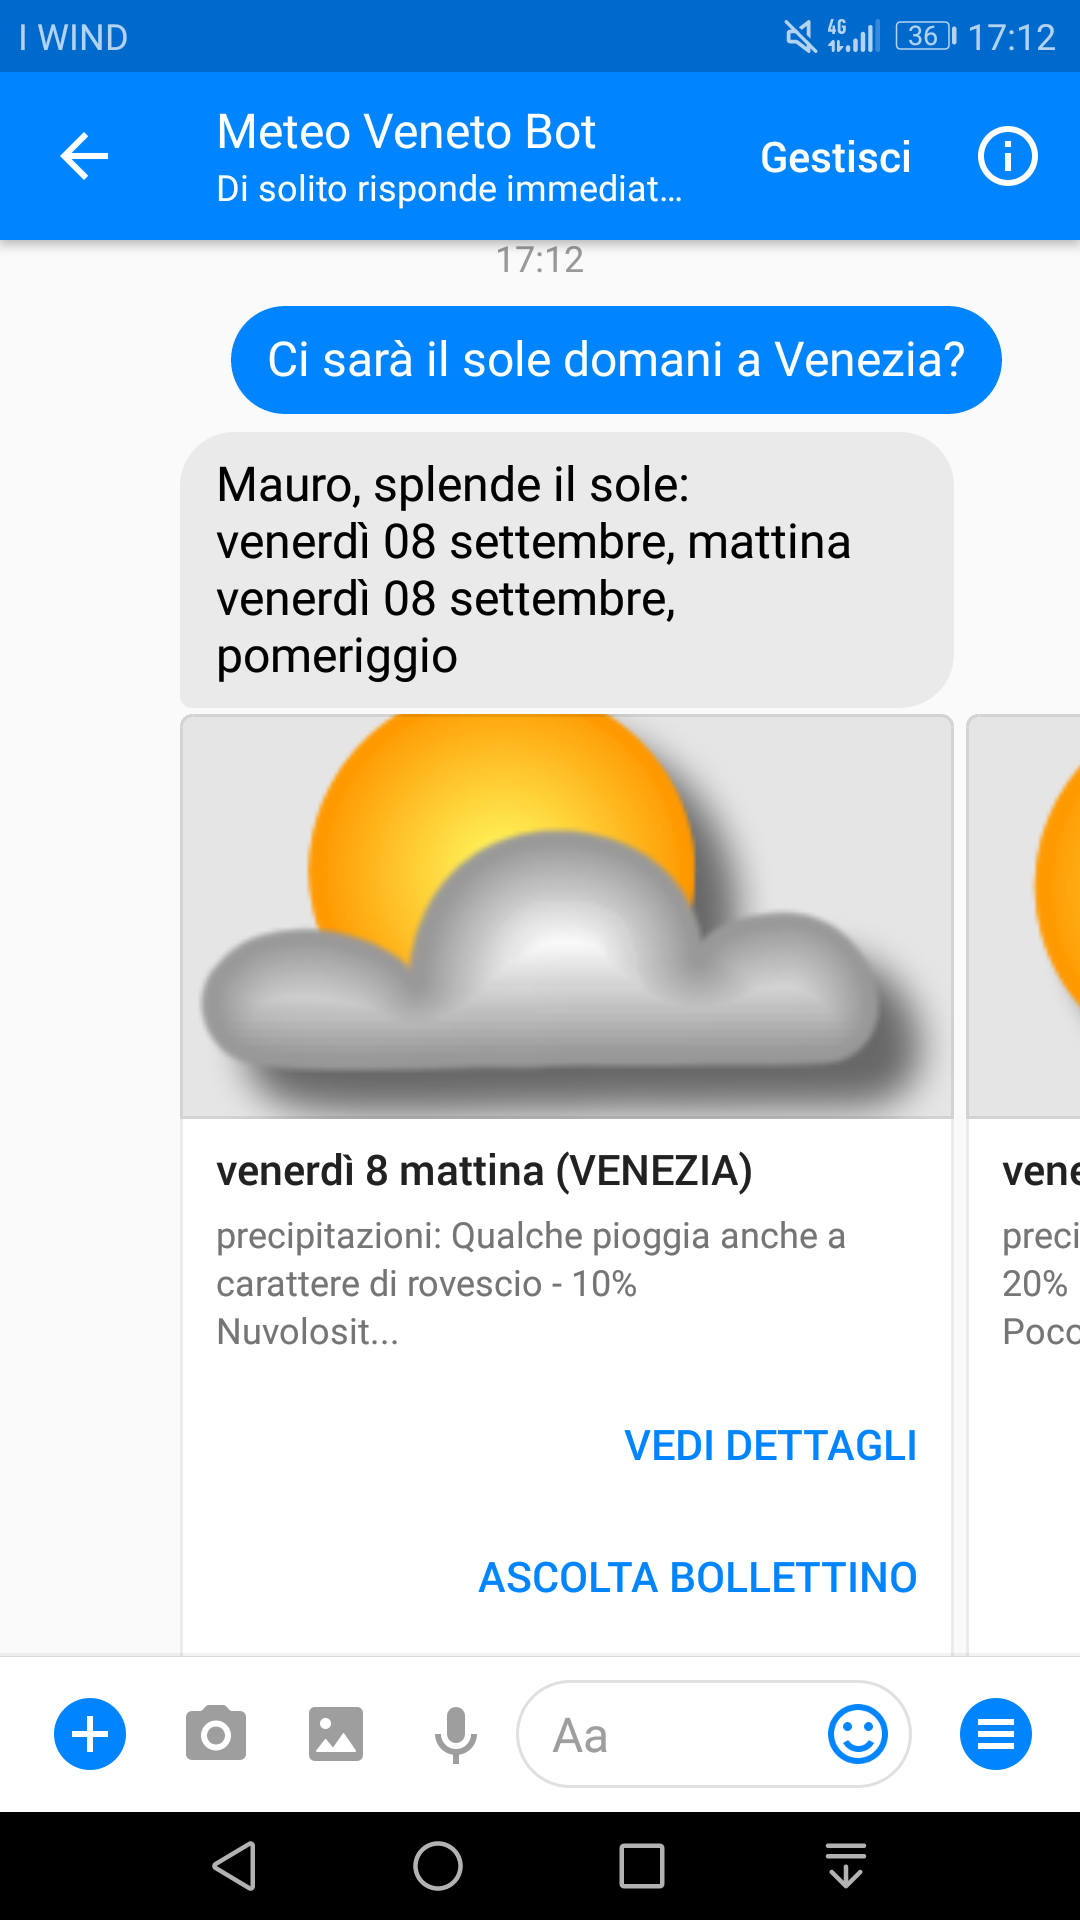
\includegraphics[scale=0.12]{../Immagini/richiesta_sole.png}
		\caption{Esempio di }
	\end{figure}			
	\item \textbf{richiesta\_aiuto}: permette all'utente di ottenere delle informazioni per l'utilizzo del \gls{chatbot}. La risposta contiene una breve spiegazione e delle domande che possono essere rivolte al bot.
\end{itemize}
\newpage
\subsubsection{Entity}
Nella progettazione di questo \emph{agent} ho creato queste nuove \emph{entities}:
\begin{itemize}
	\item \textbf{conference}: viene utilizzata per gestire i sinonimi della parola "conferenza". In questo modo scrivere assemblea, meeting ha lo stesso risultato di conferenza;
	\item \textbf{stanza}: viene utilizzata per gestire i sinonimi della parola "stanza". In questo modo l'utente può scrivere aula, sala, padiglione con lo stesso risultato di stanza;
	\item \textbf{my\_time}: questa \emph{entity} è formata da \emph{@sys.time}, ossia una \emph{system entity} fornita da api.ai per estrarre un orario dall'input dell'utente, e una serie di espressioni per indicare il momento attuale in cui l'utente fa la domanda (adesso, in questo momento, ora). In questo modo se l'utente scrive \emph{"Cosa fanno in aula X adesso?"}, nel \gls{JSON} ritornato da api.ai ci sarà un parametro di tipo \emph{my\_time} con valore "adesso", che potrà essere gestito nella \emph{business logic}.
\end{itemize}

\begin{figure}[h!]
	\centering
	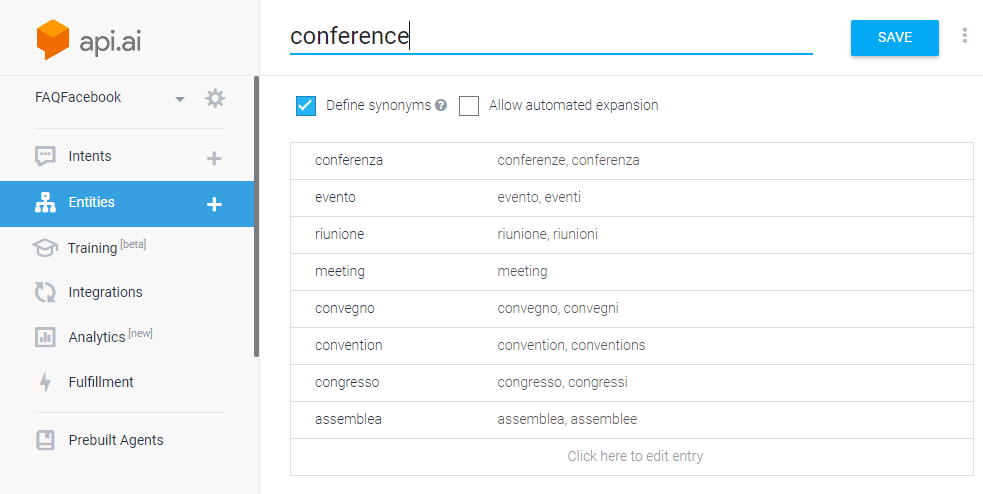
\includegraphics[scale=0.5]{../Immagini/conference.png}
	\caption{Entity conference definita nell'agent}
\end{figure}

\subsection{Dati ARPA Veneto}
Il \gls{chatbot} dedicato al meteo è stato realizzato grazie agli \emph{open data} messi a disposizione dall'Agenzia Regionale per la Prevenzione e Protezione Ambientale del Veneto(ARPAV). Ogni giorno, nel sito ufficiale\footcite{arpav}, vengono emessi tre bollettini:
\begin{itemize}
	\item \textbf{alle 9:00}: che rappresenta un aggiornamento del bollettino del giorno precedente;
	\item \textbf{alle 13:00}: il nuovo bollettino;
	\item \textbf{alle 16:00}: un aggiornamento del bollettino emesso alle 13.
\end{itemize} 

Il file \gls{XML} che è possibile scaricare, contiene queste informazioni:
\begin{itemize}
	\item le previsioni dei cinque giorni successivi per le 18 zone in cui è stata divisa la regione del Veneto;
	\item una descrizione dell'evoluzione generale dei cinque giorni successivi, per tre macro zone: la regione intera, la zona delle Dolomiti e la pianura veneta.
\end{itemize}

Ad ogni nuova emissione del bollettino, i nuovi dati vengono inseriti nel database aziendale, in modo da comunicare agli utenti solamente le notizie più aggiornate.

\subsection{Meteo Veneto Bot}
\subsubsection{Intent}
Gli intents che ho deciso di creare per soddisfare tutti i requisiti sono i seguenti:
\begin{itemize}
	\item \textbf{richiesta\_meteo}: permette all'utente di chiedere le previsioni del meteo specificando una giornata o un periodo di tempo (es. weekend) e il comune di interesse (se non viene specificato, si considera il comune da lui selezionato all'inizio dell'interazione con il \gls{chatbot}). La risposta contiene un carosello con il meteo richiesto.
	\begin{figure}[h]
		\centering
		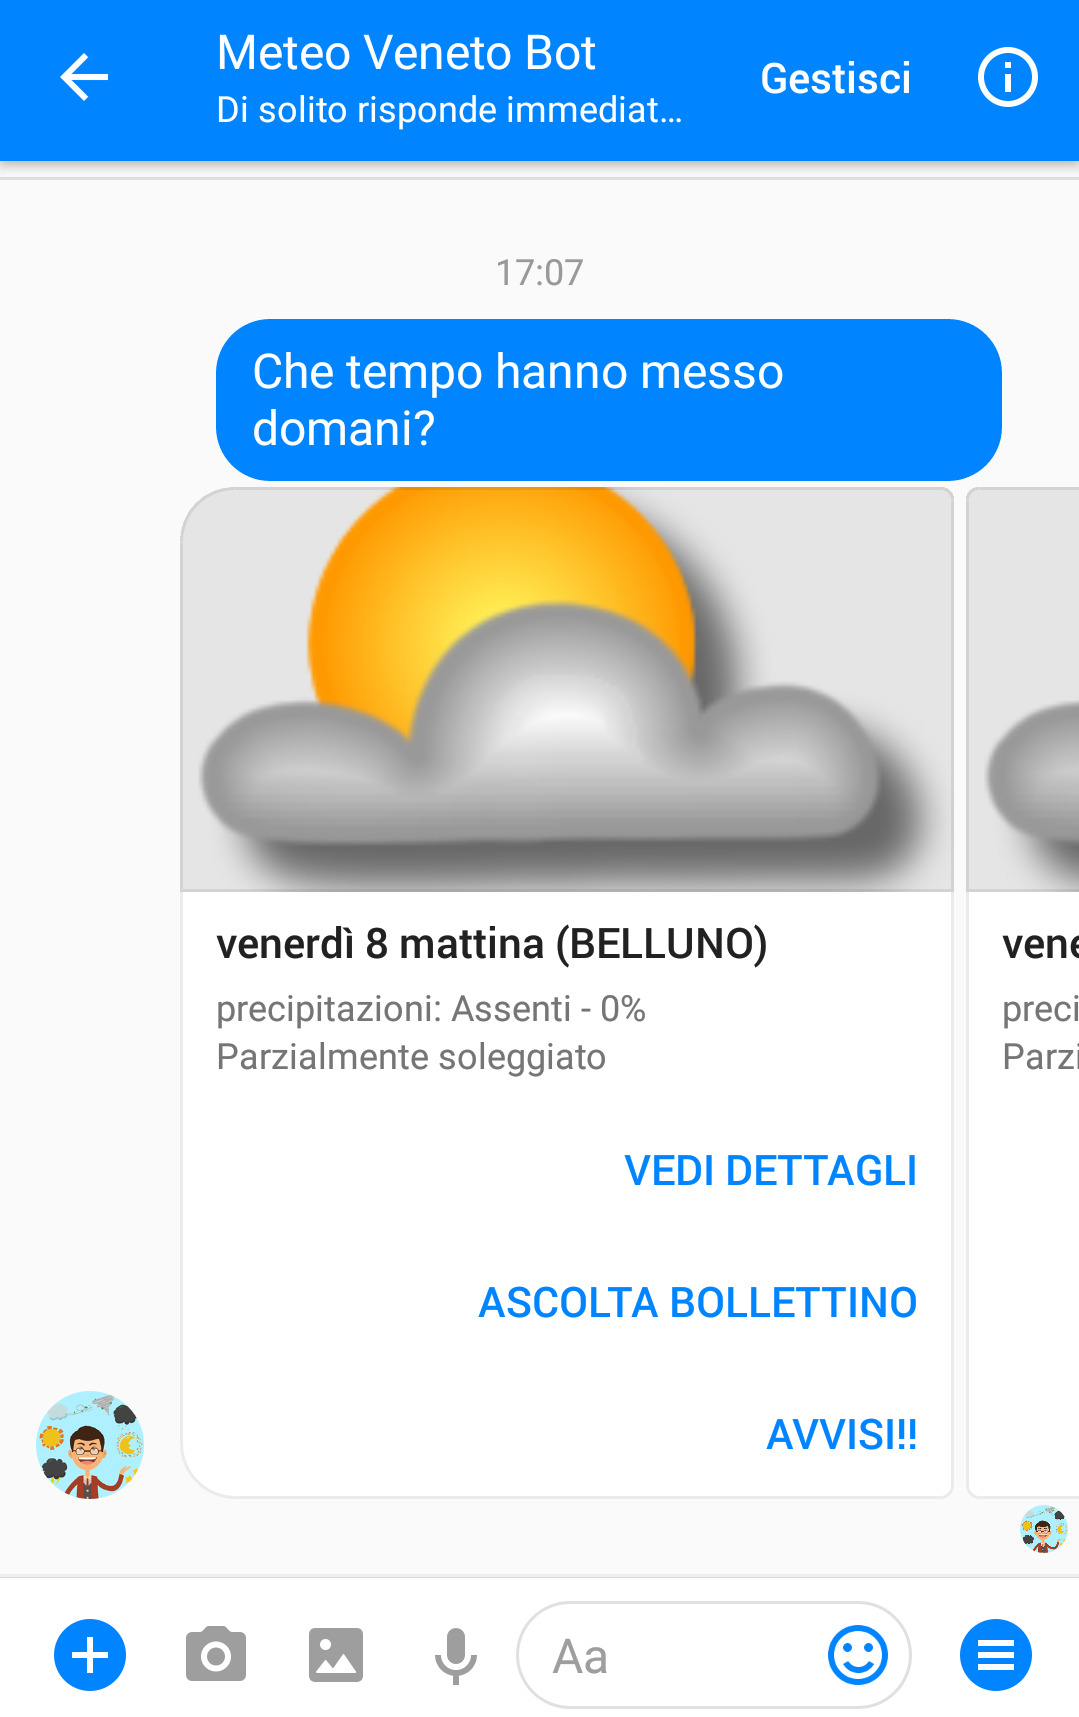
\includegraphics[scale=0.12]{../Immagini/richiesta_meteo.png}
		\caption{Esempio di }
	\end{figure}	
	\item \textbf{richiesta\_sole}: permette all'utente di chiedere se è previsto il sole in una specifica giornata o un periodo di tempo (es. weekend), in un determinato comune. La risposta è formata da due messaggi: il primo mostra le giornate dove è previsto il sole, tra quelle richieste dall'utente, il secondo contiene i caroselli delle previsioni.
	\begin{figure}[!h]
		\centering
		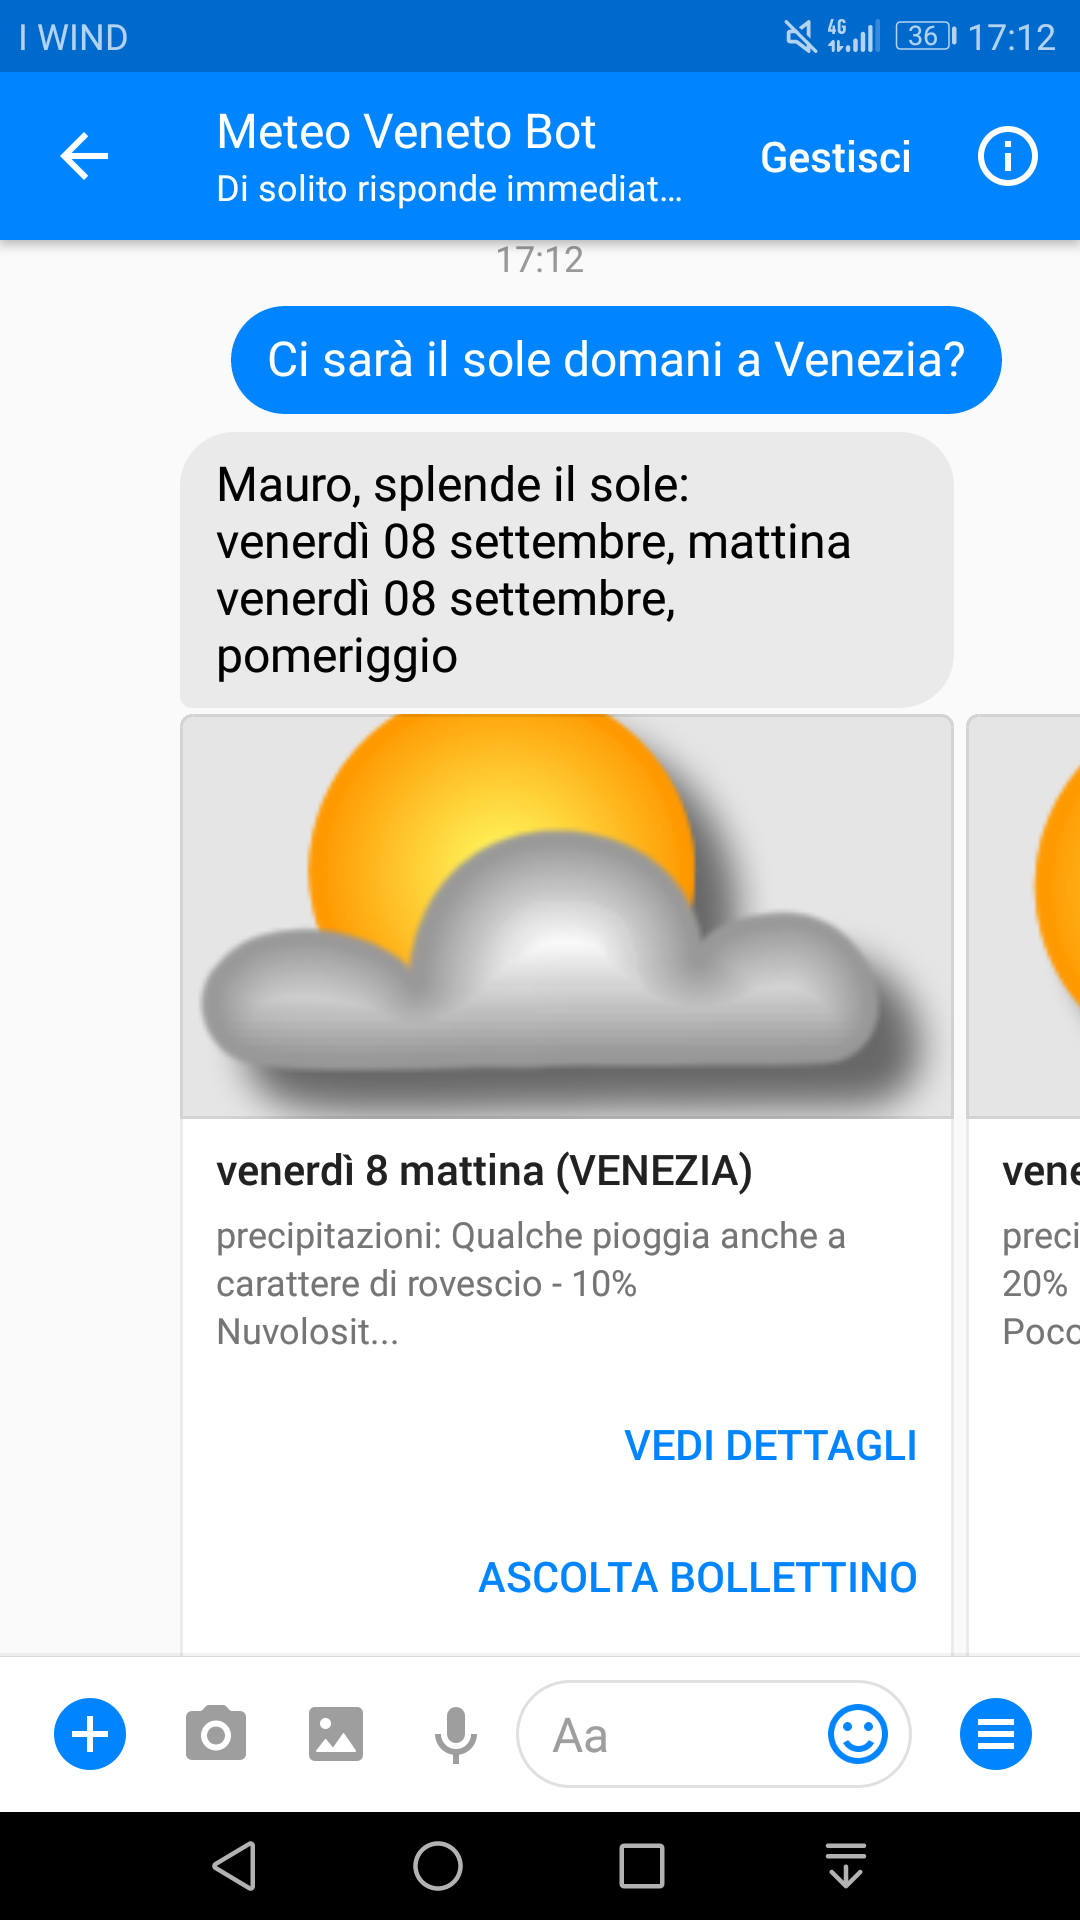
\includegraphics[scale=0.12]{../Immagini/richiesta_sole.png}
		\caption{Esempio di }
	\end{figure}	
	\item \textbf{richiesta\_pioggia}: permette all'utente di chiedere se è prevista pioggia in una specifica giornata o un periodo di tempo (es. weekend), in un determinato comune. La risposta è formata da due messaggi: il primo mostra le giornate dove è prevista pioggia, tra quelle richieste dall'utente, il secondo contiene i caroselli delle previsioni.
	\begin{figure}[!h]
		\centering
		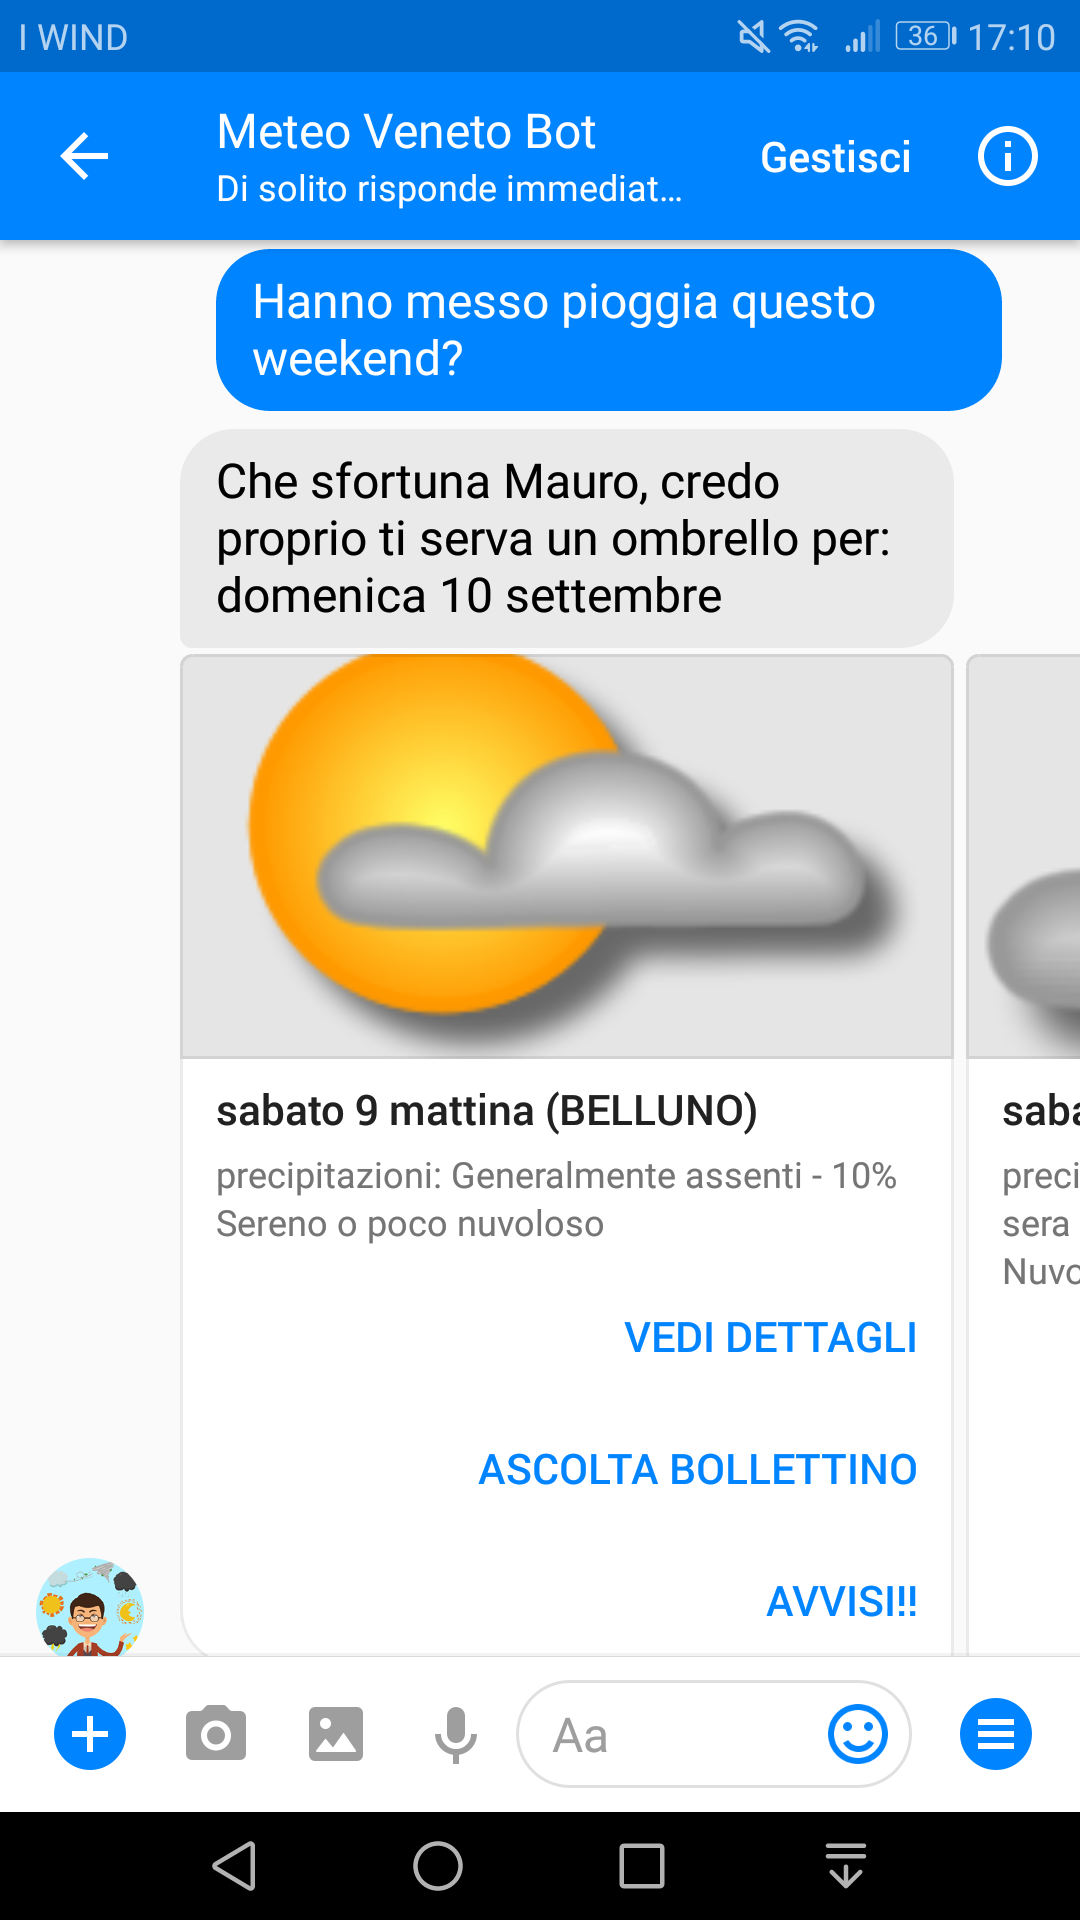
\includegraphics[scale=0.12]{../Immagini/richiesta_pioggia.png}% "%" necessario
		\qquad\qquad
		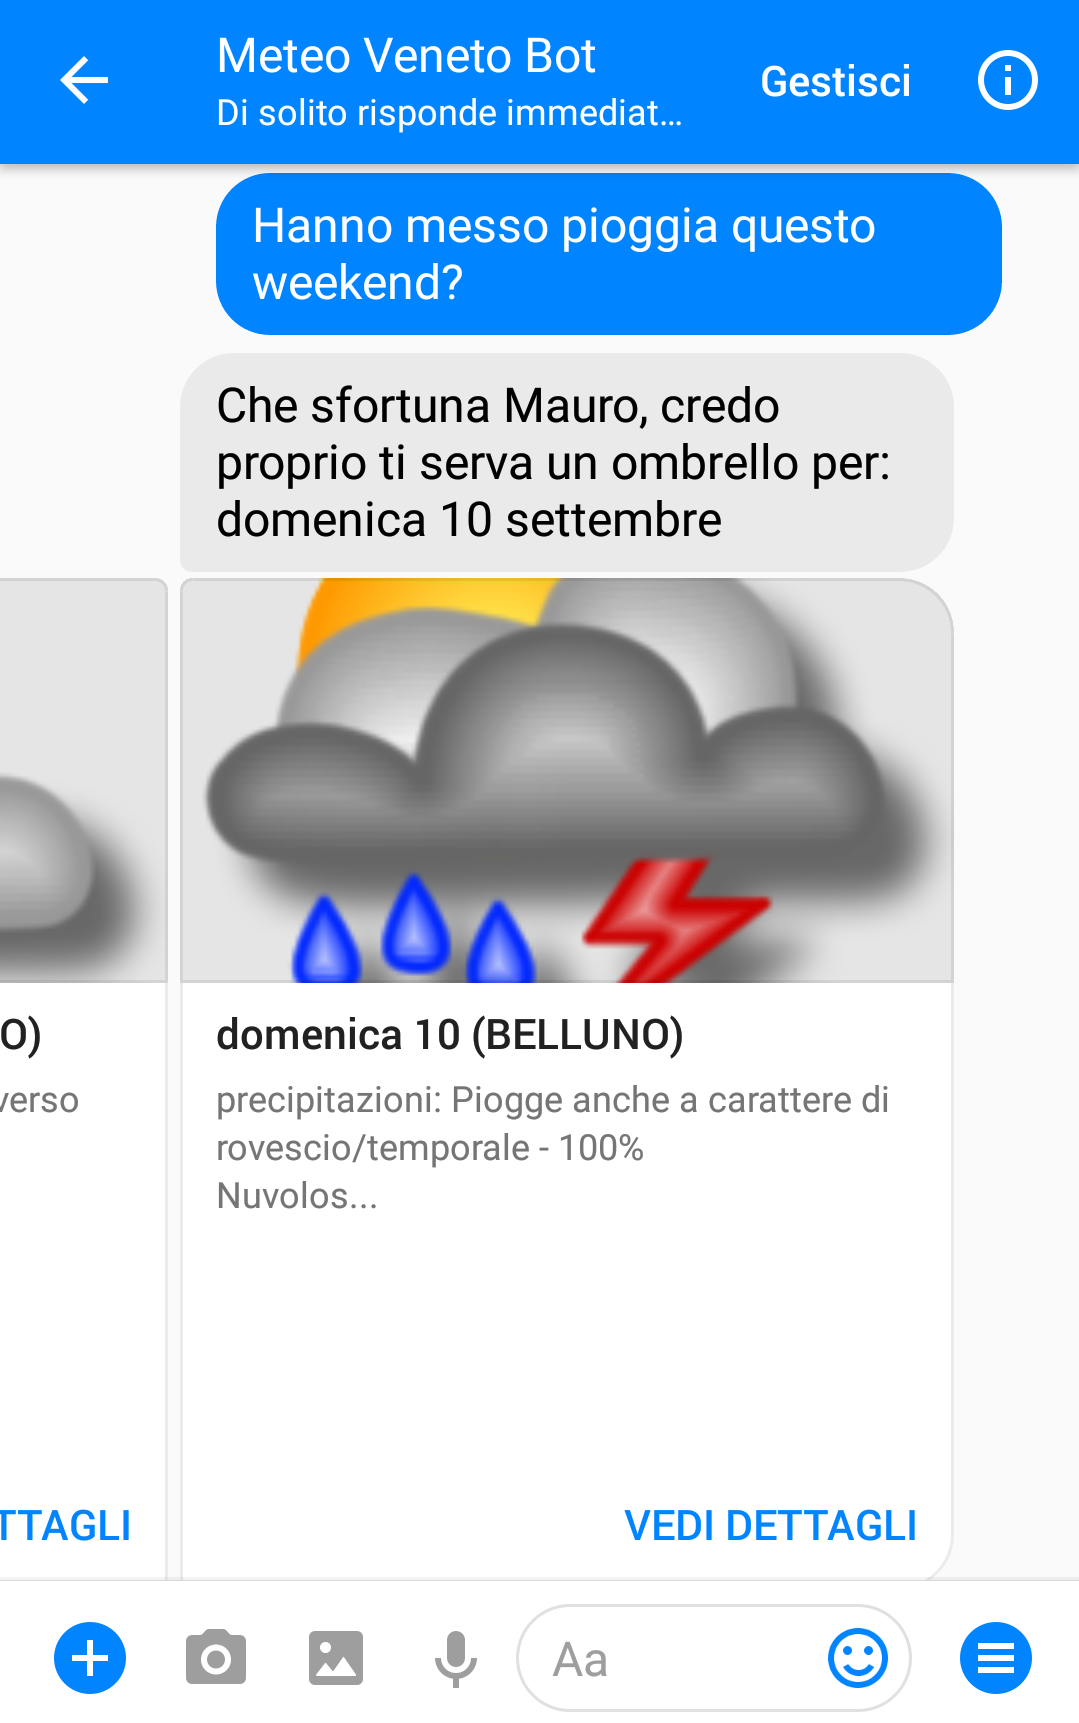
\includegraphics[scale=0.12]{../Immagini/richiesta_pioggia2.png}
		\caption{Didascalia comune alle due figure}
	\end{figure}
	\item \textbf{richiesta\_nebbia}: permette all'utente di chiedere se è prevista nebbia in una specifica giornata o un periodo di tempo (es. weekend), in un determinato comune. La risposta è formata da due messaggi: il primo mostra le giornate dove è prevista nebbia, tra quelle richieste dall'utente, il secondo contiene i caroselli delle previsioni.
	\begin{figure}[!h]
		\centering
		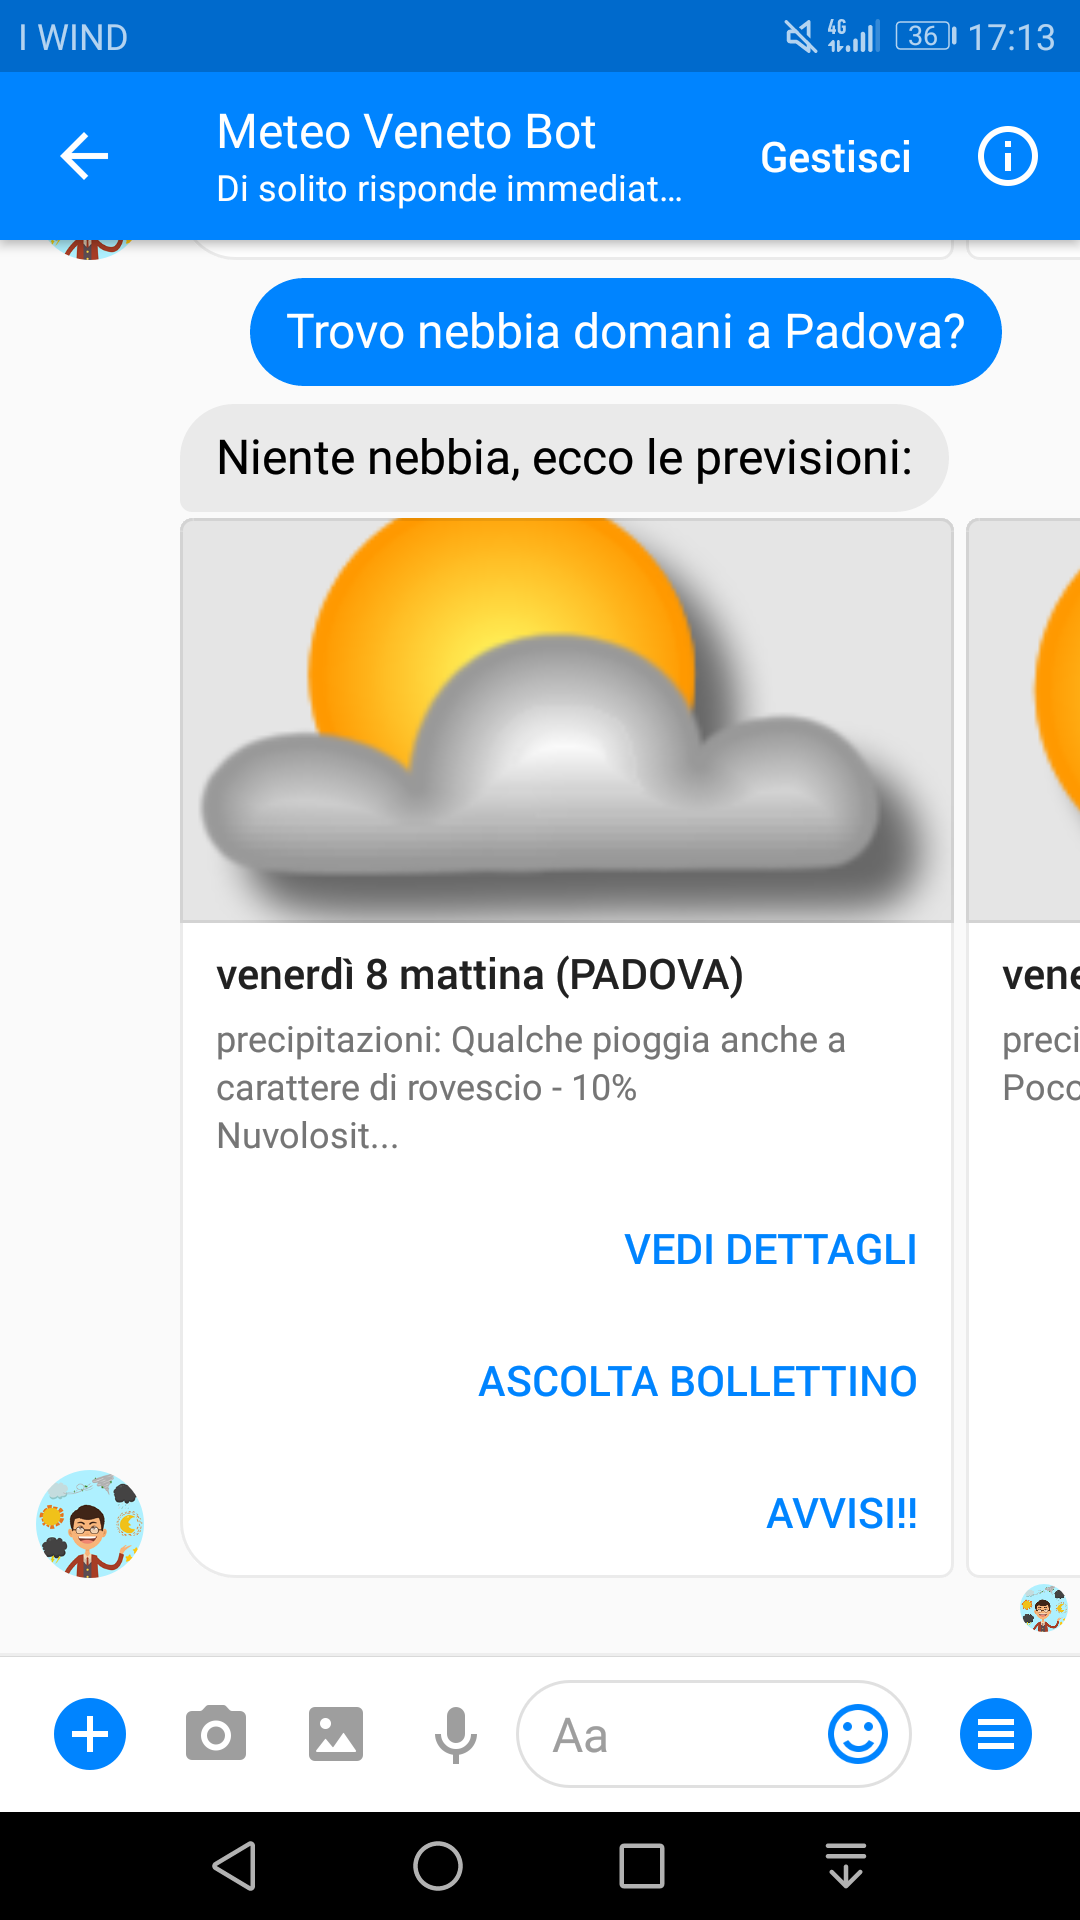
\includegraphics[scale=0.12]{../Immagini/richiesta_nebbia.png}
		\caption{Esempio di }
	\end{figure}
	\item \textbf{richiesta\_neve}: permette all'utente di chiedere se è prevista neve in una specifica giornata o un periodo di tempo (es. weekend), in un determinato comune. La risposta è formata da due messaggi: il primo mostra le giornate dove è prevista neve, tra quelle richieste dall'utente, il secondo contiene i caroselli delle previsioni.
	\begin{figure}[!h]
		\centering
		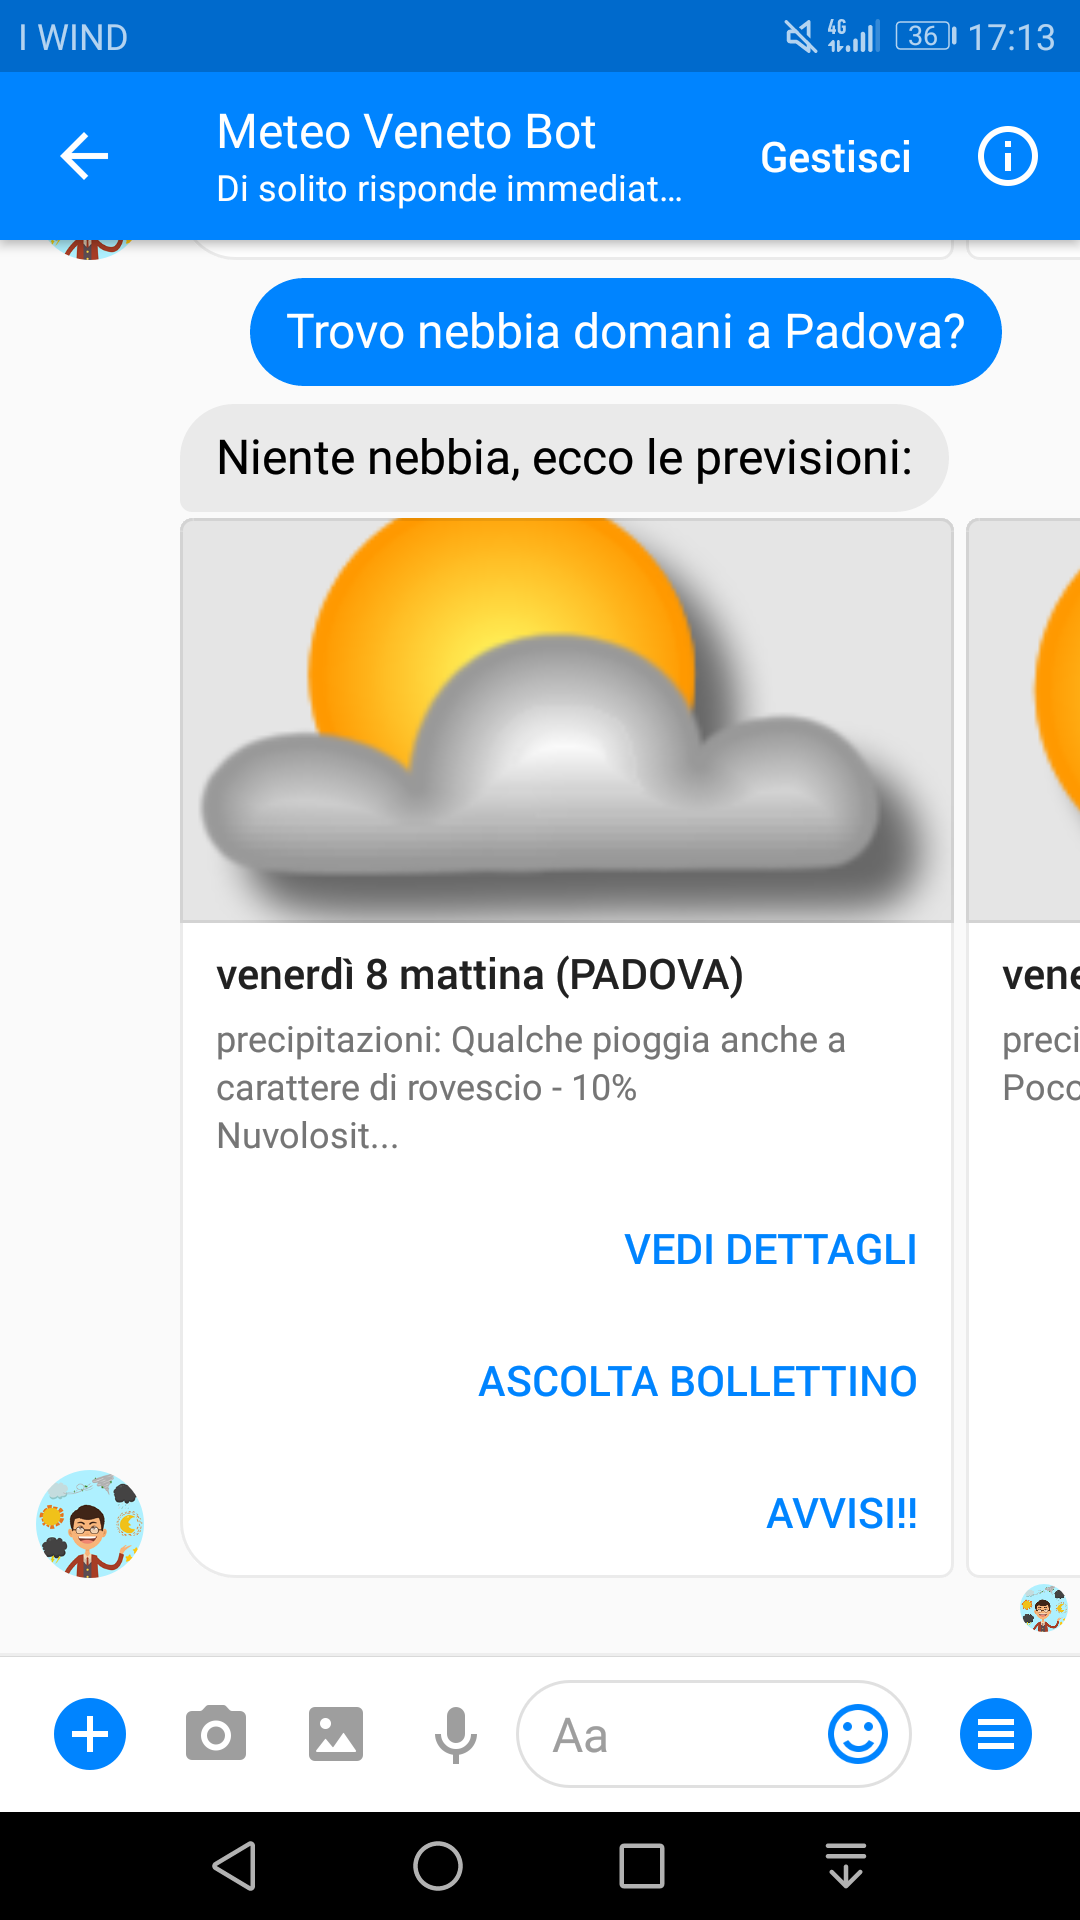
\includegraphics[scale=0.12]{../Immagini/richiesta_nebbia.png}
		\caption{Esempio di }
	\end{figure}
	\item \textbf{richiesta\_bel\_tempo}: permette all'utente di chiedere se è previsto bel tempo in una specifica giornata o un periodo di tempo (es. weekend), in un determinato comune. La risposta è formata da due messaggi: il primo mostra le giornate dove è previsto bel tempo, tra quelle richieste dall'utente, il secondo contiene i caroselli delle previsioni.
	\begin{figure}[!h]
		\centering
		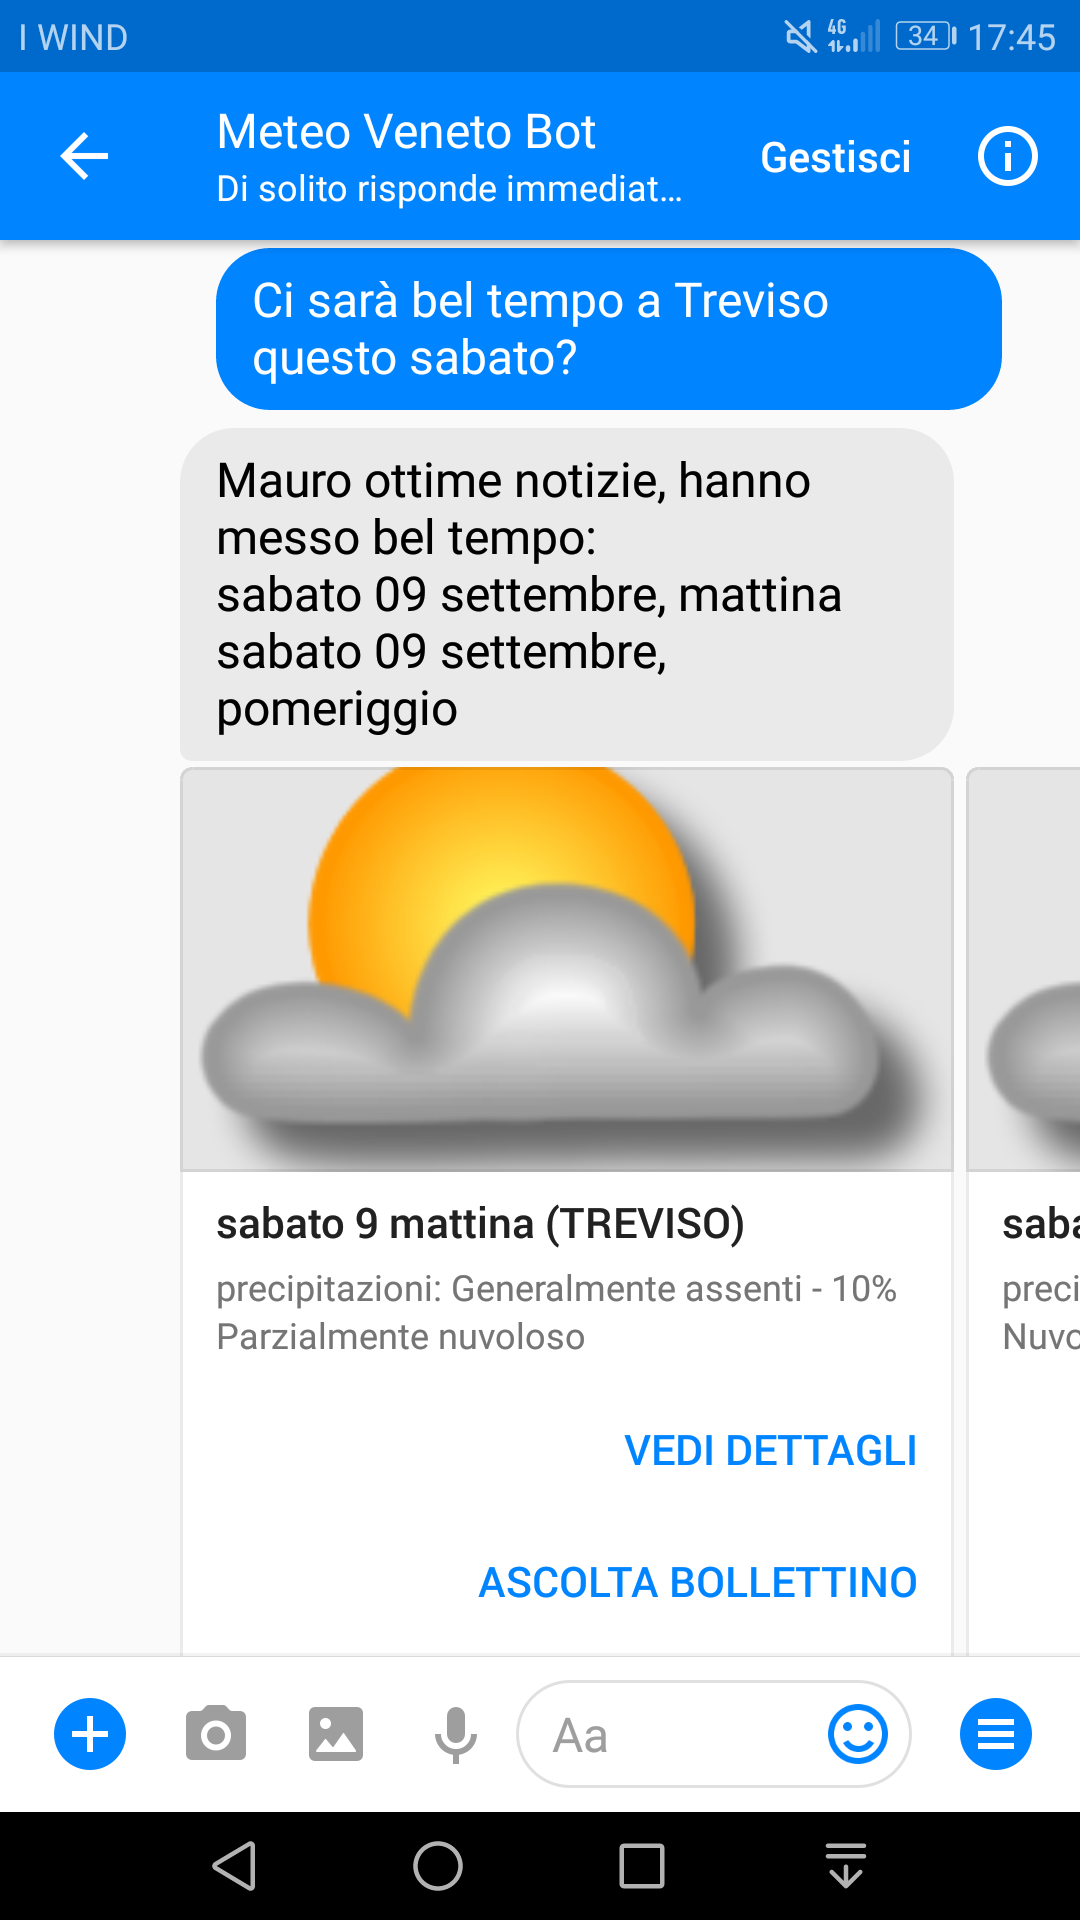
\includegraphics[scale=0.12]{../Immagini/richiesta_bel_tempo.png}
		\caption{Esempio di }
	\end{figure}
	\item \textbf{richiesta\_brutto\_tempo}: permette all'utente di chiedere se è previsto brutto tempo in una specifica giornata o un periodo di tempo (es. weekend), in un determinato comune. La risposta è formata da due messaggi: il primo mostra le giornate dove è previsto brutto tempo, tra quelle richieste dall'utente, il secondo contiene i caroselli delle previsioni.
	\begin{figure}[!h]
		\centering
		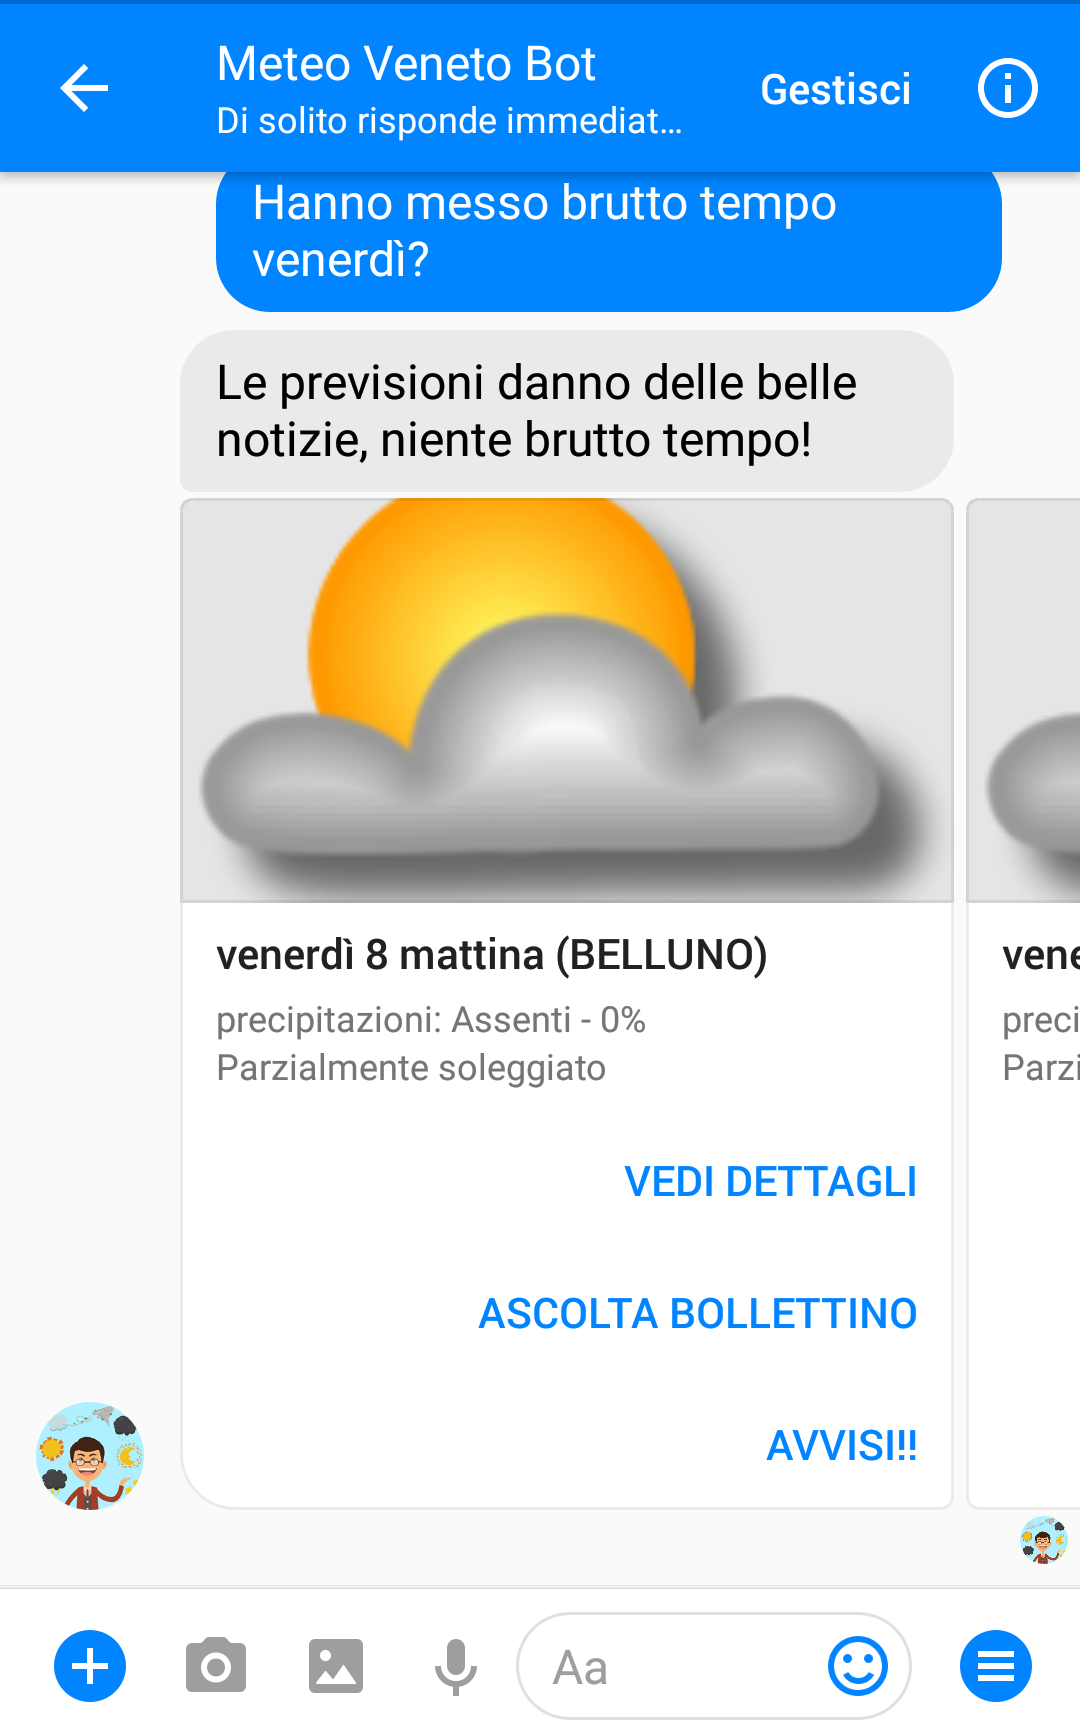
\includegraphics[scale=0.12]{../Immagini/richiesta_brutto_tempo.png}
		\caption{Esempio di }
	\end{figure}
	\item \textbf{richiesta\_temperature}: permette all'utente di chiedere le temperature previste in una specifica giornata o un periodo di tempo (es. weekend), in un determinato comune. La risposta contiene le temperature massimi e minime previste fornite da ARPA Veneto.
	\begin{figure}[!h]
		\centering
		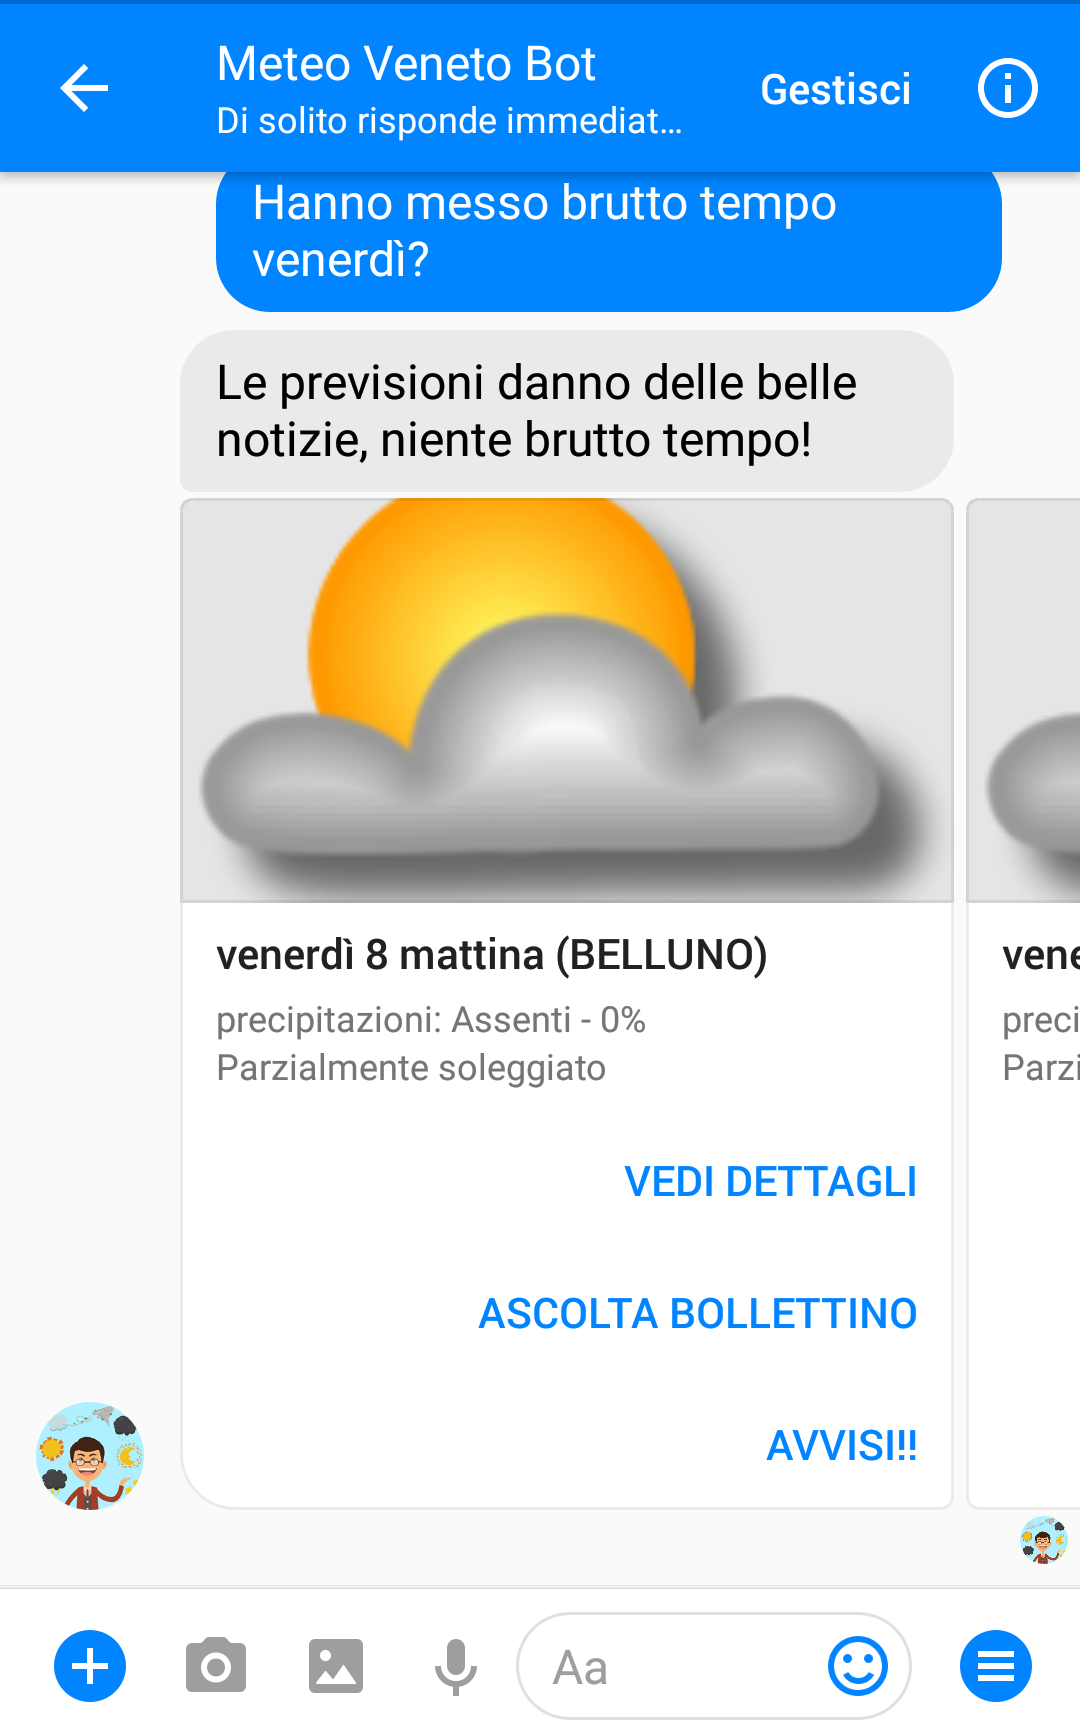
\includegraphics[scale=0.12]{../Immagini/richiesta_brutto_tempo.png}
		\caption{Esempio di }
	\end{figure}
	\item \textbf{ascolta\_bollettino}: permette all'utente di chiedere il bollettino audio emesso da ARPA Veneto ogni giorno. La risposta contiene il file audio richiesto.
	\begin{figure}[!h]
		\centering
		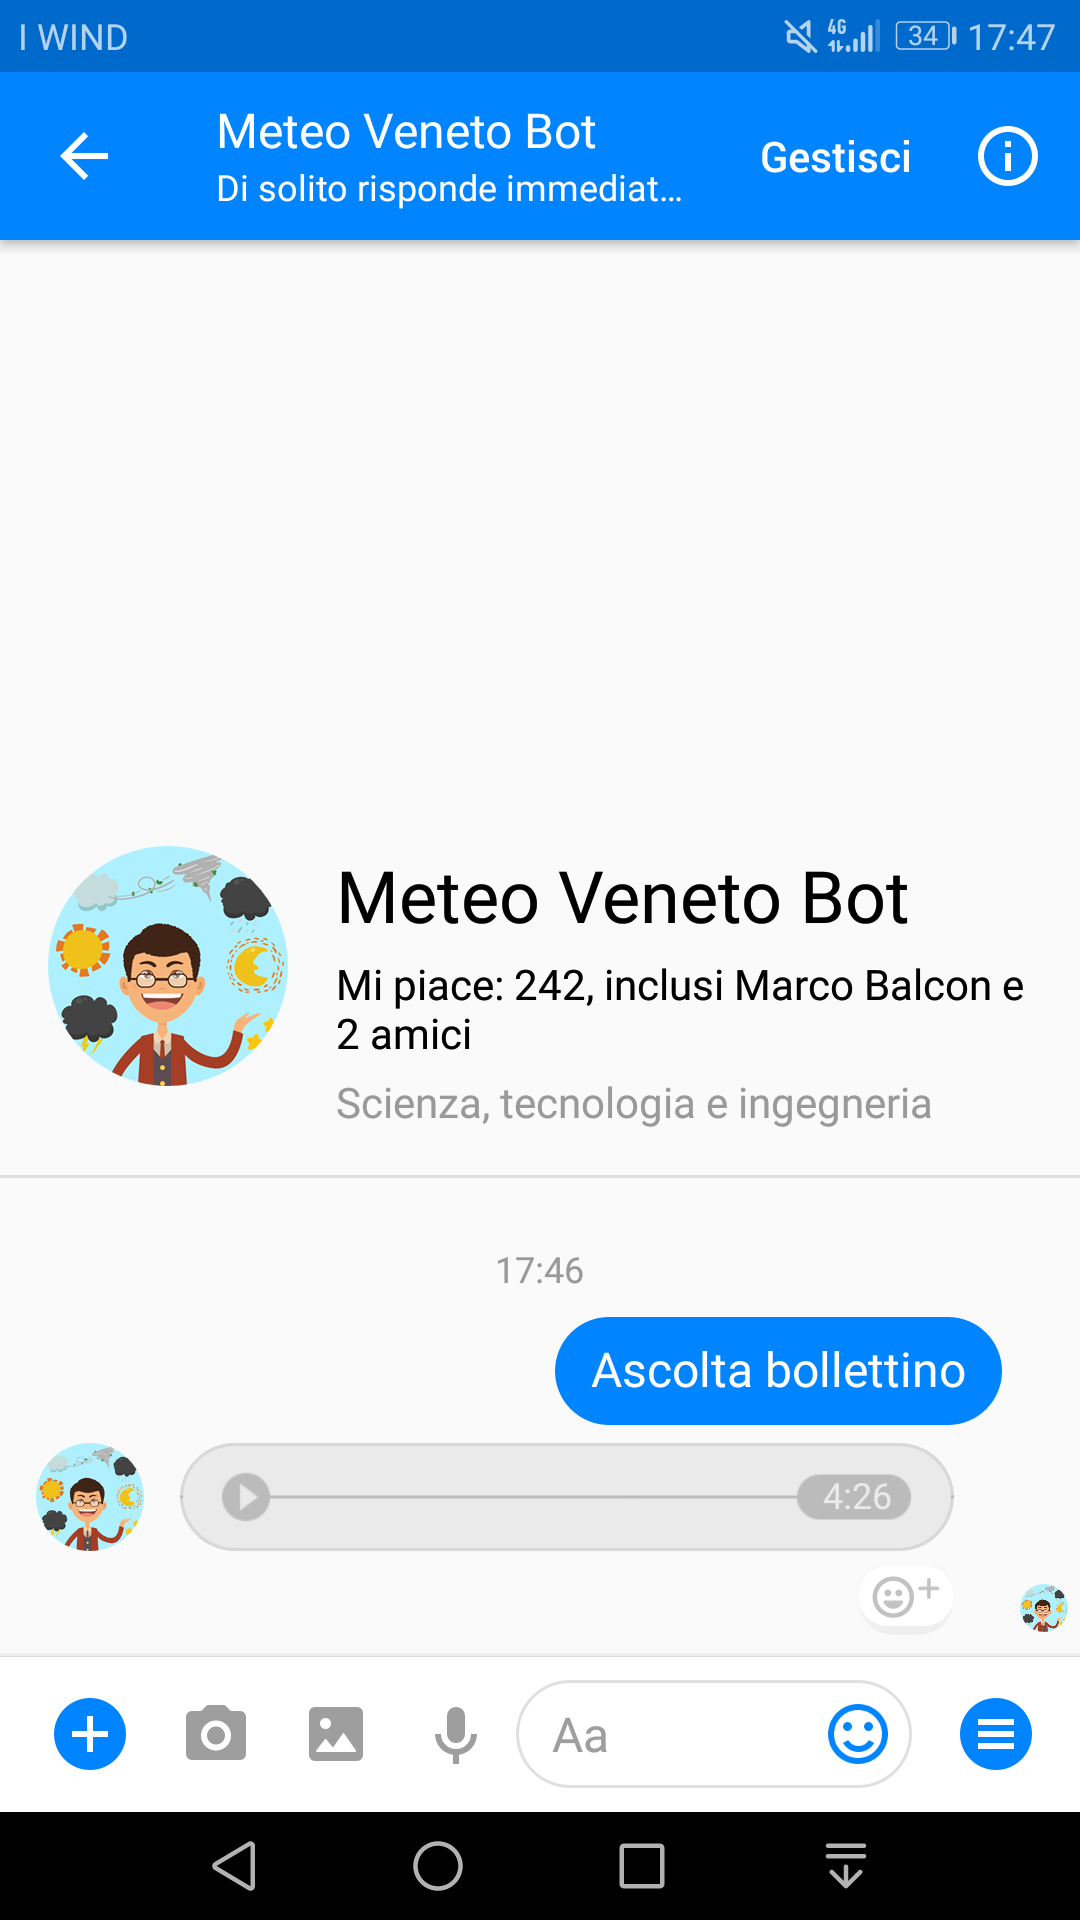
\includegraphics[scale=0.12]{../Immagini/bollettino.png}
		\caption{Esempio di }
	\end{figure}
	\item \textbf{fenomeni\_particolari}: permette all'utente di chiedere se sono presenti avvisi o fenomeni particolari emessi da ARPAV. La risposta contiene questi avvisi, se presenti.
	\begin{figure}[!h]
		\centering
		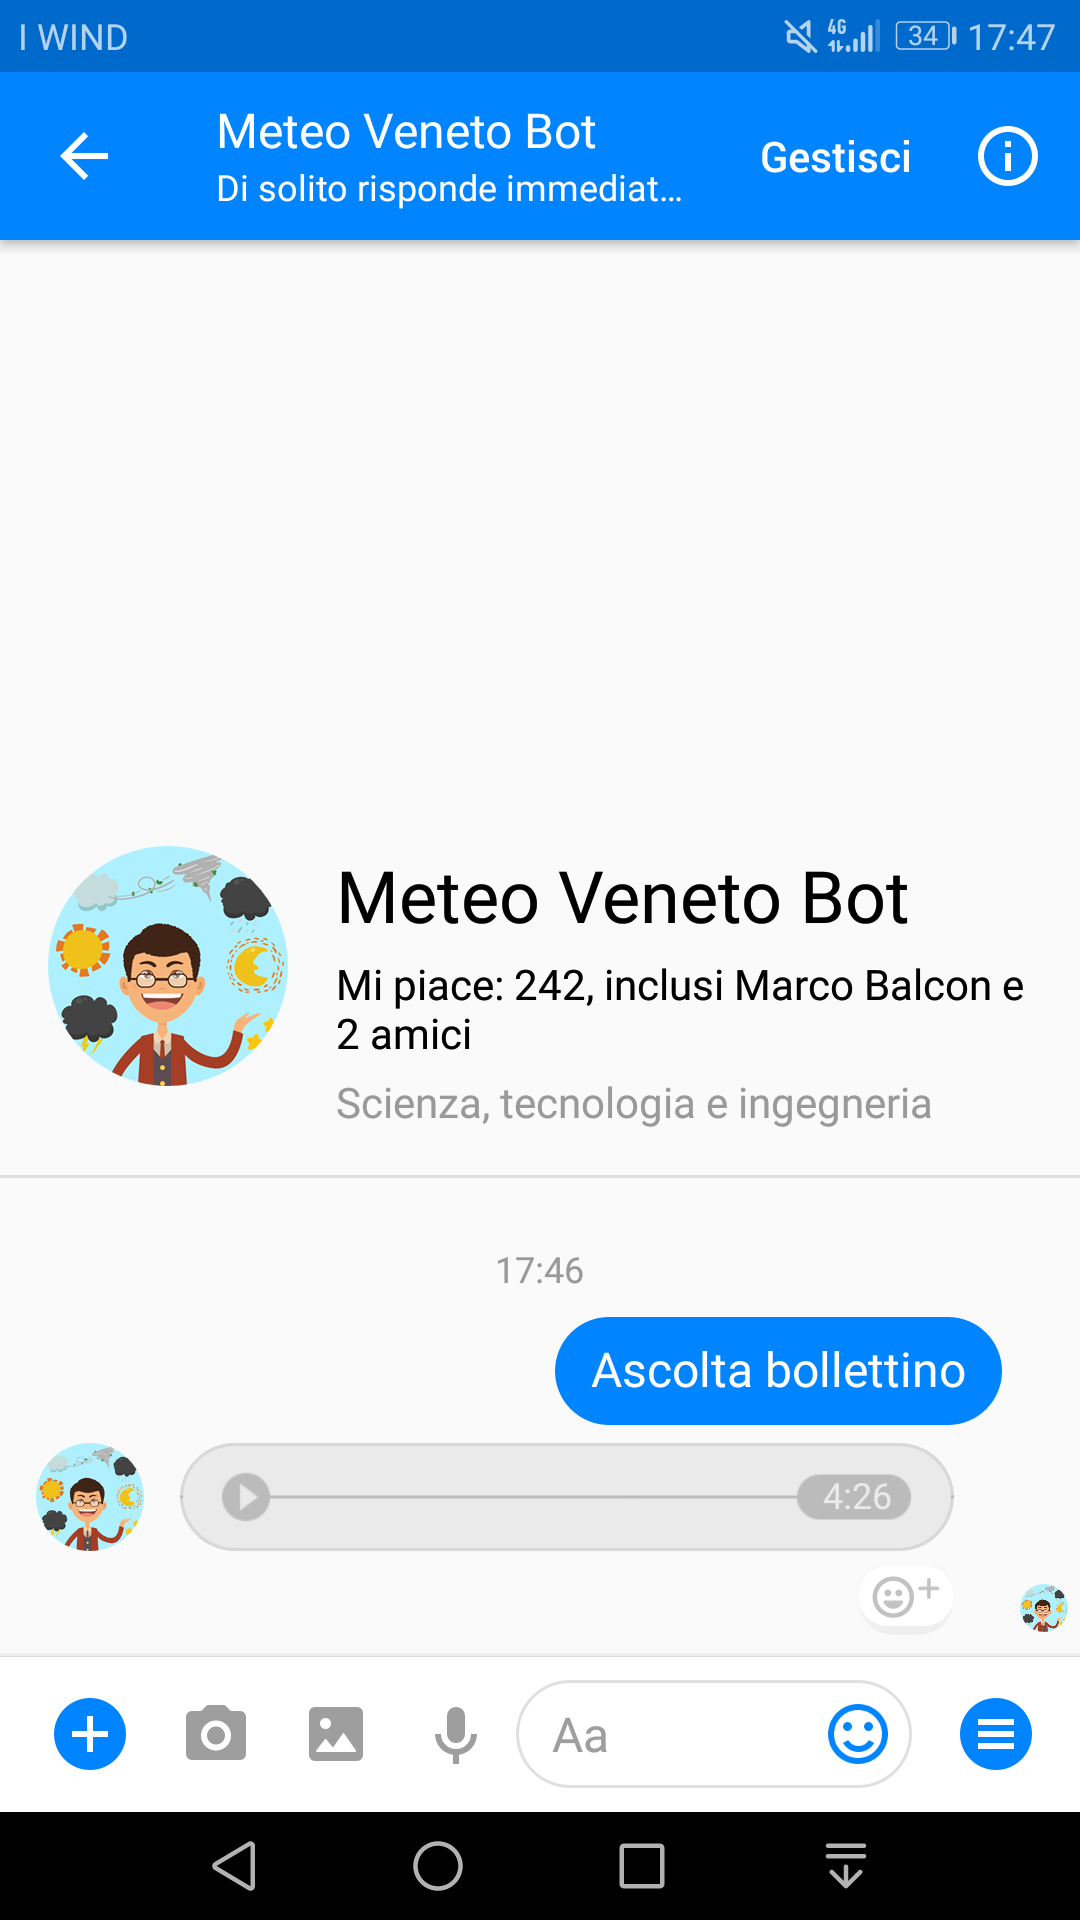
\includegraphics[scale=0.12]{../Immagini/bollettino.png}
		\caption{Esempio di }
	\end{figure}

\end{itemize}
\newpage
\subsubsection{Entity}
Nella progettazione di questo \emph{agent} ho creato queste nuove \emph{entities}:
\begin{itemize}
	\item \textbf{fenomeni atmosferici}: ho creato quattro \emph{entities} per \textbf{sole}, \textbf{pioggia}, \textbf{neve}, \textbf{nebbia}, in modo da gestire i possibili sinonimi che un utente può scrivere;
	\item \textbf{time}: si tratta di una \emph{composite entity} per gestire gli orari e le date scritte dall'utente. In particolare questa \emph{entity} combina tre \emph{system entity} fornite da api.ai:
	\begin{itemize}
		\item \textbf{@sys.date}: per le date in formato standard (es. 31 agosto);
		\item \textbf{@sys.date-period}: per un periodo di tempo formato da più giorni (es. weekend);
		\item \textbf{@sys.time-period}: per una parte del giorno (es. mattina, pomeriggio, notte);
	\end{itemize}
Combinando queste \emph{entities} l'utente può specificare precisamente le previsioni che desidera ricevere. Può infatti porre al \gls{chatbot} domande del tipo: \emph{"Che tempo farà domani sera?"}, \emph{"Dimmi le previsioni per il prossimo weekend"}, \emph{"Ci sarà il sole venerdì pomeriggio?"}.
\end{itemize}
\begin{figure}[!h]
	\centering
	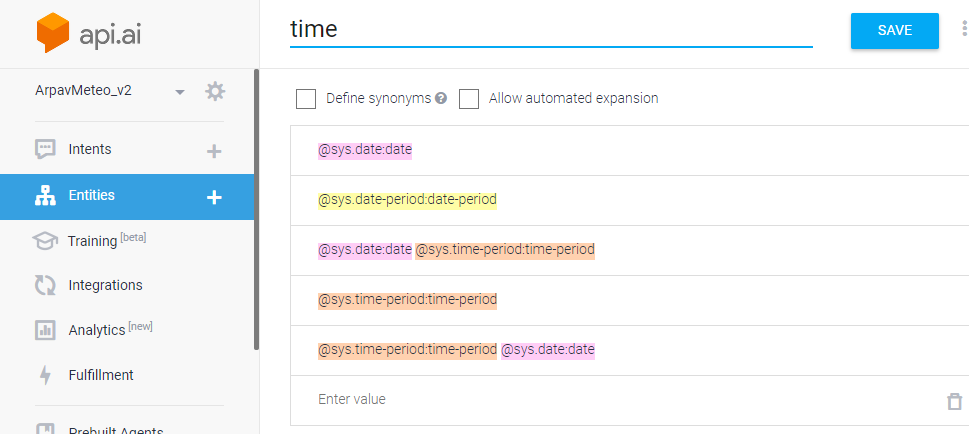
\includegraphics[scale=0.5]{../Immagini/time.png}
	\caption{Entity time definita nell'agent}
\end{figure}
\newpage
\section{Progettazione delle componenti}
Per quanto riguarda la progettazione delle componenti da aggiungere al software aziendale ho deciso di creare due classi per ciascun \gls{chatbot}, con un comportamento simile. La prima ha il compito di:
\begin{itemize}
	\item \textbf{interrogare api.ai}, costruendo il messaggio da inviare con il token dell'agent, l'input e il sessionId dell'utente;
	\item \textbf{analizzare la risposta}, invocando il metodo corretto a seconda del valore del campo \emph{action} del \gls{JSON}.
\end{itemize}
La seconda classe invece contiene tutti i metodi che rappresentano la logica del \gls{chatbot}, analizzando i \emph{parameters} del \gls{JSON} ritornato da api.ai e formulando la risposta da visualizzare nella chat. Questi metodi hanno riutilizzato dei componenti già presenti nel software, per costruire modelli di risposta già previsti nel \gls{chatbot} prima del mio arrivo.


\section{Jaro Winkler distance}
Durante l'attività di progettazione mi sono reso conto come fosse necessario gestire un possibile errore di scrittura dell'utente in una delle sue domande, soprattutto nelle parole fondamentali per formulare le risposte, come ad esempio il nome di un comune per il \gls{chatbot} del meteo o il nome di una conferenza in quello degli eventi. In un primo momento infatti l'input dell'utente veniva utilizzato direttamente nelle \emph{query} \gls{SQL} per interrogare il database ed ottenere i dati di interesse, soprattutto attraverso l'operatore \emph{"LIKE"}. In questo modo però non è possibile gestire il caso in cui un utente scriva ad esempio il comune "Padvoa", intendendo Padova. \\
Per ovviare a questo problema quindi è stato deciso di introdurre, dopo uno studio delle possibili soluzioni, la Jaro Winkler distance\footcite{jaro}, ossia una metrica che misura la "distanza" tra due stringhe per capire quanto esse siano simili tra loro. Grazie a questa accortezza, nel caso di errore di scrittura, il \gls{chatbot} è in grado di:
\begin{itemize}
	\item fornire una serie di opzioni di cosa secondo lui l'utente voleva scrivere, dando la possibilità ad esso di selezionare quella giusta;
	\item fornire i dati richiesti dall'utente nel caso ci sia un'unica corrispondenza simile a quanto scritto dall'utente nel database.
\end{itemize}
\begin{figure}[!h]
	\centering
	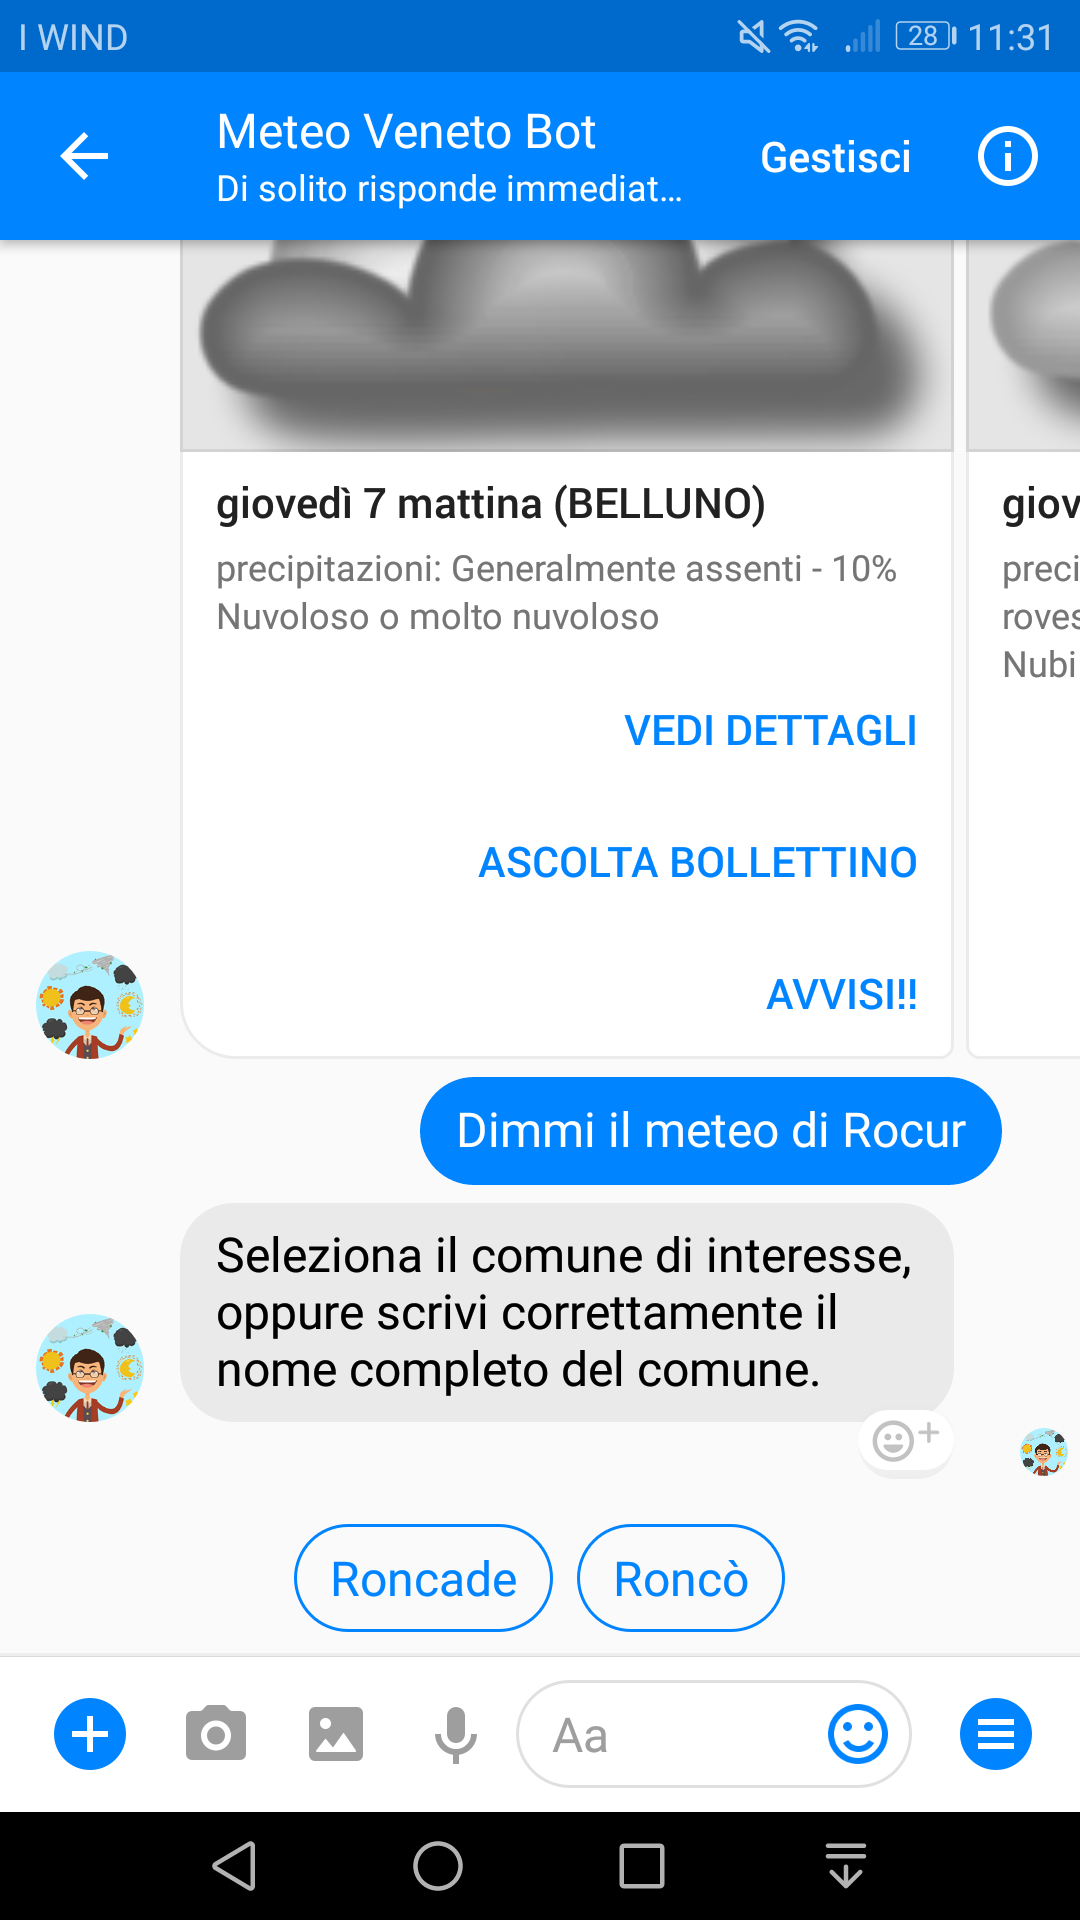
\includegraphics[scale=0.12]{../Immagini/meteo_scelta.png}
	\caption{Esempio di utilizzo della Jaro Winkler distance}
\end{figure}
        	    % Progettazione
% !TEX encoding = UTF-8
% !TEX TS-program = pdflatex
% !TEX root = ../tesi.tex

%**************************************************************
\chapter{Verifica e validazione}
\label{cap:verifica}

Durante il mio stage lo sviluppo delle nuove funzionalità ha portato alla minimizzazione dei tempi di verifica e validazione. Tale decisione è stata presa in comune accordo con il tutor aziendale, in quanto lo scopo dello stage mirava all’estensione di più funzionalità possibili, che potranno essere testate successivamente dall’azienda.
Questa decisione è inoltre appoggiata dalla metodologia \emph{agile} utilizzata nello sviluppo del progetto, la quale definisce la qualità del software come la capacità di soddisfare i bisogni del cliente piuttosto che soddisfare metriche fissata a priori.
In ogni caso, vista l'importanza di queste attività, sono state adottate tecniche di analisi statica e analisi dinamica per il codice sorgente, al fine di verificarne e validarne il comportamento.

\section{Analisi statica}
L’analisi statica è il processo di valutazione di un sistema o di un suo componente basato sulla sua forma, struttura, contenuto, documentazione senza che esso sia eseguito. Gli strumenti di analisi statica del codice consentono di individuare porzioni di codice del proprio programma ad alta probabilità di errore. Avendo a disposizione una lista di linee di codice sospette, un programmatore può poi verificare se siano presenti errori e, in caso positivo, rivedere il codice corrispondente e correggere le problematiche individuate. \\
In particolare sono state utilizzate queste tecniche di analisi statica:
\begin{itemize}
	\item \textbf{\emph{code inspections}} o \textbf{\emph{reviews}}, in cui si effettua una lettura ed analisi di gruppo
con l’ausilio della documentazione. Qui si analizza il codice secondo delle \emph{checklist}, ossia liste contenenti dei tipici errori di programmazione, indipendenti dal linguaggio usato e dal codice in esame;	
	\item \emph{walktrough\textbf{•}}, un’analisi dinamica con casi di test svolti a mano.
\end{itemize}

\section{Analisi dinamica}
L’analisi dinamica è il processo di valutazione di un sistema software o di un suo componente basato sulla osservazione del suo comportamento in esecuzione. Una volta soddisfatti tutti gli obiettivi definiti con l’azienda, l’attività di validazione è stata svolta tramite analisi dinamica grazie alla progettazione di alcuni test. I test sviluppati sono di due tipi:
\begin{itemize}
	\item \textbf{ciao}
\end{itemize}

\section{Verifica e validazione api.ai}
Gran parte del progetto di stage verteva nell'istruire gli \emph{agent} di api.ai per gestire le domande degli utenti fatte attraverso i \gls{chatbot}. Essendo quindi una parte molto importante del prodotto sono stati creati alcuni test per verificare e validare le sue funzionalità. 				% Testing e realizzione
% !TEX encoding = UTF-8
% !TEX TS-program = pdflatex
% !TEX root = ../tesi.tex

%**************************************************************
\chapter{Conclusioni}
\label{cap:conclusioni}

\section{Raggiungimento degli obiettivi}
Come descritto nella sezione \ref{obiettivi}, io e il mio tutor aziendale abbiamo stilato una serie di obiettivi da raggiungere nelle 300 ore di stage, divisi in obiettivi obbligatori e desiderabili. \\ 
Gli obiettivi obbligatori si concentravano sull'analisi di mercato dei principali strumenti per il \gls{NLP} e sullo sviluppo delle funzionalità del prodotto, integrandole nell'architettura già creata dall'azienda. Gli obiettivi desiderabili si focalizzavano invece nel testare in modo approfondito il risultato ottenuto, attraverso l'utilizzo dei \glspl{Chatbot} di Facebook Messenger in un ambiente locale. 
Al termine dello stage tutti gli obiettivi prefissati sono stati soddisfatti nei tempi previsti. Questo è stato possibile grazie alla buona pianificazione delle tempistiche necessarie allo svolgimento dei vari compiti, sia da parte dello stagista che da parte dell'azienda. La metodologia di sviluppo \emph{Agile} si è inoltre dimostrata molto efficace, permettendomi di rispondere in modo rapido ai cambiamenti proposti dall'azienda durante il mio lavoro. 
\section{Conoscenze acquisite}
Da un punto di vista formativo l'attività di stage è stata sicuramente molto positiva. Queste 300 ore mi hanno permesso di mettermi alla prova, dandomi un riscontro su quanto gli anni universitari mi hanno preparato, sia nell'ambito delle mie conoscenze, sia da quello umano, per affrontare il mondo del lavoro.


Lo stage ha sicuramente arricchito il mio bagaglio personale di competenze tecniche, dandomi una panoramica delle procedure e delle attività che giornalmente si svolgono all'interno di un'azienda. Questo mi ha inoltre permesso di rendermi conto quanto una buona collaborazione tra i membri di un team sia fondamentale nello sviluppo di un prodotto, di qualsiasi tipo si tratti.
Le competenze acquisite non riguardano solamente il campo informatico, grazie alle nuove tecnologie utilizzate, ma anche le mie capacità organizzative, fondamentali per il rispetto dei vincoli e delle scadenze imposte dall'azienda. Ho dovuto infatti pianificare in modo preciso il lavoro delle mie settimane, per garantire ad \azienda{} la portata a termine del mio progetto, senza dover impiegare un dipendente per adempire alle mie mancanze. 

\section{Valutazione retrospettiva}
Al termine del mio periodo di stage ho potuto fare delle valutazioni sul lavoro da me svolto. Per quanto riguarda il progetto a me assegnato sono rimasto soddisfatto per averlo realizzato nei tempi prestabiliti, rispettando scadenze e vincoli aziendali. Mi sarebbe piaciuto avere un'ulteriore settimana per verificare quanto il mio prodotto fosse pronto per la distribuzione al pubblico. Questo sarebbe stato molto importante anche per valutare e gestire le effettive domande che una persona comune scrive ad un \gls{Chatbot}, in modo da migliorare la percentuale di richieste soddisfatte dallo stesso. Purtroppo come già detto il numero limitato di ore non mi ha permesso di svolgere questo ulteriore passo nello sviluppo del mio prodotto, anche se con le indicazione che ho fornito all'azienda gli sviluppatori saranno in grado di farlo al mio posto.\\ \\
Il prodotto ottenuto può anche essere migliorato da \azienda{} introducendo nuove funzionalità per il cliente, anche in base ai feedback degli stessi. Ad esempio nel \gls{Chatbot} del meteo si potrebbe introdurre la possibilità di valutare la posizione dell'utente ad ogni domanda per fornire delle risposte più precise. L'azienda inoltre stava pensando alla creazione di altri \gls{Chatbot} molto simili per la piattaforma di Telegram, per incrementare il numero di utenti e rivolgersi principalmente ai giovani. In ogni caso questi strumenti hanno molti possibili miglioramenti considerando che sono tecnologie relativamente nuove.

\section{Valutazione personale}
Nel complesso ritengo la mia esperienza di stage molto positiva ed istruttiva. L'inserimento, se pur breve, in un contesto aziendale permette di far capire ad uno studente quanto siano differenti il mondo del lavoro e quello universitario, in modo da cogliere gli aspetti fondamentali che solamente esperienze di questo tipo ti possono dare.

Per quanto riguarda l'azienda che mi ha ospitato si è rivelata molto disponibile ed accogliente, mi ha guidato nei miei primi giorni di stage chiarendomi tutti i dubbi o le mie mancanze dal punto di vista tecnico. Il progetto che mi è stato proposto mi ha permesso di confrontarmi con nuove tecnologie, mettendo alla prova la mia capacità di apprendere nuovi concetti in breve tempo. Mi sono inoltre reso conto di quanto le mie esperienze universitarie, soprattutto per quanto riguarda i progetti individuali e di gruppo svolti, si sono dimostrate fondamentali per organizzare e gestire una quantità di lavoro che mai avevo dovuto affrontare.

Mi ritengo quindi molto soddisfatto dell'esperienza fatta, in un campo come l'informatica dove apprendere nuove nozioni e competenze resta un aspetto fondamentale per crescere e migliorare.     			% Conclusioni
%**************************************************************
% Materiale finale
%**************************************************************
\backmatter

\printglossaries

\end{document}